% !TeX root = stable-vnmm2d.tex
%% 
%% Copyright 2007-2025 Elsevier Ltd
%% 
%% This file is part of the 'Elsarticle Bundle'.
%% ---------------------------------------------
%% 
%% It may be distributed under the conditions of the LaTeX Project Public
%% License, either version 1.3 of this license or (at your option) any
%% later version.  The latest version of this license is in
%%    http://www.latex-project.org/lppl.txt
%% and version 1.3 or later is part of all distributions of LaTeX
%% version 1999/12/01 or later.
%% 
%% The list of all files belonging to the 'Elsarticle Bundle' is
%% given in the file `manifest.txt'.
%% 
%% Template article for Elsevier's document class `elsarticle'
%% with numbered style bibliographic references
%% SP 2008/03/01
%% $Id: elsarticle-template-num.tex 272 2025-01-09 17:36:26Z rishi $
%%
\documentclass[preprint,12pt]{elsarticle}

%% Use the option review to obtain double line spacing
%% \documentclass[authoryear,preprint,review,12pt]{elsarticle}

%% Use the options 1p,twocolumn; 3p; 3p,twocolumn; 5p; or 5p,twocolumn
%% for a journal layout:
%% \documentclass[final,1p,times]{elsarticle}
%% \documentclass[final,1p,times,twocolumn]{elsarticle}
%% \documentclass[final,3p,times]{elsarticle}
%% \documentclass[final,3p,times,twocolumn]{elsarticle}
%% \documentclass[final,5p,times]{elsarticle}
%% \documentclass[final,5p,times,twocolumn]{elsarticle}

%% For including figures, graphicx.sty has been loaded in
%% elsarticle.cls. If you prefer to use the old commands
%% please give \usepackage{epsfig}

%% The amssymb package provides various useful mathematical symbols
\usepackage{amssymb}
%% The amsmath package provides various useful equation environments.
\usepackage{amsmath}
%% The amsthm package provides extended theorem environments
%% \usepackage{amsthm}
\usepackage{amsfonts}
%% The lineno packages adds line numbers. Start line numbering with
%% \begin{linenumbers}, end it with \end{linenumbers}. Or switch it on
%% for the whole article with \linenumbers.
%% \usepackage{lineno}
% --- Pacotes e Definição do Ambiente de Teoremas ---
\usepackage{amsthm}
\newtheorem{theorem}{Theorem}
\newtheorem{proposition}{Proposition}
\usepackage{graphicx}                 % Para inclusão de figuras
\usepackage{tabularx}
\usepackage{booktabs}                 % Para tabelas elegantes no padrão IEEE/Elsevier
\usepackage{bm}                       % Para notação de vetores em negrito
\usepackage{microtype}                % Melhora o espaçamento de palavras
\usepackage{float}                    % Controle preciso de posicionamento de figuras e tabelas [H], [!htbp]
\usepackage[pdfpagelabels=false]{hyperref} % Cria links ativos para equações e referências
\hypersetup{
    colorlinks=true,
    linkcolor=blue,
    citecolor=blue,
    urlcolor=blue,
    pdfencoding=auto,
    hypertexnames=false
}
\pdfstringdefDisableCommands{%
  \def\corref#1{}%
  \def\cnotenum#1{}%
}
\setlength{\emergencystretch}{2em}
\hbadness=3000

\journal{Engineering Analysis with Boundary Elements}

\begin{document}

\begin{frontmatter}

%% Title, authors and addresses

%% use the tnoteref command within \title for footnotes;
%% use the tnotetext command for theassociated footnote;
%% use the fnref command within \author or \affiliation for footnotes;
%% use the fntext command for theassociated footnote;
%% use the corref command within \author for corresponding author footnotes;
%% use the cortext command for theassociated footnote;
%% use the ead command for the email address,
%% and the form \ead[url] for the home page:
%% \title{Title\tnoteref{label1}}
%% \tnotetext[label1]{}
%% \author{Name\corref{cor1}\fnref{label2}}
%% \ead{email address}
%% \ead[url]{home page}
%% \fntext[label2]{}
%% \cortext[cor1]{}
%% \affiliation{organization={},
%%             addressline={},
%%             city={},
%%             postcode={},
%%             state={},
%%             country={}}
%% \fntext[label3]{}

% --- TÍTULO DO ARTIGO ---
\title{A Stabilized 2D Vector Nodal Meshless Method on Irregular Point Clouds: Complete Polynomial Basis and Automated Support Selection}


%% use optional labels to link authors explicitly to addresses:
%% \author[label1,label2]{}
%% \affiliation[label1]{organization={},
%%             addressline={},
%%             city={},
%%             postcode={},
%%             state={},
%%             country={}}
%%
%% \affiliation[label2]{organization={},
%%             addressline={},
%%             city={},
%%             postcode={},
%%             state={},
%%             country={}}

\author[ufmg]{Renato C. Mesquita\corref{cor1}}
\ead{renato@ufmg.br}
\author[ufmg]{Elson J. da Silva}
\author[ufmg]{Bárbara M. F. Gonçalves}
\author[ufmg]{Luilly A. G. Ortiz}

\affiliation[ufmg]{organization={Department of Electrical Engineering, Universidade Federal de Minas Gerais},
             addressline={Av. Antônio Carlos, 6627}, 
             city={Belo Horizonte},
             postcode={31270-901}, 
             state={MG},
             country={Brazil}}

\cortext[cor1]{Corresponding author}

%% Abstract
\begin{abstract}
The Vector Nodal Meshless Method (VNMM) provides an attractive alternative to the Edge Finite Element Method (EFEM) by defining local $H(\mathrm{curl})$-regular vector approximations through point-collocated nodes assigned unit vector directors. However, standard formulations based on N\'ed\'elec's incomplete solenoidal polynomial space ($\mathcal{L}^1$) exhibit a notable limitation when applied to unstructured point distributions: the numerical approximation of the curl operator $(\nabla \times \vec{E})$ tends to stagnate at an $\mathcal{O}(1)$ relative error plateau.

In this paper, we address this fundamental issue by presenting two primary methodological contributions to the 2D VNMM:
First, we adopt the complete linear polynomial vector space $\mathcal{P}^1 = \mathcal{P}_1 \times \mathcal{P}_1$ ($6$ support nodes per evaluation point), which resolves all four components of the local Jacobian tensor, removing the derivative aliasing mechanism identified for the incomplete $\mathcal{L}^1$ basis and overcoming the $\mathcal{O}(1)$ curl error stagnation plateau.
Second, to ensure algebraic stability on irregular node distributions, we develop an automated support selection algorithm combining $k$-d tree spatial queries with scale-dependent placement matrix determinant thresholding and an absolute tolerance floor, filtering ill-conditioned stencils without requiring background mesh connectivity.

To appraise these contributions, we conduct a systematic evaluation divided into numerical verification and spectral validation stages.
In the numerical verification stage, we first verify the exact algebraic and topological local dual equivalence between the $\mathcal{L}^1$ VNMM and canonical Whitney 1-form edge elements on simplicial meshes down to machine precision ($\approx 10^{-16}$). We then demonstrate on arbitrary point clouds that the complete $\mathcal{P}^1$ basis recovers first-order asymptotic convergence $\mathcal{O}(h^1)$ for the curl operator, while an observed superconvergent rate of approximately $\mathcal{O}(h^2)$ ($\mathcal{O}(h^{2.17})$) is achieved for electric field interpolation on the tested $TE_{11}$ benchmark. Furthermore, a representative stochastic stress test demonstrates bounded stencil conditioning in the tested realization under $25\%$ spatial jitter and random director orientations ($\kappa_2(\mathbf{A}) \le 73$ at the operational baseline floor $\operatorname{Tol}_{\mathrm{floor}} = 1.5 \times 10^{-5}$, decreasing to $\approx 64$ at a compromise threshold of $3.0 \times 10^{-5}$) across the evaluated sequence.
In the spectral validation stage, the stabilized VNMM is applied to two-dimensional transverse electric ($TE_z$) resonant cavity eigenvalue problems. Incorporating a Ritz-Galerkin weak formulation with div-curl penalty regularization controls discrete gradient nullspace leakage, shifting spurious modes away from the operational spectrum in the tested cavity setup and yielding clean modal pairing with a $1.00\%$ mean wavenumber error. Finally, a convergence benchmark against Edge FEM across six successive refinement levels reveals an observed fitted slope of $\mathcal{O}(h_{\mathrm{DoF}}^{2.80})$ over the tested refinement interval (compared to $\mathcal{O}(h_{\mathrm{DoF}}^{1.93})$ for Edge FEM), demonstrating systematic convergence and mesh-connectivity-free approximation that progressively closes the coarse-grid accuracy gap with finite elements in the tested configurations.
\end{abstract}

%%Graphical abstract
\begin{graphicalabstract}
%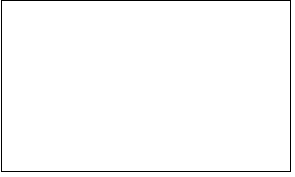
\includegraphics{grabs}
\end{graphicalabstract}

%%Research highlights
\begin{highlights}
\item Complete basis $\mathcal{P}^1$ removes the derivative aliasing mechanism of $\mathcal{L}^1$.
\item Overcomes the $\mathcal{O}(1)$ curl error plateau, recovering $\mathcal{O}(h)$ asymptotic convergence.
\item Automated scale-dependent support selection stabilizes stencils on irregular clouds.
\item Numerical verification confirms local Whitney dual equivalence and bounded stencil conditioning.
\item Spectral cavity validation and Edge FEM benchmark confirm spectral purity and convergence.
\end{highlights}

%% Keywords
\begin{keyword}
%% keywords here, in the form: keyword \sep keyword
Meshless methods \sep Vector Nodal Meshless Method (VNMM) \sep $H(\mathrm{curl})$ approximation \sep Spurious modes \sep Resonant cavities \sep Electromagnetics
%% PACS codes here, in the form: \PACS code \sep code

%% MSC codes here, in the form: \MSC code \sep code
%% or \MSC[2008] code \sep code (2000 is the default)

\end{keyword}

\end{frontmatter}

%% Add \usepackage{lineno} before \begin{document} and uncomment 
%% following line to enable line numbers
%% \linenumbers

%% main text
%%
% --- SEÇÃO 1: INTRODUÇÃO ---
\section{Introduction}
\label{sec:intro}

This section provides the contextual framework, fundamental motivations, and key scientific challenges that drive the development of advanced meshless methods for computational electromagnetics. First, the historical evolution and practical advantages of meshless paradigms over traditional grid-based methods are outlined. Subsequently, the mathematical bottlenecks of earlier vector meshless formulations---specifically derivative stagnation and support instability---are detailed, highlighting the necessity for the stabilized Vector Nodal Meshless Method (VNMM 2D) proposed in this work.

% ---------------------------------------------------------
% SUBSECTION 1.1: CONTEXT AND MOTIVATION
% ---------------------------------------------------------
\subsection{Context and Motivation}
\label{subsec:context_motivation}

The mathematical modeling of electromagnetic phenomena governed by Maxwell's partial differential equations plays a pivotal role in modern science and engineering applications \cite{jin2014finite, harrington2001time}. Because exact analytical solutions are strictly restricted to canonical geometries and homogeneous media, numerical discretization methods have become indispensable tools for simulating complex electromagnetic devices, waveguiding structures, and resonant cavities \cite{jin2014finite, monk2003finite}.

Historically, spatial discretization in computational electromagnetics (CEM) originated with finite difference techniques, notably Yee's staggered Finite-Difference Time-Domain (FDTD) grid \cite{yee1966numerical}, and the conventional node-based scalar Finite Element Method (FEM) \cite{jin2014finite}. In node-based FEM formulations, vector field variables (such as the electric field $\vec{E}$ or magnetic field $\vec{H}$) are discretized by assigning independent scalar degrees of freedom (DoFs) to each Cartesian component ($E_x, E_y, E_z$) at shared mesh vertices \cite{jin2014finite, bossavit1990spurious}. While highly successful for scalar Helmholtz and Poisson problems, applying node-based scalar approximations directly to vector Maxwell equations leads to fundamental mathematical pathologies \cite{bossavit1990spurious, boffi1999computational}:
\begin{enumerate}
    \item \textbf{Violation of Tangential Interface Continuity:} Physical vector fields across dielectric or magnetic material boundaries require continuous tangential components ($\mathbf{n} \times [\vec{E}] = \mathbf{0}$) while allowing normal components to jump discontinuously  \cite{jin2014finite, monk2003finite}. Node-based scalar shape functions enforce $C^0$ continuity across all vector components simultaneously, artificially locking normal jumps or under-specifying tangential continuity \cite{bossavit1990spurious}.
    \item \textbf{Field Singularities at Sharp Edges:} Node-based approximations fail to correctly capture singular field behavior near sharp conducting re-entrant corners and edges \cite{monk2003finite, boffi1999computational}.
    \item \textbf{Spectral Contamination by Spurious Modes:} Continuous scalar approximations do not satisfy the exact discrete de Rham complex property ($\operatorname{Im}(\nabla) \subset \ker(\nabla \times)$) \cite{monk2003finite, bossavit1990spurious}. Consequently, the infinite-dimensional nullspace of irrotational gradient fields ($\vec{E} = \nabla \phi$) leaks into the physical discrete spectrum, generating non-physical, highly oscillatory \emph{spurious modes} interspersed among true physical resonances \cite{bossavit1990spurious, boffi1999computational}.
\end{enumerate}

To overcome these severe flaws, N\'ed\'elec \cite{nedelec1980mixed} introduced mixed vector finite elements---commonly designated as Whitney 1-forms or Edge Finite Element Methods (EFEM) \cite{monk2003finite, bossavit1998computational}. As extensively detailed by Bossavit \cite{bossavit1998computational}, by associating degrees of freedom with line integrals of field circulation $e_k = \int_{E_k} \vec{E} \cdot d\boldsymbol{\ell}$ along element edges rather than scalar nodal points, EFEM constructs vector shape functions natively conforming in the Sobolev space $H(\mathbf{curl}; \Omega)$. EFEM naturally satisfies tangential interface continuity, models edge field singularities, and preserves the discrete de Rham sequence, completely eliminating spurious modes from electromagnetic spectrum calculations \cite{monk2003finite, bossavit1990spurious, bossavit1998computational}.

Despite the undeniable success of EFEM, all mesh-based formulations remain heavily burdened by the pre-requisite of generating high-quality 3D conformal meshes \cite{idelsohn2006mesh, liu2009mesh}. For problems involving complex CAD geometries, moving interfaces (such as rotating electrical machinery), severe spatial deformations, or adaptive mesh refinement, the computational overhead of mesh generation, remeshing, and element distortion repair represents a major bottleneck \cite{idelsohn2006mesh, liu2009mesh, slak2018refined}.

To liberate numerical solvers from topological mesh constraints, \emph{Meshless (or Meshfree) Methods} emerged as a powerful computational paradigm in solid mechanics, fluid dynamics, and thermodynamics \cite{liu2009mesh, liu2005introduction, atluri2002meshless}. By constructing field approximations directly over arbitrary clouds of points without pre-arranged element connectivity, meshless methods eliminate mesh generation costs and facilitate seamless adaptive node insertion \cite{liu2009mesh, belytschko1994element}. Prominent weak-form meshless paradigms include the Element-Free Galerkin (EFG) method \cite{belytschko1994element}, based on Moving Least Squares (MLS) approximations over background quadrature cells; the Meshless Local Petrov-Galerkin (MLPG) method \cite{atluri1998new, atluri2002meshless}, utilizing local quadrature subdomains to achieve a ``truly meshless'' formulation; the Point Interpolation Method (PIM) and Radial Point Interpolation Method (RPIM) \cite{liu2001point, liu2005introduction}; Smoothed Particle Hydrodynamics (SPH) \cite{monaghan1992smoothed}; and the Reproducing Kernel Particle Method (RKPM) \cite{liu2009mesh}.

Meshless formulations have demonstrated significant advantages over traditional grid-based methods in low-frequency electromagnetics, particularly for modeling deforming domains, moving boundaries, and transient phenomena in electrical machines without requiring complex remeshing procedures \cite{viana1999moving, parreira2006element, coppoli2012induction}. Early attempts to adapt meshless techniques to computational electromagnetics---such as MLS-RKPM formulations \cite{viana1999moving}, EFG schemes \cite{cingoski1998element, parreira2006element}, and MLPG vector formulations \cite{atluri2002meshless,fonseca2008imposing, nicomedes2012meshless}---primarily constructed scalar meshless shape functions for individual vector components ($E_x, E_y, E_z$). However, treating vector components independently inherited all the historical pathologies of scalar node-based FEM: appearance of non-physical spurious modes, difficult imposition of tangential interface conditions across material discontinuities, and inflated system matrix dimensions requiring auxiliary divergence-free constraints or Lagrange multipliers \cite{nicomedes2015mixed, lima2016metodos, ortiz2023tese}.

To establish a truly $H(\mathbf{curl})$-conforming meshless vector framework, Lima and Mesquita \cite{lima2017edge} developed the \emph{Edge Meshless Method} (EMM). The EMM distributes directed spatial line segments (edges) throughout the domain and constructs vector shape functions based on $H(\mathbf{curl})$ space properties \cite{lima2017edge, lima2016metodos}. 

Serving as a crucial bridge toward higher-order vector meshless representations, Silva, Mesquita, and Lima \cite{silva2018new} introduced $H(\mathbf{curl})$-conforming vector shape functions for the EMM based on N\'ed\'elec's incomplete solenoidal $\mathcal{L}^1$ polynomial space \cite{nedelec1980mixed}. By refining local circulation projections along support edges, their formulation ensured exact tangential field continuity across material interfaces, divergence-free behavior, and complete suppression of spurious modes. Building upon these vectorial shape function concepts, Ortiz et al. \cite{ortiz2021creating, ortiz2021nodal, ortiz2023tese} established higher-order expansions and investigated the asymptotic limit as physical edge lengths shrink to zero ($L_k \to 0$), giving rise to the Vector Nodal Meshless Method (VNMM 2D).

In VNMM, the 1D continuous edge degenerates into a point-collocated vector node $(P_i, \vec{t}_i)$, where each node $P_i$ is assigned a unit vector director $\vec{t}_i$ \cite{ortiz2021nodal, ortiz2023tese}. On physical boundaries and material interfaces, $\vec{t}_i$ is aligned strictly tangent to the boundary, enabling direct, unconstrained imposition of essential PEC conditions and tangential field continuity \cite{ortiz2021nodal, goncalves2025tese}. By associating a single scalar directional projection DoF ($c_i = \vec{E}(P_i) \cdot \vec{t}_i$) with each node, VNMM combines the lightweight single-DoF-per-node efficiency of scalar meshless methods with the local $H(\mathbf{curl})$ vector regularity inspired by Whitney edge elements \cite{ortiz2021nodal, goncalves2023vector, goncalves2025tese}. When nodes and directors align with the midpoints and edges of a conforming simplicial triangulation, the VNMM reproduces Whitney 1-forms exactly, inheriting global $H(\mathbf{curl})$ conformity. On arbitrary, unconstrained point clouds, however, the formulation operates as a non-conforming approximation composed of locally regular vector polynomials across dynamically chosen supports. Subsequent developments extended the VNMM to three-dimensional vector problems \cite{goncalves2023vector, goncalves2025tese} and periodic electromagnetic structures \cite{goncalves2026periodic}.

In the broader context of contemporary meshless methods widely investigated in engineering analysis and computational physics---ranging from weak-form formulations such as EFG/MLS \cite{belytschko1994element} and MLPG \cite{atluri1998new, atluri2002meshless} to strong-form/collocation strategies including RPIM \cite{liu2001point, liu2005introduction}, radial basis function-generated finite differences (RBF-FD), and generalized meshless finite differences \cite{slak2018refined}---vector field approximation has traditionally relied on uncoupled Cartesian component decomposition ($E_x, E_y$). While modern RBF-FD and local Petrov-Galerkin schemes exhibit high algebraic flexibility and high-order derivative approximations on arbitrary stencils, applying them to vector Maxwell problems requires artificial divergence cleaning, ghost-node stabilization, or auxiliary Lagrange multipliers to enforce tangential interface continuity without normal locking or spurious spectral contamination \cite{nicomedes2015mixed, slak2018refined}. Conversely, earlier vectorial meshless frameworks attempting native $H(\mathbf{curl})$ conformity---such as the Edge Meshless Method (EMM) \cite{lima2017edge} and the original $\mathcal{L}^1$ VNMM \cite{ortiz2021nodal}---relied either on finite 1D spatial segments or incomplete polynomial subspaces ($\mathcal{L}^1$), suffering from topological background dependencies or catastrophic $\mathcal{O}(1)$ derivative stagnation on unconstrained point distributions. This delineates the specific novelty gap filled by the proposed VNMM $\mathcal{P}^1 = \mathcal{P}_1 \times \mathcal{P}_1$ formulation. What the VNMM brings over scalar-component MLS, RPIM, and RBF-FD paradigms is a lean kinematic structure of \emph{one scalar DoF per node} collocated with a \emph{vector director}, providing a \emph{natural representation of tangential continuity} along physical interfaces and PEC boundaries without auxiliary constraints. Furthermore, unlike prior $H(\mathbf{curl})$ meshless attempts, the complete $\mathcal{P}^1$ formulation provides an \emph{explicit vector-polynomial structure} with a provable \emph{direct connection to Whitney 1-forms} on simplicial topologies, while delivering a \emph{curl-consistent complete Jacobian representation} that systematically eliminates derivative modal aliasing on arbitrary, mesh-free point distributions.

To synthesize these fundamental distinctions and contextualize the VNMM within the broader landscape of computational electromagnetics and meshless research \cite{liu2009mesh, belytschko1994element, atluri2002meshless, slak2018refined}, Table~\ref{tab:meshless_comparison} summarizes the mathematical and algorithmic characteristics of prominent grid-based and meshless schemes, contrasting their variable representations, interface continuities, spurious-mode control mechanisms, and curl convergence behaviors.

\begin{table}[!htbp]
\centering
\footnotesize
\setlength{\tabcolsep}{3pt}
\caption{Conceptual comparison of spatial discretization paradigms in computational electromagnetics.}
\label{tab:meshless_comparison}
\begin{tabularx}{\linewidth}{@{}
>{\raggedright\arraybackslash}p{0.18\linewidth}
>{\centering\arraybackslash}p{0.12\linewidth}
>{\centering\arraybackslash}p{0.15\linewidth}
>{\centering\arraybackslash}p{0.15\linewidth}
>{\centering\arraybackslash}p{0.18\linewidth}
>{\centering\arraybackslash}X
@{}}
\toprule
\textbf{Discretization Method} & 
\textbf{Mesh Connectivity} & 
\textbf{Field Variable Representation} & 
\textbf{$H(\mathbf{curl})$ Interface Continuity} & 
\textbf{Spurious-Mode Control Mechanism} & 
\textbf{Curl Operator Convergence on Point Clouds} \\
\midrule
\textbf{Edge FEM (EFEM)} \cite{nedelec1980mixed, monk2003finite} & 
Conformal mesh & 
Edge circulation $e_k = \int_{E_k} \vec{E} \cdot d\boldsymbol{\ell}$ & 
Natively conforming ($\mathbf{n} \times [\vec{E}] = \mathbf{0}$) & 
Exact discrete de Rham complex & 
$\mathcal{O}(h^1)$ (simplex-based) \\
\addlinespace
\textbf{Scalar EFG / MLS} \cite{belytschko1994element, cingoski1998element} & 
None (Point cloud) & 
Component splitting ($E_x, E_y$) & 
Artificial ($C^0$ normal locking / penalty) & 
Auxiliary divergence penalty or projection & 
$\mathcal{O}(h^p)$ (high-order scalar MLS) \\
\addlinespace
\textbf{Vector MLPG} \cite{atluri2002meshless, nicomedes2012meshless} & 
None (Local subdomains) & 
Component splitting ($E_x, E_y$) & 
Lagrange multipliers / penalty & 
Divergence-free projection / penalty & 
$\mathcal{O}(h^p)$ (local MLS integration) \\
\addlinespace
\textbf{RBF-FD / RPIM} \cite{liu2005introduction, slak2018refined} & 
None (Point cloud) & 
Component splitting ($E_x, E_y$) & 
Collocation / ghost node penalty & 
Divergence cleaning / penalty & 
$\mathcal{O}(h^p)$ (radial basis differentiation) \\
\addlinespace
\textbf{Original VNMM ($\mathcal{L}^1$)} \cite{ortiz2021nodal, ortiz2023tese} & 
Planar / Delaunay subdivision & 
Pointwise projection $c_k = \vec{E}(P_k) \cdot \vec{t}_k$ & 
Natural tangential director alignment & 
Conditional (restricted to structured supports) & 
$\mathcal{O}(1)$ stagnation on arbitrary clouds \\
\addlinespace
\textbf{Proposed VNMM ($\mathcal{P}^1$)} & 
None (Arbitrary point clouds) & 
Pointwise projection $c_k = \vec{E}(P_k) \cdot \vec{t}_k$ & 
Natural tangential director alignment & 
Div-curl Ritz-Galerkin penalty ($s_{\mathrm{div}} = 6.0$) & 
Consistent $\mathcal{O}(h^1)$ via full Jacobian space \\
\bottomrule
\end{tabularx}
\end{table}

% ---------------------------------------------------------
% SUBSECTION 1.2: THE CURL STAGNATION BOTTLENECK IN ARBITRARY SUPPORTS
% ---------------------------------------------------------
\subsection{The Curl Stagnation Bottleneck in Arbitrary Supports}
\label{subsec:curl_stagnation_bottleneck}

Despite the mathematical elegance of the original Vector Nodal Meshless Method (VNMM 2D) \cite{ortiz2021nodal, ortiz2023tese}, early formulations were fundamentally tied to structured support selection strategies. In foundational studies \cite{ortiz2021nodal, ortiz2023tese, goncalves2023vector}, candidate support triads $\{P_k, \vec{t}_k\}_{k=1}^3$ were constructed by referencing background spatial structures, such as macro-element planar subdivisions or Delaunay triangulations. While effective for canonical geometries, relying on underlying meshes contradicts the core ``meshless'' promise of unconstrained point-cloud discretization \cite{liu2009mesh, goncalves2025tese}.

When attempting to liberate the VNMM from spatial meshes by performing automated nearest-neighbor searches (e.g., $k$-d tree queries) over arbitrary unstructured point clouds, a severe mathematical limitation emerges: \textbf{for the arbitrary point-cloud collocation setting investigated here, the numerical approximation of the curl operator $(\nabla \times \vec{E}^h)_z$ fails to converge, exhibiting an $\mathcal{O}(1)$ relative error plateau under spatial grid refinement} \cite{goncalves2025tese}.

Unlike Edge Finite Element Methods (EFEM), where boundary line circulation integrals enforce closed-contour flux cancellation via Stokes' theorem \cite{nedelec1980mixed, monk2003finite}, point-collocated meshless schemes rely on discrete pointwise projections \cite{goncalves2025tese}. In the classical 3-node solenoidal basis $\mathcal{L}^1$, polynomial incompleteness prevents local shape functions from resolving diagonal (dilatational) gradient components ($\partial E_x/\partial x$, $\partial E_y/\partial y$). Under pointwise collocation on unstructured node distributions, unrepresented gradient components generate truncation residuals that interact with the inverted local moment placement matrix, leaking directly into the field curl calculation as an $\mathcal{O}(1)$ modal aliasing noise floor under refinement \cite{li2007meshfree, liu2009mesh}.

A complete, step-by-step mathematical derivation of this modal aliasing mechanism---including the local Taylor series Jacobian decomposition and remainder error scaling---is presented in detail in Section~\ref{subsec:L1_aliasing_analysis}.

% ---------------------------------------------------------
% SUBSECTION 1.3: SCOPE AND MAIN CONTRIBUTIONS
% ---------------------------------------------------------
\subsection{Scope and Main Contributions of the Paper}
\label{subsec:scope_contributions}
This paper presents a stabilized Vector Nodal Meshless Method (VNMM 2D) designed for robust and accurate vector field approximations on arbitrary point clouds without mesh connectivity. The core methodological contributions of this work are threefold:

\begin{enumerate}
    \item \textbf{Elimination of Modal Aliasing via Complete $\mathcal{P}^1$ Vector Basis:} 
    Transitioning from the incomplete 3-term solenoidal space $\mathcal{L}^1$ to the complete linear polynomial vector space $\mathcal{P}^1 = \mathcal{P}_1 \times \mathcal{P}_1$ ($M_{\mathrm{supp}} = 6$) resolves all four independent spatial components of the local Taylor Jacobian tensor $\mathbf{J}^h = \nabla \vec{E}^h$. As formulated in Section~\ref{subsec:complete_P1_basis} following the aliasing diagnosis in Section~\ref{subsec:L1_aliasing_analysis}, this complete representation eliminates the derivative truncation mechanism that causes the $\mathcal{O}(1)$ curl stagnation plateau in point-collocated meshless stencils.

    \item \textbf{Scale-Dependent Support Selection with Absolute Determinant Floor:} 
    To enable robust, mesh-free operation on unstructured node distributions, we establish a geometric singularity classification in $\mathbb{R}^{6\times6}$ (Sections~\ref{subsec:singularities_L1} and \ref{subsec:singularities_P1}) and propose an automated 4-phase support selection algorithm combining $k$-d tree spatial queries with scale-dependent determinant thresholding ($[\det(\mathbf{A}_{6\times6})] = [L]^4$) and an absolute tolerance floor ($\operatorname{Tol}_{\mathrm{floor}} = 1.5 \times 10^{-5}$) (Section~\ref{sec:conditioning}), filtering ill-conditioned stencils without background triangulation.

    \item \textbf{Rigorous Local Dual Equivalence Proof:} 
    We establish the Local Dual Equivalence Theorem (Section~\ref{subsubsec:formal_proof_dual_whitney}), proving that under conforming simplicial midpoints and edge directors, the local VNMM shape functions are algebraically and topologically isomorphic to lowest-order Whitney 1-forms, providing a rigorous mathematical bridge connecting nodal meshless formulations to classical Edge FEM.
\end{enumerate}

To rigorously assess these contributions and delineate the operational performance of the stabilized VNMM, the numerical campaign in Section~\ref{sec:numerical_results} is structured into three complementary stages:
\begin{itemize}
    \item \textbf{Numerical Verification Stage (Sections~\ref{subsec:conforming_dual_equivalence}--\ref{subsec:stochastic_perturbations}):} 
    First, single-simplex interpolation verifies the exact isomorphism of the Local Dual Equivalence Theorem against Whitney edge elements down to machine precision ($\approx 10^{-16}$). Second, benchmarks on arbitrary point clouds demonstrate that the complete $\mathcal{P}^1$ basis eliminates derivative aliasing, restoring first-order asymptotic curl convergence ($\mathcal{O}(h^{0.97}) \approx \mathcal{O}(h^1)$) alongside an observed superconvergent rate of $\mathcal{O}(h^{2.17})$ for the electric field on the tested $TE_{11}$ benchmark ($19.8\times$ precision gain and $25.9\times$ curl error reduction on the finest mesh). Third, a representative stochastic stress test under $25\%$ spatial jitter and random director orientations confirms that scale-dependent thresholding bounds placement matrix conditioning in the tested realization ($\kappa_2(\mathbf{A}) \le 73$ at the operational baseline floor $\operatorname{Tol}_{\mathrm{floor}} = 1.5 \times 10^{-5}$, reaching $\approx 64$ at the compromise threshold $\mathrm{Tol}_{\mathrm{det}} = 3.0 \times 10^{-5}$) and restores monotonic error reduction along the evaluated benchmark sequence.

    \item \textbf{Physics-Based Spectral Validation Stage (Sections~\ref{subsec:cavity_eigenvalues}--\ref{subsec:convergence_comparison}):} 
    First, the formulation is applied to 2D transverse electric ($TE_z$) electromagnetic resonant cavity eigenvalue problems, showing that a Ritz-Galerkin weak form with div-curl penalty regularization ($s_{\mathrm{div}} = 6.0$) shifts spurious gradient nullspace modes outside the operational band in the tested setup ($\lambda > 50$), yielding clean modal pairing with an average wavenumber error of $1.00\%$. Second, a convergence benchmark against canonical Edge FEM across six successive refinement levels reveals an observed fitted slope of $\mathcal{O}(h_{\mathrm{DoF}}^{2.80})$ over the tested refinement interval (compared to $\mathcal{O}(h_{\mathrm{DoF}}^{1.93})$ for Edge FEM), closing the coarse-grid accuracy gap with edge elements without volumetric mesh connectivity.

    \item \textbf{Methodological Scope and Limitations (Section~\ref{subsec:limitations_scope}):} 
    To establish transparent methodological boundaries, we analyze background quadrature dependencies, local stencil combinatorial complexity, point-cloud anisotropy, and penalty parameter sensitivity.
\end{itemize}

The remainder of this paper is organized as follows: Section~\ref{sec:formulations} details the 2D VNMM vector shape function construction for $\mathcal{L}^1$ and $\mathcal{P}^1$ spaces and proves the Local Dual Equivalence Theorem; Section~\ref{sec:conditioning} analyzes local placement matrix singularities and formulates the support selection algorithm; Section~\ref{sec:variational_formulation} presents the div-curl regularized weak form and point-based EFG Gauss quadrature; Section~\ref{sec:numerical_results} presents the numerical verification, spectral validation, and operational scope; and Section~\ref{sec:conclusion} concludes the paper with future research perspectives.

% --- SEÇÃO 2: FORMULAÇÃO MATEMÁTICA ---
\section{Mathematical Formulations of the 2D VNMM}
\label{sec:formulations}

This section establishes the foundational mathematical and functional framework of the two-dimensional Vector Nodal Meshless Method (VNMM 2D). It details the vector projection properties, field continuity enforcement, and the construction of local vector shape functions. First, the single-degree-of-freedom nodal projection scheme and the exact imposition of physical boundary conditions are defined. Next, the traditional incomplete $\mathcal{L}^1$ solenoidal space is reviewed, proving its exact topological and algebraic local dual equivalence with classical Whitney 1-form edge finite elements on simplicial cells. Finally, the complete linear polynomial vector space $\mathcal{P}^1$ is introduced to resolve all components of the local Taylor Jacobian tensor and eliminate derivative modal aliasing in unconstrained node clouds.

\subsection{Nodal Projection and Tangential Continuity}
\label{subsec:nodal_projection}

The Vector Nodal Meshless Method (VNMM 2D) \cite{ortiz2021nodal, ortiz2023tese} constructs local $H(\mathrm{curl})$-regular vector approximations by distributing a set of $M$ nodes throughout the computational domain $\Omega$ and its boundaries $\partial\Omega$. Unlike traditional scalar meshless formulations that assign separate degrees of freedom to individual spatial components (e.g., $E_x$ and $E_y$), the VNMM associates a single physical unit vector director $\vec{t}_i = [t_{ix}, t_{iy}]^T$ with each node $i$.

The approximate vector field $\vec{E}^h(\mathbf{x})$ at any spatial location $\mathbf{x} = (x, y) \in \Omega$ is expressed as a linear combination of vector nodal shape functions $\vec{N}_i(\mathbf{x})$:
\begin{equation}
\vec{E}^h(x, y) = \sum_{i=1}^{M_{\text{supp}}} \vec{N}_i(x, y) e_i
\label{eq:field_approx_vnmm}
\end{equation}
where $M_{\text{supp}}$ is the number of active support nodes in the local influence domain, and $e_i$ represents the discrete scalar degree of freedom (DoF) associated with the $i$-th node. Physically, $e_i$ corresponds to the pointwise directional projection of the electric field vector along the unit vector director $\vec{t}_i$ at the node coordinate $\mathbf{x}_i = (x_i, y_i)$:
\begin{equation}
e_i = \vec{E}(\mathbf{x}_i) \cdot \vec{t}_i \quad [\text{Volts/meter}]
\label{eq:dof_projection_definition}
\end{equation}

To ensure physical consistency, local curl regularity, and direct enforcement of boundary conditions, the vector shape functions $\vec{N}_i(\mathbf{x})$ are required to satisfy the vector Kronecker delta projection property \cite{lima2017edge, ortiz2021nodal}:
\begin{equation}
\vec{N}_i(\mathbf{x}_k) \cdot \vec{t}_k = \delta_{ik} = \begin{cases} 1, & \text{if } k = i \\ 0, & \text{if } k \neq i \end{cases}
\label{eq:vector_kronecker_delta}
\end{equation}
for all nodes $k$ belonging to the local support domain. Property~\eqref{eq:vector_kronecker_delta} dictates that the shape function $\vec{N}_i$ exhibits a unit projection along its own nodal director $\vec{t}_i$ at position $\mathbf{x}_i$, while maintaining zero projection along the directors of all other surrounding support nodes.

\subsubsection{Enforcement of PEC and Material Interface Conditions}
The vector Kronecker delta property~\eqref{eq:vector_kronecker_delta} enables a straightforward, exact enforcement of essential Dirichlet boundary conditions and tangential field continuity without requiring background auxiliary meshes, penalty parameters, or Lagrange multipliers \cite{goncalves2023vector, ortiz2021nodal}.

For nodes lying on Perfect Electric Conductor (PEC) boundaries $\Gamma_{\text{PEC}}$, where the physical boundary condition requires $\hat{n} \times \vec{E} = 0$ ($\hat{n}$ being the unit normal to $\partial\Omega$), the associated vector director $\vec{t}_k$ is aligned strictly tangent to the boundary contour:
\begin{equation}
\vec{t}_k \parallel \partial\Omega \implies \hat{n}(\mathbf{x}_k) \cdot \vec{t}_k = 0
\end{equation}
Consequently, the physical requirement $\hat{n} \times \vec{E} = 0$ simplifies to setting the scalar nodal DoF directly to zero:
\begin{equation}
e_k = 0 \quad \forall k \in \Gamma_{\text{PEC}}
\label{eq:pec_dirichlet_homog}
\end{equation}

Similarly, at material interfaces $\Gamma_{\text{int}}$ separating subdomains with distinct constitutive parameters ($\epsilon_{r1} \neq \epsilon_{r2}$ or $\mu_{r1} \neq \mu_{r2}$), interface nodes are assigned unit vector directors $\vec{t}_i$ oriented tangentially to $\Gamma_{\text{int}}$. Because property~\eqref{eq:vector_kronecker_delta} locks the tangential field component to $e_i$, tangential continuity ($\vec{n} \times \vec{E}_1 = \vec{n} \times \vec{E}_2$) is inherently satisfied across adjacent local support domains, while allowing natural step discontinuities in the normal field components ($\epsilon_{r1} E_{n1} = \epsilon_{r2} E_{n2}$).

\paragraph{Local Regularity versus Global $H(\mathrm{curl})$ Conformity}
It is essential to clarify the mathematical distinction between local vector regularity and global conformity in the meshless context \cite{monk2003finite, belytschko1994element}. Within any given local support domain (the virtual macro-simplex associated with a fixed node sextet), the vector shape functions $\vec{N}_i$ are smooth polynomials and thus belong strictly to $H(\mathrm{curl})$ locally. On conforming simplicial meshes where supports coincide with cell triangles, the global assembled space is indeed $H(\mathrm{curl})$-conforming (as proven in Section~\ref{subsubsec:formal_proof_dual_whitney}). However, on arbitrary, unconstrained point clouds, the active support is determined dynamically for each evaluation point. Across the boundaries where the active support changes, the tangential trace $[\hat{n} \times \vec{E}^h]$ generally exhibits small numerical discontinuities. Consequently, the assembled global discrete space is \emph{not} globally $H(\mathrm{curl})$-conforming ($V_h \not\subset H(\mathrm{curl}; \Omega)$); rather, it is a non-conforming approximation built from local $H(\mathrm{curl})$-regular vector fields. This distinction is central to understanding both the behavior of the discrete curl operator and the necessity of variational regularization.

\subsection{The Incomplete \texorpdfstring{$\mathcal{L}^1$}{L1} Basis (3 Support Nodes)}
\label{subsec:incomplete_l1_basis}
The construction of vector shape functions in the 2D VNMM directly inherits the mathematical foundations of $H(\mathbf{curl})$-conforming edge-based meshless approximations \cite{lima2017edge, silva2018new}. The incomplete 3-term solenoidal polynomial space 
\begin{equation}
 \mathcal{L}^1 = \operatorname{span}\{ \begin{bmatrix}1\\0\end{bmatrix}, \begin{bmatrix}0\\1\end{bmatrix}, \begin{bmatrix}y\\-x\end{bmatrix} \}    
\end{equation}
corresponds to the local two-dimensional reduction of Nédélec's first-type space \cite{nedelec1980mixed}, whose vector projection mechanisms were established for edge meshless line segments by Silva et al. \cite{silva2018new} and later adapted to point-collocated nodes \cite{ortiz2021nodal, ortiz2023tese}.

Consequently, the local vector shape function $\vec{N}_i$ associated with the $i$-th support node in a 3-node local domain is defined as a linear combination of these basis vectors:
\begin{equation}
\vec{N}_i(x, y) = \beta_{1i} \begin{bmatrix} 1 \\ 0 \end{bmatrix} + \beta_{2i} \begin{bmatrix} 0 \\ 1 \end{bmatrix} + \beta_{3i} \begin{bmatrix} y \\ -x \end{bmatrix}
\label{eq:N_i_L1}
\end{equation}
where $\boldsymbol{\beta}_i = [\beta_{1i}, \beta_{2i}, \beta_{3i}]^T \in \mathbb{R}^3$ represents the unknown local interpolation coefficient vector.

To determine these coefficients, the vector shape functions are constrained to satisfy the vector Kronecker delta projection property~\eqref{eq:vector_kronecker_delta} for $i,k=1,2,3$,

Applying constraint~\eqref{eq:vector_kronecker_delta} to all three support nodes leads to the local $3 \times 3$ linear placement system: 
\begin{equation}
\mathbf{A} \boldsymbol{\beta}_i = \mathbf{L}_i
\label{eq:linear_placement_system}
\end{equation}
where the local moment placement matrix $\mathbf{A} \in \mathbb{R}^{3 \times 3}$ is explicitly given by:
\begin{equation}
\mathbf{A} = \begin{bmatrix}
t_{1x} & t_{1y} & y_1 t_{1x} - x_1 t_{1y} \\
t_{2x} & t_{2y} & y_2 t_{2x} - x_2 t_{2y} \\
t_{3x} & t_{3y} & y_3 t_{3x} - x_3 t_{3y}
\end{bmatrix}
\label{eq:matrix_A_L1}
\end{equation}
and the canonical load vectors are $\mathbf{L}_1 = [1, 0, 0]^T$, $\mathbf{L}_2 = [0,1,0]^T$, and $\mathbf{L}_3 = [0,0,1]^T$.

Once the coefficients $\boldsymbol{\beta}_i = \mathbf{A}^{-1} \mathbf{L}_i$ are evaluated, the approximated electric field vector $\vec{E}^h(x, y)$ is constructed via nodal projection superposition:
\begin{equation}
\vec{E}^h(x, y) = \sum_{i=1}^3 \vec{N}_i(x, y) e_i
\end{equation}
where $e_i = \vec{E}(\mathbf{x}_i) \cdot \vec{t}_i$ represent the discrete scalar projection DoFs.

\subsubsection{Mathematical Properties and Solenoidal Identity}
The shape functions $\vec{N}_i$ of the $\mathcal{L}^1$ basis possess two distinct mathematical characteristics:

1. \textbf{Identical Solenoidal Property ($\nabla \cdot \vec{N}_i \equiv 0$):} Taking the divergence of Eq.~\eqref{eq:N_i_L1} yields:
\begin{equation}
\nabla \cdot \vec{N}_i = \frac{\partial}{\partial x}(\beta_{1i} + \beta_{3i} y) + \frac{\partial}{\partial y}(\beta_{2i} - \beta_{3i} x) \equiv 0
\end{equation}

2. \textbf{Univariate Curl Representation:} Evaluating the scalar $z$-directed curl operator on $\vec{N}_i$ yields:
\begin{equation}
(\nabla \times \vec{N}_i)_z = \frac{\partial N_{iy}}{\partial x} - \frac{\partial N_{ix}}{\partial y} = \frac{\partial (-\beta_{3i} x)}{\partial x} - \frac{\partial (\beta_{3i} y)}{\partial y} = -2\beta_{3i}
\end{equation}
Therefore, the approximated $z$-directed scalar curl field $(\nabla \times \vec{E}^h)_z$ is spatially constant across the 3-node support domain and depends exclusively on the third coefficient $\beta_{3i}$:
\begin{equation}
(\nabla \times \vec{E}^h)_z = -2 \sum_{i=1}^3 \beta_{3i} e_i
\end{equation}

\subsubsection{Local Dual Whitney Equivalence and Constructive Isomorphism}
\label{subsubsec:dual_whitney}
The VNMM 2D was originally conceptualized as the zero-edge-length asymptotic limit of the Edge Meshless Method (EMM) \cite{lima2017edge, ortiz2021nodal}. By examining this heritage, a fundamental mathematical duality and constructive isomorphism between the VNMM point-collocation formulation and classic lowest-order Whitney edge finite elements (N\'ed\'elec 1-forms on triangular simplices \cite{nedelec1980mixed, monk2003finite}) is formally established, as detailed in Fig.~\ref{fig:whitney_vnmm_dual_equivalence}.

\begin{figure*}[!t]
\centering
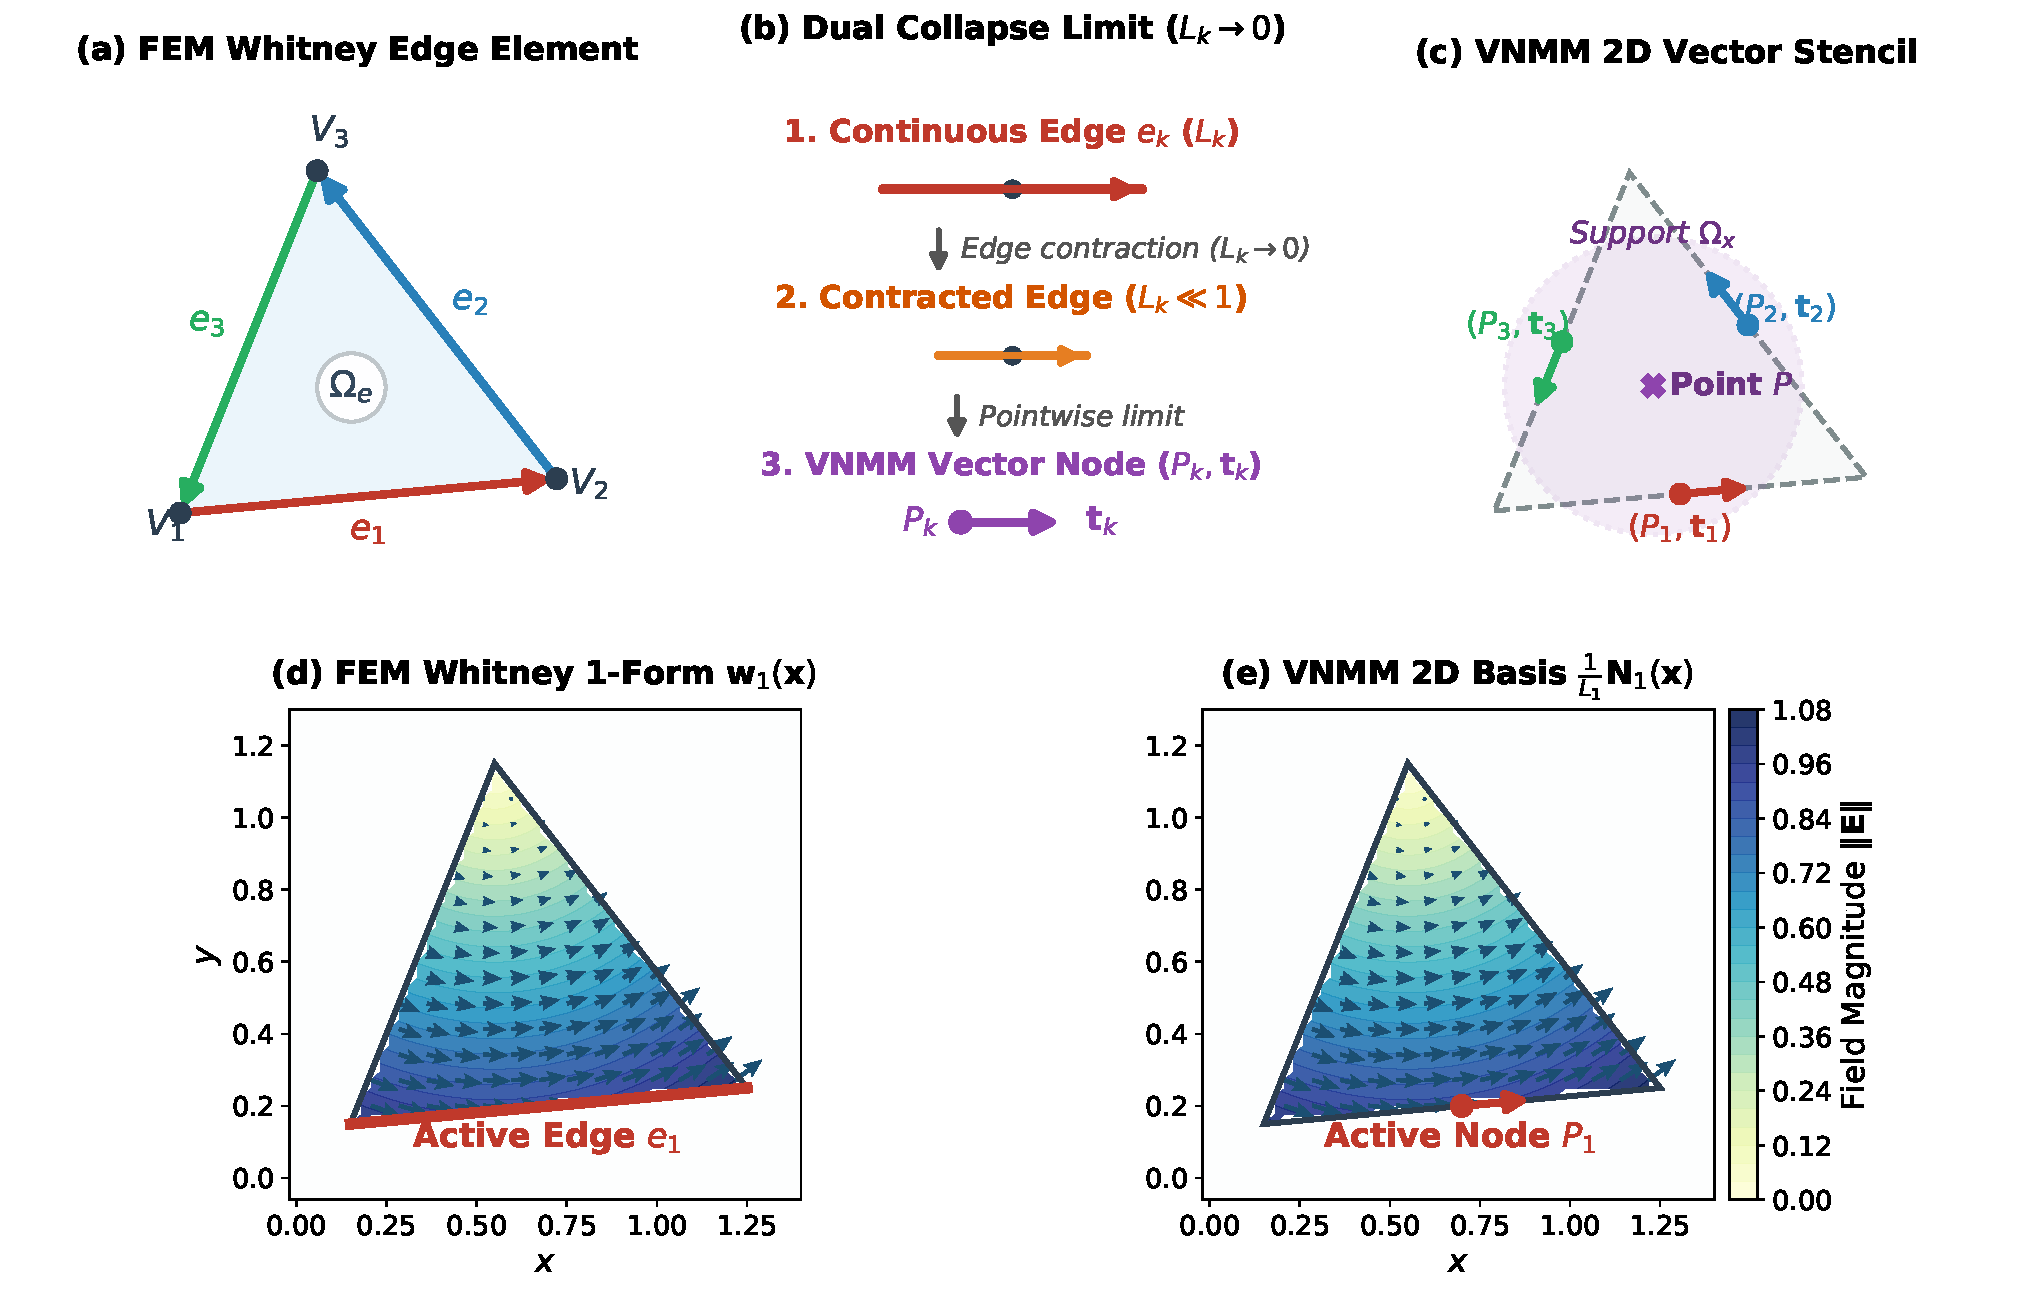
\includegraphics[width=\textwidth]{figura_equivalencia_dual_whitney_vnmm.pdf}
\caption{Exact topological and algebraic local dual equivalence between lowest-order Whitney edge elements (FEM 1-forms) and the VNMM 2D $\mathcal{L}^1$ meshless vector formulation: 
(a) Primal triangular cell $\Omega_e$ with vertices $V_1, V_2, V_3$ and oriented edges $e_1, e_2, e_3$; 
(b) Conceptual dual collapse limit as edge length contracts ($L_k \to 0$), identifying the discrete circulation integral $L_k^{-1} \int_{e_k} \vec{E}\cdot\vec{t}_k\,ds$ directly with the tangential projection at a point, $e_k = \vec{E}(P_k)\cdot\vec{t}_k$; 
(c) VNMM 2D meshless support stencil with vector nodes $(P_k, \vec{t}_k)$ placed at the edge midpoints and compact support $\Omega_x$; 
(d) Vector field and magnitude contour of the Whitney 1-form $\vec{w}_1(\mathbf{x}) = \lambda_1 \nabla\lambda_2 - \lambda_2 \nabla\lambda_1$ associated with active edge $e_1$; 
(e) Vector field and magnitude contour of the normalized VNMM $\mathcal{L}^1$ vector basis function $\frac{1}{L_1}\vec{N}_1(\mathbf{x})$ associated with active node $(P_1, \vec{t}_1)$. 
Both fields are algebraically identical over $\Omega_e$, satisfying $\|\vec{w}_1(\mathbf{x}) - L_1^{-1}\vec{N}_1(\mathbf{x})\|_{L^\infty(\Omega_e)} \le 2.2 \times 10^{-16}$.}
\label{fig:whitney_vnmm_dual_equivalence}
\end{figure*}


In conventional FEM (Fig.~\ref{fig:whitney_vnmm_dual_equivalence}a), the degrees of freedom associated with the triangular cell $\Omega_e$ are line integrals of circulation $\alpha_k = \oint_{e_k} \vec{E} \cdot d\boldsymbol{\ell}$ along continuous 1D edges of finite physical length $L_k$. As demonstrated in the asymptotic collapse limit (Fig.~\ref{fig:whitney_vnmm_dual_equivalence}b), when the physical edge length shrinks to zero ($L_k \to 0$), the 1D continuous edge degenerates into a point-collocated vector node $(P_k, \vec{t}_k)$, where the circulation DoF $\alpha_k$ naturally scales into a pointwise directional field projection $e_k = \vec{E}(P_k) \cdot \vec{t}_k$ [Volts/meter].

\subsubsection{Formal Proof of the Local Dual Equivalence Theorem}
\label{subsubsec:formal_proof_dual_whitney}
Let $T \subset \mathbb{R}^2$ be an arbitrary non-degenerate triangular simplex with vertices $V_1, V_2, V_3$ ordered counter-clockwise and non-zero area $|T| > 0$. Let $e_k = (V_k, V_{k+1})$ be the directed boundary edges of length $L_k = \|V_{k+1} - V_k\| > 0$, with unit tangent vectors $\vec{t}_k = (V_{k+1} - V_k)/L_k$ and midpoints $M_k = \frac{1}{2}(V_k + V_{k+1})$ for $k \in \{1, 2, 3\}$ (with index wrap-around $V_4 \equiv V_1$).

\begin{theorem}[Local Dual Equivalence of Whitney 1-Forms and VNMM 2D $\mathcal{L}^1$]
Consider the support triad of vector nodes $\{P_k, \vec{t}_k\}_{k=1}^3$ defined at the edge midpoints $P_k = M_k$ with directors $\vec{t}_k$. The VNMM 2D $\mathcal{L}^1$ shape functions $\vec{N}_k(\mathbf{x})$ and the Whitney 1-forms $\vec{w}_k(\mathbf{x}) = \lambda_i(\mathbf{x})\nabla\lambda_j - \lambda_j(\mathbf{x})\nabla\lambda_i$ satisfy:
\begin{equation}
\vec{N}_k(\mathbf{x}) \equiv L_k \, \vec{w}_k(\mathbf{x}) \quad \Longleftrightarrow \quad \vec{w}_k(\mathbf{x}) \equiv \frac{1}{L_k} \vec{N}_k(\mathbf{x}), \quad \forall \mathbf{x} \in \mathbb{R}^2, \ \forall k \in \{1, 2, 3\}
\label{eq:dual_equivalence_scaling}
\end{equation}
\end{theorem}

\begin{proof}
The proof proceeds in five constructive steps:

\textbf{Step 1: Isomorphism of Approximation Spaces.} 
The lowest-order Whitney space $\mathcal{W}(T)$ on $T$ is spanned by $\vec{w}_k(\mathbf{x}) = [a_1 + \alpha y, a_2 - \alpha x]^T$. By inspection of the spanning vectors, $\mathcal{W}(T) = \operatorname{span}\{[1,0]^T$, $[0,1]^T$, $[y,-x]^T\} \equiv \mathcal{L}^1$. Thus, both approximation spaces share identical 3-dimensional vector polynomial spaces.

\textbf{Step 2: Constancy of Tangential Field Projection Along Simplex Edges.} 
Let $\vec{u}(\mathbf{x}) = [a_1 + \alpha y, a_2 - \alpha x]^T \in \mathcal{L}^1$. The directional projection of $\vec{u}(\mathbf{x})$ along unit director $\vec{t}_k = [\Delta x_k / L_k, \Delta y_k / L_k]^T$ is:
\begin{equation}
\vec{u}(\mathbf{x}) \cdot \vec{t}_k = \frac{1}{L_k} \left[ a_1 \Delta x_k + a_2 \Delta y_k + \alpha (y \Delta x_k - x \Delta y_k) \right]
\end{equation}
Since any point $\mathbf{x} = (x,y)$ on edge $e_k$ satisfies $(x - x_k)\Delta y_k - (y - y_k)\Delta x_k = 0$, the rotational term $y \Delta x_k - x \Delta y_k = y_k \Delta x_k - x_k \Delta y_k$ is strictly constant along the entire edge length. Therefore, the tangential projection is invariant along $e_k$:
\begin{equation}
\vec{u}(\mathbf{x}) \cdot \vec{t}_k = \vec{u}(M_k) \cdot \vec{t}_k, \quad \forall \mathbf{x} \in e_k
\label{eq:edge_constancy}
\end{equation}

\textbf{Step 3: Reduction of Edge Circulation to Pointwise Midpoint Value.} 
Using Eq.~\eqref{eq:edge_constancy}, the line integral defining the FEM circulation degree of freedom along edge $e_j$ simplifies to:
\begin{equation}
\oint_{e_j} \vec{u} \cdot d\boldsymbol{\ell} = \int_{-L_j/2}^{L_j/2} \left( \vec{u}(\mathbf{x}(s)) \cdot \vec{t}_j \right) ds = \left( \vec{u}(M_j) \cdot \vec{t}_j \right) \int_{-L_j/2}^{L_j/2} ds = L_j \left( \vec{u}(M_j) \cdot \vec{t}_j \right)
\end{equation}
Substituting the $k$-th Whitney basis function $\vec{w}_k \in \mathcal{W}(T)$, which satisfies $\oint_{e_j} \vec{w}_k \cdot d\boldsymbol{\ell} = \delta_{jk}$ by construction, yields:
\begin{equation}
L_j \left( \vec{w}_k(M_j) \cdot \vec{t}_j \right) = \delta_{jk} \quad \implies \quad \left( L_k \vec{w}_k(M_j) \right) \cdot \vec{t}_j = \delta_{jk}
\label{eq:whitney_midpoint_proj}
\end{equation}

\textbf{Step 4: Uniqueness and Exact Identification with VNMM Shape Functions.} 
By definition of the VNMM 2D $\mathcal{L}^1$ interpolation problem on the support triad $\{M_j, \vec{t}_j\}_{j=1}^3$, the shape functions satisfy $\vec{N}_k(M_j) \cdot \vec{t}_j = \delta_{jk}$. Consider the difference field:
\begin{equation}
\vec{d}_k(\mathbf{x}) = \vec{N}_k(\mathbf{x}) - L_k \vec{w}_k(\mathbf{x}) \in \mathcal{L}^1
\end{equation}
Evaluating its projection at each midpoint $M_j$:
\begin{equation}
\vec{d}_k(M_j) \cdot \vec{t}_j = \vec{N}_k(M_j) \cdot \vec{t}_j - L_k \left( \vec{w}_k(M_j) \cdot \vec{t}_j \right) = \delta_{jk} - \delta_{jk} = 0, \quad \forall j \in \{1, 2, 3\}
\end{equation}
Because triangle $T$ is non-degenerate, the local moment placement matrix $\mathbf{A} \in \mathbb{R}^{3 \times 3}$ is non-singular ($\det \mathbf{A} \neq 0$). The only vector field in $\mathcal{L}^1$ satisfying zero projections across all three support directors is the trivial field $\vec{d}_k(\mathbf{x}) \equiv \mathbf{0}$, which proves the exact identity $\vec{N}_k(\mathbf{x}) \equiv L_k \vec{w}_k(\mathbf{x})$ everywhere in $\mathbb{R}^2$.

\textbf{Step 5: Verification of Differential Invariants.} 
1. \textit{Divergence:} For any field $\vec{u} = [a_1 + \alpha y, a_2 - \alpha x]^T \in \mathcal{L}^1$, we have $\nabla \cdot \vec{u} = \partial(a_1 + \alpha y)/\partial x + \partial(a_2 - \alpha x)/\partial y \equiv 0$. Thus, $\nabla \cdot \vec{w}_k \equiv 0$ and $\nabla \cdot \vec{N}_k \equiv 0$ everywhere.
2. \textit{Curl:} Applying Stokes' theorem over triangle $T$ for Whitney 1-form $\vec{w}_k$:
\begin{equation}
\int_T (\nabla \times \vec{w}_k)_z d\Omega = \oint_{\partial T} \vec{w}_k \cdot d\boldsymbol{\ell} = \sum_{j=1}^3 \delta_{jk} = 1 \implies (\nabla \times \vec{w}_k)_z = \frac{1}{|T|}
\end{equation}
By the scaling law~\eqref{eq:dual_equivalence_scaling}, $(\nabla \times \vec{N}_k)_z = L_k (\nabla \times \vec{w}_k)_z = L_k / |T|$.
\end{proof}

This constructive isomorphism is graphically presented in Fig.~\ref{fig:whitney_vnmm_dual_equivalence}d and~\ref{fig:whitney_vnmm_dual_equivalence}e and is verified numerically in Section~\ref{subsec:conforming_dual_equivalence}.


\subsubsection{Extension of the Valid Physical Interpolation Domain}
This local dual Whitney equivalence resolves a longstanding misconception regarding meshless vector interpolation domains \cite{goncalves2025tese}. In conventional scalar meshless methods (e.g., Moving Least Squares or Element-Free Galerkin), evaluating field approximations outside the physical convex hull enclosed by the node coordinates $\mathbf{x}_k$ constitutes an unconstrained extrapolation, leading to rapid truncation error growth \cite{lima2017edge}.

However, because the VNMM vector basis reproduces the complete polynomial space of Whitney edge elements over the virtual macro-triangle $\Omega_{x}$ defined by the intersecting dotted lines of action of vector directors $\vec{t}_k$ (Fig.~\ref{fig:whitney_vnmm_dual_equivalence}c), the valid domain for local $H(\mathrm{curl})$ field approximation and constant curl representation is not geographically restricted to the small physical convex hull of $\mathbf{x}_k$ \cite{nedelec1980mixed, monk2003finite}. Instead, as proven by the dual scaling law~\eqref{eq:dual_equivalence_scaling}, it extends throughout the entire interior bounding region of the virtual macro-triangle. 

Under the regular-support assumptions considered here, guaranteeing that the local placement matrix $\mathbf{A}$ remains well-conditioned and that intersection vertices remain bounded and non-degenerate, field evaluations at any point $P \in \Omega_{x}$ preserve local $H(\mathrm{curl})$ regularity. In this setting, the complete $\mathcal{P}^1$ vector basis provides the polynomial reproduction required for first-order derivative consistency, while the corresponding asymptotic convergence rates are subsequently verified numerically in Section~\ref{sec:numerical_results}.

\subsubsection{Mathematical Origin of Modal Aliasing and Curl Stagnation}
\label{subsec:L1_aliasing_analysis}

Despite its solenoidal identity and exact local dual equivalence to Whitney edge elements on conforming simplices, the incomplete $\mathcal{L}^1$ basis exhibits a critical limitation when transitioned to meshless point clouds. For the arbitrary point-cloud collocation setting investigated here, the $\mathcal{L}^1$ curl approximation fails to achieve asymptotic convergence under refinement, stagnating at an $\mathcal{O}(1)$ relative error plateau \cite{goncalves2025tese}. Crucially, this limitation does not imply an intrinsic defect in $\mathcal{L}^1$ as a vector space in general---as evidenced by its optimal convergence in conforming Whitney edge elements where closed-contour circulations enforce Stokes' cancellation---but rather stems from deploying an incomplete polynomial basis within a meshless pointwise collocation framework devoid of closed boundary integrals.

The mathematical origin of this derivative stagnation lies in the local Taylor series expansion of the exact electric field $\vec{E}$ centered at the evaluation point $P(x_P, y_P)$ \cite{li2007meshfree, liu2009mesh}:
\begin{equation}
\vec{E}(\mathbf{x}) = \vec{E}(P) + \mathbf{J}(P) \begin{bmatrix} \Delta x \\[2pt] \Delta y \end{bmatrix} + \mathcal{O}(h^2)
\label{eq:taylor_vector_expansion}
\end{equation}
where $\mathbf{J}(P) = \nabla \vec{E}$ represents the complete first-order field Jacobian tensor \cite{liu2009mesh}:
\begin{equation}
\mathbf{J} = \begin{bmatrix} 
\frac{\partial E_x}{\partial x} & \frac{\partial E_x}{\partial y} \\[4pt]
\frac{\partial E_y}{\partial x} & \frac{\partial E_y}{\partial y} 
\end{bmatrix}
\label{eq:jacobian_tensor_raw}
\end{equation}

By expressing individual spatial derivatives in terms of fundamental vector calculus operators---namely, the field divergence $\nabla \cdot \vec{E} = \partial E_x/\partial x + \partial E_y/\partial y$ and the z-directed field curl $(\nabla \times \vec{E})_z = \partial E_y/\partial x - \partial E_x/\partial y$---the field Jacobian tensor is decomposed as:
\begin{equation}
\mathbf{J} = \frac{1}{2}(\nabla \cdot \vec{E}) \mathbf{I} + \frac{1}{2}(\nabla \times \vec{E})_z \begin{bmatrix} 0 & -1 \\ 1 & 0 \end{bmatrix} + \begin{bmatrix} \delta_{\mathrm{norm}} & -\delta_{\mathrm{trans}} \\ \delta_{\mathrm{trans}} & -\delta_{\mathrm{norm}} \end{bmatrix}
\label{eq:jacobian_tensor_EM_decomposition}
\end{equation}
where $\delta_{\mathrm{norm}} = \frac{1}{2}(\partial E_x/\partial x - \partial E_y/\partial y)$ denotes the normal (longitudinal) field derivative difference, and $\delta_{\mathrm{trans}} = \frac{1}{2}(\partial E_y/\partial x + \partial E_x/\partial y)$ represents the symmetric transverse field derivative component.

In the incomplete $\mathcal{L}^1$ basis, local shape functions provide only 3 degrees of freedom. As a result, normal field derivatives are artificially forced to vanish identically ($\partial E_x^h/\partial x \equiv 0$ and $\partial E_y^h/\partial y \equiv 0$), imposing $\nabla \cdot \vec{E}^h \equiv 0$ and $\delta_{\mathrm{norm}} \equiv 0$ simultaneously.

This fundamental limitation is formalized in the following proposition:

\begin{proposition}[Jacobian Incompleteness and Derivative Modal Aliasing]
Let $\vec{E} \in [C^2(\Omega)]^2$ be an arbitrary twice continuously differentiable 2D vector field. The incomplete solenoidal space $\mathcal{L}^1 = \operatorname{span}\{[1, 0]^T, [0, 1]^T, [y, -x]^T\} \subset \mathcal{P}_1 \times \mathcal{P}_1$ cannot reproduce the complete first-order Taylor expansion of $\vec{E}$. Specifically, while the complete space $\mathcal{P}^1 = \mathcal{P}_1 \times \mathcal{P}_1$ possesses $\dim(\mathcal{P}^1) = 6$ degrees of freedom to reconstruct the 2 translation components and all 4 independent entries of the Jacobian tensor $\mathbf{J} = \nabla\vec{E}$, $\mathcal{L}^1$ possesses only $\dim(\mathcal{L}^1) = 3$ degrees of freedom, enforcing the artificial linear constraints:
\begin{equation}
\frac{\partial E_x^h}{\partial x} = 0, \quad \frac{\partial E_y^h}{\partial y} = 0, \quad \text{and} \quad \frac{\partial E_x^h}{\partial y} + \frac{\partial E_y^h}{\partial x} = 0.
\label{eq:L1_derivative_constraints}
\end{equation}
Consequently, under point-collocated projection on unstructured node clouds, unrepresented normal gradients ($\partial E_x/\partial x, \partial E_y/\partial y \neq 0$) generate a projection remainder $\mathbf{r} \sim \mathcal{O}(h)$ that couples into the rotational coefficient through the inverted moment placement matrix $\mathbf{A}^{-1} \sim \mathcal{O}(h^{-1})$, inducing an $\mathcal{O}(1)$ derivative aliasing error in the discrete curl operator under refinement in the collocated setting:
\begin{equation}
\|(\nabla \times \vec{E})_z - (\nabla \times \vec{E}^h)_z\|_{L^2(\Omega)} \sim \|\mathbf{A}^{-1} \mathbf{r}\| = \mathcal{O}(h^{-1}) \cdot \mathcal{O}(h) = \mathcal{O}(1).
\label{eq:aliasing_order_proof}
\end{equation}
\end{proposition}

\begin{proof}
Let any discrete vector field $\vec{E}^h \in \mathcal{L}^1$ be expanded in terms of the solenoidal basis:
\begin{equation}
\vec{E}^h(x, y) = a \begin{bmatrix} 1 \\ 0 \end{bmatrix} + b \begin{bmatrix} 0 \\ 1 \end{bmatrix} + c \begin{bmatrix} y \\ -x \end{bmatrix}, \quad a, b, c \in \mathbb{R}.
\label{eq:proof_L1_expansion}
\end{equation}
Direct differentiation with respect to spatial coordinates yields the discrete Jacobian tensor:
\begin{equation}
\mathbf{J}^h = \begin{bmatrix} 
\frac{\partial E_x^h}{\partial x} & \frac{\partial E_x^h}{\partial y} \\[4pt] 
\frac{\partial E_y^h}{\partial x} & \frac{\partial E_y^h}{\partial y} 
\end{bmatrix} = \begin{bmatrix} 
0 & c \\ 
-c & 0 
\end{bmatrix}.
\label{eq:proof_discrete_jacobian}
\end{equation}
Inspect Eq.~\eqref{eq:proof_discrete_jacobian} establishes that $\partial E_x^h/\partial x \equiv 0$, $\partial E_y^h/\partial y \equiv 0$, and $\partial E_x^h/\partial y + \partial E_y^h/\partial x = c - c \equiv 0$, identically satisfying the linear constraints in Eq.~\eqref{eq:L1_derivative_constraints}.

Now consider a general smooth physical field $\vec{E} \in [C^2(\Omega)]^2$. Its Taylor expansion centered at evaluation point $P$ is $\vec{E}(\mathbf{x}) = \vec{E}(P) + \mathbf{J}(P) \Delta\mathbf{x} + \mathcal{O}(h^2)$, where $\mathbf{J}(P)$ has non-zero diagonal entries ($\partial E_x/\partial x \neq 0$ or $\partial E_y/\partial y \neq 0$). Collocating $\vec{E}^h$ at support nodes $\mathbf{x}_k$ ($k=1,2,3$) along unit directors $\vec{t}_k$ defines the linear placement system $\mathbf{A} [a, b, c]^T = \mathbf{e}$, where $e_k = \vec{E}(\mathbf{x}_k) \cdot \vec{t}_k$.

Subtracting the projection of the unrepresented linear components $(\mathbf{J}(P) - \mathbf{J}^h) \Delta\mathbf{x}_k \cdot \vec{t}_k$ yields a nodal projection residual $\mathbf{r} \in \mathbb{R}^3$ with asymptotic magnitude $\|\mathbf{r}\| \sim \mathcal{O}(h)$. In the $3 \times 3$ moment placement matrix $\mathbf{A}$ (Eq.~\eqref{eq:matrix_A_L1}), translation columns 1--2 scale as $\mathcal{O}(1)$, while the rotational moment column 3 scales as $(\Delta y_k t_{kx} - \Delta x_k t_{ky}) \sim \mathcal{O}(h)$. Consequently, by Cramer's rule or Neumann inversion, the third row of $\mathbf{A}^{-1}$ (which maps nodal data to the rotational DoF $c = -\frac{1}{2}(\nabla \times \vec{E}^h)_z$) scales strictly as $\|\operatorname{Row}_3(\mathbf{A}^{-1})\| \sim \mathcal{O}(h^{-1})$.

The numerical error in the reconstructed curl is therefore governed by the propagation of the projection remainder:
\begin{equation}
\begin{aligned}
|(\nabla \times \vec{E})_z - (\nabla \times \vec{E}^h)_z| &= 2 |c_{\mathrm{exact}} - c| \\
&\sim \|\operatorname{Row}_3(\mathbf{A}^{-1})\| \|\mathbf{r}\| = \mathcal{O}(h^{-1}) \cdot \mathcal{O}(h) = \mathcal{O}(1),
\end{aligned}
\end{equation}
which is independent of $h$ and generates the $\mathcal{O}(1)$ stagnation plateau in the tested collocated setting, completing the proof.
\end{proof}

\begin{table}[!htbp]
\centering
\caption{Comparison of polynomial completeness, dimensionality, and derivative reproduction capabilities between the incomplete solenoidal space $\mathcal{L}^1$ and the complete linear vector polynomial space $\mathcal{P}^1$.}
\label{tab:basis_completeness_comparison}
\resizebox{\columnwidth}{!}{%
\begin{tabular}{@{} l c c c c c c @{}}
\toprule
\textbf{Vector Space} & $\dim$ & $E_x, E_y$ & $\partial E_x/\partial x$ & $\partial E_x/\partial y$ & $\partial E_y/\partial x$ & $\partial E_y/\partial y$ \\
\midrule
$\mathcal{L}^1$ (Incomplete solenoidal) & 3 & \checkmark & \texttimes & \checkmark & \checkmark & \texttimes \\
$\mathcal{P}^1 = \mathcal{P}_1 \times \mathcal{P}_1$ (Complete linear) & 6 & \checkmark & \checkmark & \checkmark & \checkmark & \checkmark \\
\bottomrule
\end{tabular}%
}
\end{table}

In Edge Finite Element Methods (EFEM), this lack of explicit normal derivative representation does not cause stagnation because continuous line circulation integrals along element edges enforce closed-contour flux cancellation via Stokes' theorem \cite{nedelec1980mixed, monk2003finite}. In the VNMM, however, continuous line integrals are replaced by discrete pointwise projections \cite{goncalves2025tese}. Consequently, the $\mathcal{O}(1)$ derivative noise floor established in Proposition~1 cannot be eliminated by spatial mesh refinement alone ($h \to 0$). Adopting the complete linear polynomial vector space $\mathcal{P}^1 = \mathcal{P}_1 \times \mathcal{P}_1$, as formulated in Section~\ref{subsec:complete_P1_basis}, provides a direct and sufficient remedy by resolving the complete local Jacobian and eliminating this specific derivative-aliasing mechanism on unconstrained point clouds.


% ---------------------------------------------------------
% SUBSECTION 2.3: THE COMPLETE P1 VECTOR POLYNOMIAL BASIS
% ---------------------------------------------------------
\subsection{The Complete \texorpdfstring{$\mathcal{P}^1$}{P1} Vector Polynomial Basis}
\label{subsec:complete_P1_basis}

To eliminate the derivative modal aliasing and curl stagnation inherent to the incomplete $\mathcal{L}^1$ space, we reformulate local vector interpolation using the complete linear polynomial vector space $\mathcal{P}^1 = \mathcal{P}_1 \times \mathcal{P}_1$. This transition draws a direct mathematical analogy to Nédélec's second family of mixed finite elements \cite{nedelec1986new}, in which vector field approximations are constructed over complete polynomial spaces $(\mathbb{P}_k)^d$ rather than solenoidal-restricted subspaces.

In two dimensions ($d=2$), a complete first-order vector polynomial basis $\mathcal{P}^1$ provides 6 independent degrees of freedom ($M_{\mathrm{supp}} = 6$ support nodes per evaluation point):
\begin{equation}
\mathcal{P}^1 = \operatorname{span} \left\{ 
\begin{bmatrix} 1 \\ 0 \end{bmatrix}, 
\begin{bmatrix} 0 \\ 1 \end{bmatrix}, 
\begin{bmatrix} x \\ 0 \end{bmatrix}, 
\begin{bmatrix} y \\ 0 \end{bmatrix}, 
\begin{bmatrix} 0 \\ x \end{bmatrix}, 
\begin{bmatrix} 0 \\ y \end{bmatrix} 
\right\}
\label{eq:complete_P1_basis_vectors}
\end{equation}

Using this complete basis, the local vector shape function $\vec{N}_i(\mathbf{x})$ associated with the $i$-th support node is expressed as a linear combination of its six constituent terms:
\begin{equation}
\vec{N}_i(x, y) = \beta_{1i} \begin{bmatrix} 1 \\ 0 \end{bmatrix} + \beta_{2i} \begin{bmatrix} 0 \\ 1 \end{bmatrix} + \beta_{3i} \begin{bmatrix} x \\ 0 \end{bmatrix} + \beta_{4i} \begin{bmatrix} y \\ 0 \end{bmatrix} + \beta_{5i} \begin{bmatrix} 0 \\ x \end{bmatrix} + \beta_{6i} \begin{bmatrix} 0 \\ y \end{bmatrix}
\label{eq:P1_shape_function_expansion}
\end{equation}
where $\beta_{ji}$ (for $j=1, \dots, 6$) represent the local interpolation coefficients to be determined.

Enforcing the vector Kronecker delta projection property \cite{ortiz2021nodal}:
\begin{equation}
\vec{N}_i(\mathbf{x}_k) \cdot \vec{t}_k = \delta_{ik}, \quad \text{for } k = 1, \dots, 6
\label{eq:kronecker_projection_P1}
\end{equation}
across all six support nodes yields the local linear placement system 
\begin{equation}
\mathbf{A} \boldsymbol{\beta}_i = \mathbf{L}_i. 
\label{eq:linear_system_P1}
\end{equation}
Evaluated in local translated coordinates centered at the evaluation point $P(x_P, y_P)$ (defined as $\Delta x_k = x_k - x_P$ and $\Delta y_k = y_k - y_P$), the local moment placement matrix $\mathbf{A} \in \mathbb{R}^{6 \times 6}$ is explicitly given by:
\begin{equation}
\mathbf{A} = \begin{bmatrix}
t_{1x} & t_{1y} & \Delta x_1 t_{1x} & \Delta y_1 t_{1x} & \Delta x_1 t_{1y} & \Delta y_1 t_{1y} \\[4pt]
t_{2x} & t_{2y} & \Delta x_2 t_{2x} & \Delta y_2 t_{2x} & \Delta x_2 t_{2y} & \Delta y_2 t_{2y} \\[4pt]
t_{3x} & t_{3y} & \Delta x_3 t_{3x} & \Delta y_3 t_{3x} & \Delta x_3 t_{3y} & \Delta y_3 t_{3y} \\[4pt]
t_{4x} & t_{4y} & \Delta x_4 t_{4x} & \Delta y_4 t_{4x} & \Delta x_4 t_{4y} & \Delta y_4 t_{4y} \\[4pt]
t_{5x} & t_{5y} & \Delta x_5 t_{5x} & \Delta y_5 t_{5x} & \Delta x_5 t_{5y} & \Delta y_5 t_{5y} \\[4pt]
t_{6x} & t_{6y} & \Delta x_6 t_{6x} & \Delta y_6 t_{6x} & \Delta x_6 t_{6y} & \Delta y_6 t_{6y}
\end{bmatrix}
\label{eq:matrix_A_6x6}
\end{equation}

The corresponding coefficient vector $\boldsymbol{\beta}_i$ and canonical right-hand side vector $\mathbf{L}_i$ are structured as:
\begin{equation}
\boldsymbol{\beta}_i = \begin{bmatrix} \beta_{1i} \\[2pt] \beta_{2i} \\[2pt] \beta_{3i} \\[2pt] \beta_{4i} \\[2pt] \beta_{5i} \\[2pt] \beta_{6i} \end{bmatrix}, \qquad 
\mathbf{L}_i = \begin{bmatrix} \delta_{1i} \\[2pt] \delta_{2i} \\[2pt] \delta_{3i} \\[2pt] \delta_{4i} \\[2pt] \delta_{5i} \\[2pt] \delta_{6i} \end{bmatrix}
\label{eq:beta_and_L_vectors_P1}
\end{equation}

Solving the linear system~\eqref{eq:linear_system_P1} via $\boldsymbol{\beta}_i = \mathbf{A}^{-1} \mathbf{L}_i$ completely defines the vector shape functions $\vec{N}_i(\mathbf{x})$. Consequently, the approximated electric field $\vec{E}^h(\mathbf{x})$ and its z-directed curl $(\nabla \times \vec{E}^h)_z$ within the support domain are expressed analytically as:
\begin{align}
\vec{E}^h(x, y) &= \sum_{i=1}^6 \vec{N}_i(x, y) e_i \label{eq:field_approximation_P1} \\[4pt]
(\nabla \times \vec{E}^h)_z(x, y) &= \frac{\partial E_y^h}{\partial x} - \frac{\partial E_x^h}{\partial y} = \sum_{i=1}^6 (\beta_{5i} - \beta_{4i}) e_i \label{eq:curl_approximation_P1}
\end{align}
where $e_i = \vec{E}(P_i) \cdot \vec{t}_i$ denotes the scalar directional projection degree of freedom associated with the $i$-th node \cite{ortiz2021nodal, goncalves2025tese}.

By providing 6 independent degrees of freedom, the complete $\mathcal{P}^1$ space resolves all four spatial derivative components of the local Jacobian tensor $\mathbf{J}^h = \nabla \vec{E}^h$ simultaneously \cite{nedelec1986new, goncalves2025tese}:
\begin{equation}
\mathbf{J}^h = \begin{bmatrix} 
\frac{\partial E_x^h}{\partial x} & \frac{\partial E_x^h}{\partial y} \\[4pt]
\frac{\partial E_y^h}{\partial x} & \frac{\partial E_y^h}{\partial y} 
\end{bmatrix} = \sum_{i=1}^6 \begin{bmatrix} 
\beta_{3i} & \beta_{4i} \\[4pt]
\beta_{5i} & \beta_{6i}
\end{bmatrix} e_i
\label{eq:full_jacobian_tensor_P1}
\end{equation}

Unlike the incomplete $\mathcal{L}^1$ space, which artificially forces longitudinal (normal) field derivatives ($\partial E_x/\partial x$, $\partial E_y/\partial y$) to vanish, the complete $\mathcal{P}^1$ basis resolves both rotational and irrotational (longitudinal flux variation) components simultaneously. This shields the field curl calculation from longitudinal derivative truncation residues, removing the derivative modal aliasing mechanism and providing the polynomial consistency required for first-order curl convergence, while yielding an observed superconvergent rate of approximately $\mathcal{O}(h^2)$ for electric field interpolation in the investigated benchmark.

% =========================================================
% SECTION 3: ALGEBRAIC CONDITIONING AND SUPPORT SELECTION
% =========================================================
\section{Algebraic Conditioning and Support Selection}
\label{sec:conditioning}

The construction of vector nodal shape functions $\vec{N}_i$ in the Vector Nodal Meshless Method (VNMM 2D) \cite{ortiz2021nodal, ortiz2023tese} relies on solving a local linear placement system $\mathbf{A} \boldsymbol{\beta}_i = \mathbf{L}_i$. A fundamental prerequisite for the existence, uniqueness, and numerical stability of these vector shape functions is that the local moment placement matrix $\mathbf{A}$ remains strictly non-singular ($|\det(\mathbf{A})| > 0$).

Unlike scalar meshless formulations where matrix singularity is dictated purely by spatial nodal distributions (e.g., node co-location or spatial co-linearity) \cite{lima2017edge}, the conditioning of $\mathbf{A}$ in the VNMM is intrinsically coupled to both the spatial coordinates $\mathbf{x}_k = (x_k, y_k)$ and the orientation of the unit vector directors $\vec{t}_k = [t_{kx}, t_{ky}]^T$ assigned to each support node \cite{ortiz2021nodal, goncalves2025tese}. A comprehensive classification of these mathematical breakdown modes (Figs.~\ref{fig:vnmm_singularities_matrix_A}a-\ref{fig:vnmm_singularities_matrix_A}d), the spatial-directional decoupling principle (Fig.~\ref{fig:vnmm_singularities_matrix_A}e), and the proposed support qualification strategy (Fig.~\ref{fig:vnmm_singularities_matrix_A}f) is illustrated in Fig.~\ref{fig:vnmm_singularities_matrix_A}.

\begin{figure*}[!t]
\centering
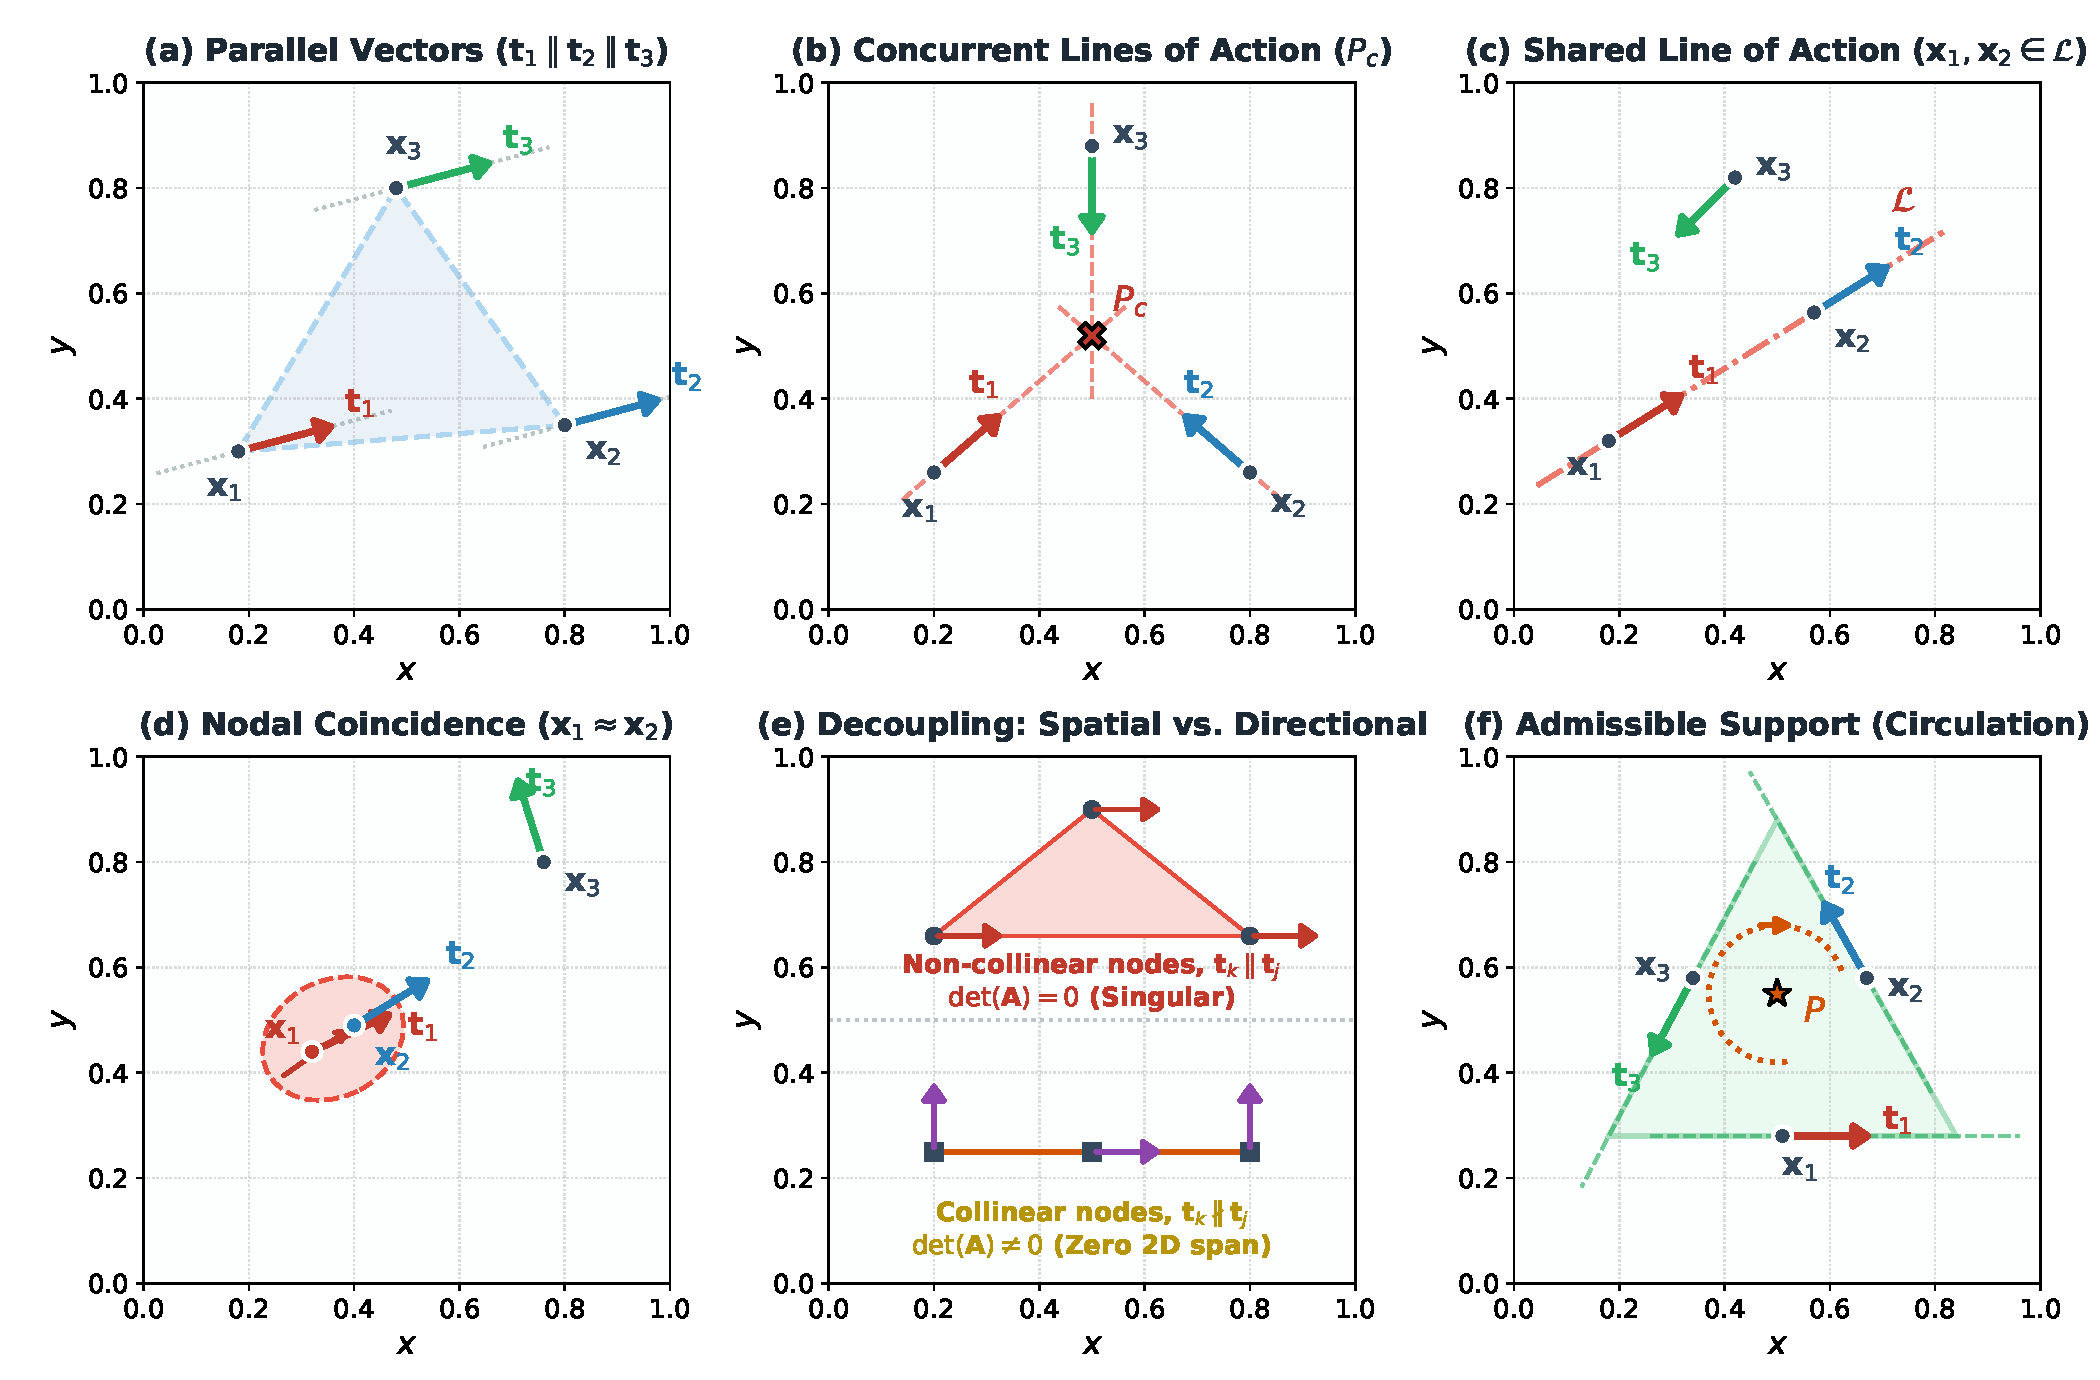
\includegraphics[width=\textwidth]{figura_singularidades_matriz_A.pdf}
\caption{Geometric and directional singularity configurations of the VNMM 2D local placement matrix $\mathbf{A} \in \mathbb{R}^{3 \times 3}$ for the $\mathcal{L}^1$ solenoidal vector basis:
(a) \textbf{Global vector parallelism} ($\vec{t}_1 \parallel \vec{t}_2 \parallel \vec{t}_3$): yields $t_{kx} = c\,t_{ky}$ for all $k$, causing linear dependency between the first two columns ($\operatorname{Col}_1(\mathbf{A}) = c\,\operatorname{Col}_2(\mathbf{A})$);
(b) \textbf{Concurrent lines of action}: when the lines of action of all three directors intersect at a common focal point $P_c(x_c, y_c)$, the relation $t_{kx}(y_k - y_c) - t_{ky}(x_k - x_c) = 0$ renders the rotational column a linear combination of the translation columns, yielding $\operatorname{Col}_3(\mathbf{A}) = y_c\operatorname{Col}_1(\mathbf{A}) - x_c\operatorname{Col}_2(\mathbf{A})$, causing $\det(\mathbf{A}) = 0$;
(c) \textbf{Shared line of action}: nodes $\mathbf{x}_1, \mathbf{x}_2$ lying on a common line $\mathcal{L}$ with $\vec{t}_1 = \vec{t}_2 \parallel (\mathbf{x}_2 - \mathbf{x}_1)$ share identical directional moments, $y_2 t_{2x} - x_2 t_{2y} = y_1 t_{1x} - x_1 t_{1y}$, producing duplicate rows $\operatorname{Row}_2(\mathbf{A}) = \operatorname{Row}_1(\mathbf{A})$;
(d) \textbf{Nodal coincidence / spatial collapse}: as $\|\mathbf{x}_1 - \mathbf{x}_2\| \to 0$, if $\vec{t}_1 = \vec{t}_2$ identical rows are formed; if $\vec{t}_1 \neq \vec{t}_2$, two distinct vector degrees of freedom are colocated at a single spatial point, degenerating the 2D spatial sampling base into a 1D line;
(e) \textbf{Decoupling of spatial geometry and vector alignment}: illustrates why geometric proximity algorithms alone fail---(top) spatially non-collinear nodes ($\operatorname{Area}(T) > 0$) with parallel directors yield $\det(\mathbf{A}) = 0$; (bottom) collinear nodes ($\operatorname{Area}(T) = 0$) with non-parallel directors can yield $\det(\mathbf{A}) \neq 0$ (algebraically invertible), yet fail to span 2D transverse derivatives;
(f) \textbf{Admissible and stable support}: dual qualification requiring non-collinear spatial distribution ($\operatorname{Area}(T) > 0$) and non-vanishing circulation around evaluation point $P$, ensuring $|\det(\mathbf{A})| \ge \mathrm{Tol}_{\det}(h)$ and promoting bounded condition numbers $\kappa(\mathbf{A}) \sim \mathcal{O}(1)$ for accurate field and curl reconstruction.}
\label{fig:vnmm_singularities_matrix_A}
\end{figure*}


% ---------------------------------------------------------
% SUBSECTION 3.1: L1 BASIS SINGULARITIES (3x3 MATRIX)
% ---------------------------------------------------------
\subsection{Singularities and Geometric Constraints in the Incomplete \texorpdfstring{$\mathcal{L}^1$}{L1} Basis (\texorpdfstring{$3 \times 3$}{3x3} Matrix)}
\label{subsec:singularities_L1}

To establish a systematic classification of algebraic singularities in the original VNMM 2D formulation \cite{ortiz2021nodal, ortiz2023tese}, we revisit the $3 \times 3$ local moment placement matrix $\mathbf{A}$ generated by the 3-node solenoidal basis $\mathcal{L}^1$. Originally derived in Eq.~\eqref{eq:matrix_A_L1}, $\mathbf{A}$ is restated below to facilitate the singularity analysis:
\begin{equation}
\mathbf{A} = \begin{bmatrix}
t_{1x} & t_{1y} & y_1 t_{1x} - x_1 t_{1y} \\[4pt]
t_{2x} & t_{2y} & y_2 t_{2x} - x_2 t_{2y} \\[4pt]
t_{3x} & t_{3y} & y_3 t_{3x} - x_3 t_{3y}
\end{bmatrix}
\label{eq:matrix_A_L1_revisited}
\end{equation}

For this matrix, algebraic singularity ($\det(\mathbf{A}) = 0$) occurs when the spatial-directional equations contributed by the candidate triad become linearly dependent \cite{ortiz2023tese, goncalves2025tese}. As classified visually in Figs.~\ref{fig:vnmm_singularities_matrix_A}a--\ref{fig:vnmm_singularities_matrix_A}d, these mathematical failures fall into four distinct pathological configurations:

\begin{enumerate}
    \item \textbf{Global Vector Parallelism (Fig.~\ref{fig:vnmm_singularities_matrix_A}a):} If all three unit directors are parallel or anti-parallel ($\vec{t}_1 \parallel \vec{t}_2 \parallel \vec{t}_3$), director components satisfy $t_{kx} = c \cdot t_{ky}$ for a constant scalar $c$. Thus, $\operatorname{Col}_1(\mathbf{A}) = c \cdot \operatorname{Col}_2(\mathbf{A})$, yielding $\det(\mathbf{A}) \equiv 0$ regardless of nodal spatial distribution.
    
    \item \textbf{Concurrency of Lines of Action (Fig.~\ref{fig:vnmm_singularities_matrix_A}b):} If the infinite lines of action passing through $\mathbf{x}_k$ along $\vec{t}_k$ intersect at a single common point $P_c(x_c, y_c)$, every node satisfies $t_{kx}(y_k - y_c) - t_{ky}(x_k - x_c) = 0$. This forces the rotational column $\operatorname{Col}_3$ to become a linear combination of translation columns, $\operatorname{Col}_3 = y_c \operatorname{Col}_1 - x_c \operatorname{Col}_2$, causing $\det(\mathbf{A}) = 0$.
    
    \item \textbf{Overlapping Lines of Action (Fig.~\ref{fig:vnmm_singularities_matrix_A}c):} If two support nodes lie on a common line $\mathcal{L}$ with directors aligned parallel to $\mathcal{L}$, the second row becomes identical to the first ($\operatorname{Row}_2 = \operatorname{Row}_1$), causing rank deficiency ($\operatorname{rank}(\mathbf{A}) \le 2$).
    
    \item \textbf{Nodal Coincidence / Spatial Collapse (Fig.~\ref{fig:vnmm_singularities_matrix_A}d):} Shared spatial coordinates ($\mathbf{x}_i \approx \mathbf{x}_j$) collapse spatial moment sampling, preventing 2D vector interpolation span.
\end{enumerate}

\subsubsection{Decoupling of Spatial Geometry and Vector Alignment}
\label{subsubsec:decoupling_L1}

A crucial theoretical insight governing vector meshless approximations is the formal decoupling between spatial sampling quality and vector algebraic independence, as explicitly highlighted in Fig.~\ref{fig:vnmm_singularities_matrix_A}e:

\begin{itemize}
    \item \textbf{Spatially Ideal but Algebraically Singular (Fig.~\ref{fig:vnmm_singularities_matrix_A}e, top):} A candidate triad can form an optimal 2D spatial distribution (e.g., an equilateral triangle enclosing a large physical area $|T| > 0$). A purely spatial geometric filter or distance-based $k$-d tree query would readily accept this support. However, if the assigned vector directors are globally parallel ($\vec{t}_1 \parallel \vec{t}_2 \parallel \vec{t}_3$), matrix $\mathbf{A}$ is strictly singular ($\det(\mathbf{A}) = 0$), rendering shape function construction impossible.
    
    \item \textbf{Algebraically Solvable but Spatially Degenerate (Fig.~\ref{fig:vnmm_singularities_matrix_A}e, bottom):} Conversely, if three support nodes lie on a perfectly collinear 1D line in space (zero triangle area $|T| = 0$) but possess non-parallel directors, matrix $\mathbf{A}$ in the $\mathcal{L}^1$ basis can yield a non-zero determinant ($\det(\mathbf{A}) \neq 0$). While algebraically solvable, this configuration lacks 2D spatial sampling normal to the line of nodes, leading to unconstrained polynomial extrapolation and catastrophic derivative errors in field operators.
    
\end{itemize}
In contrast to the pathological or decoupled configurations depicted in Figs.~\ref{fig:vnmm_singularities_matrix_A}(a)--(e), an admissible support---designated as an ideal support triad in Fig.~\ref{fig:vnmm_singularities_matrix_A}(f)---requires a dual geometric-directional qualification. Geometrically, the candidate support nodes must form a non-degenerate 2D spatial distribution ($|T| > 0$), shielding the local domain from nodal collapse or spatial collinearity. Directionally, the assigned vector directors $\vec{t}_k$ must provide coherent tangential circulation around the evaluation point $P(x_P, y_P)$, maximizing the directional moment $M_k = (\Delta\mathbf{x}_k \times \vec{t}_k)_z \gg 0$. By enforcing non-zero spatial area coverage and vector circulation simultaneously, the scale-dependent selection algorithm rejects locally degenerate configurations and enforces the criterion $|\det(\mathbf{A})| \ge \mathrm{Tol}_{\mathrm{det}}(h)$, thereby reducing the risk of ill-conditioned local placement matrices and promoting stable shape-function construction.

% ---------------------------------------------------------
% SUBSECTION 3.2: SINGULARITY ANALYSIS IN THE COMPLETE P1 BASIS (6x6 MATRIX)
% ---------------------------------------------------------
\subsection{Singularity Analysis in the Complete \texorpdfstring{$\mathcal{P}^1$}{P1} Vector Basis (\texorpdfstring{$6 \times 6$}{6x6} Matrix)}
\label{subsec:singularities_P1}

To eliminate derivative modal aliasing and achieve strict first-order convergence $\mathcal{O}(h^1)$ for the field curl operator $(\nabla \times \vec{E}^h)_z$, Section~\ref{subsec:complete_P1_basis} introduced the complete linear polynomial vector space $\mathcal{P}^1 = \mathcal{P}_1 \times \mathcal{P}_1$ ($M_{\mathrm{supp}} = 6$ support nodes). Imposing the vector Kronecker delta projection property across a candidate sextet yields a local placement system governed by the $6 \times 6$ local moment placement matrix $\mathbf{A} \in \mathbb{R}^{6 \times 6}$. Evaluated in local translated coordinates centered at the evaluation point $P(x_P, y_P)$ ($\Delta x_k = x_k - x_P, \Delta y_k = y_k - y_P$), matrix $\mathbf{A}$ was derived in Eq.~\eqref{eq:matrix_A_6x6} and is restated below to facilitate the singularity analysis:
\begin{equation}
\mathbf{A} = \begin{bmatrix}
t_{1x} & t_{1y} & \Delta x_1 t_{1x} & \Delta y_1 t_{1x} & \Delta x_1 t_{1y} & \Delta y_1 t_{1y} \\[4pt]
t_{2x} & t_{2y} & \Delta x_2 t_{2x} & \Delta y_2 t_{2x} & \Delta x_2 t_{2y} & \Delta y_2 t_{2y} \\[4pt]
t_{3x} & t_{3y} & \Delta x_3 t_{3x} & \Delta y_3 t_{3x} & \Delta x_3 t_{3y} & \Delta y_3 t_{3y} \\[4pt]
t_{4x} & t_{4y} & \Delta x_4 t_{4x} & \Delta y_4 t_{4x} & \Delta x_4 t_{4y} & \Delta y_4 t_{4y} \\[4pt]
t_{5x} & t_{5y} & \Delta x_5 t_{5x} & \Delta y_5 t_{5x} & \Delta x_5 t_{5y} & \Delta y_5 t_{5y} \\[4pt]
t_{6x} & t_{6y} & \Delta x_6 t_{6x} & \Delta y_6 t_{6x} & \Delta x_6 t_{6y} & \Delta y_6 t_{6y}
\end{bmatrix}
\label{eq:matrix_A_P1_repeated}
\end{equation}

By the Null-Space Orthogonality Principle, a non-zero coefficient vector $\mathbf{c} = [a_1, a_2, b_1, b_2, b_3, b_4]^T \in \mathbb{R}^6$ belongs to $\ker(\mathbf{A}_{6 \times 6})$ if and only if the corresponding affine vector field $\vec{E}(\mathbf{x}) \in \mathcal{P}^1$ (with components $E_x = a_1 + b_1 \Delta x + b_2 \Delta y$ and $E_y = a_2 + b_3 \Delta x + b_4 \Delta y$) satisfies the directional orthogonality condition $\vec{E}(\mathbf{x}_k) \cdot \vec{t}_k = 0$ across all six support nodes simultaneously. This characterizes exact singularity as the existence of a non-trivial affine vector field pointwise orthogonal to all six nodal directors.

In analyzing stencil stability, it is essential to distinguish clearly between three algebraic levels:
\begin{itemize}
    \item \textbf{Exact singularity ($\det(\mathbf{A}) = 0$):} Represents strict rank deficiency ($\operatorname{rank}(\mathbf{A}) < 6$) and a non-trivial null space ($\ker(\mathbf{A}) \neq \{\mathbf{0}\}$), where inversion is mathematically impossible;
    \item \textbf{Near-singularity ($|\det(\mathbf{A})| \ll 1$):} Occurs when candidate support sextets lie in the close algebraic vicinity of the singular hypersurface in configuration space; and
    \item \textbf{Poor conditioning ($\kappa_2(\mathbf{A}) \gg 1$):} Measured by the ratio of extremal singular values $\kappa_2(\mathbf{A}) = \sigma_{\max} / \sigma_{\min}$, quantifying the numerical error magnification under inversion.
\end{itemize}
Because $\det(\mathbf{A}) = \prod_{i=1}^6 \sigma_i$, the determinant governs the product of singular values rather than their ratio. A lower bound on $|\det(\mathbf{A})|$ therefore does not mathematically guarantee bounded conditioning in an arbitrary setting. However, under the localized spatial proximity constraints enforced during candidate support generation (where $\|\Delta \mathbf{x}_k\| \lesssim h$ naturally bounds $\sigma_{\max}$), bounding the product of singular values away from zero effectively impedes $\sigma_{\min} \to 0$.

While the complete $\mathcal{P}^1$ basis inherits the classical spatial-directional pathologies of $\mathcal{L}^1$ (such as global director parallelism and action-line concurrency), expanding the local placement space to 6 degrees of freedom creates new linear dependence modes. Specifically, algebraic analysis reveals four analytically identified singularity mechanisms governing $\mathbf{A}_{6 \times 6}$:

\begin{enumerate}
    \item \textbf{Partial Vector Parallelism (4-Node Threshold):} In contrast to $\mathcal{L}^1$ (which requires all 3 nodes to be parallel to collapse rank), $\mathbf{A}_{6 \times 6}$ becomes strictly singular ($\det(\mathbf{A}) \equiv 0$, $\operatorname{rank}(\mathbf{A}) \le 5$) whenever \textbf{4 or more nodes} in a candidate sextet possess parallel vector directors, with $\vec{t}_1 \parallel \vec{t}_2 \parallel \vec{t}_3 \parallel \vec{t}_4$. Under coordinate rotation aligning the common direction with $\hat{x}$ ($t_{ky} = 0$), columns 2, 5, and 6 contain zeros in the first 4 rows, confining 3 vector columns to a 2-dimensional active row space and forcing linear dependence regardless of nodal spatial locations or the remaining 2 directors.

    \item \textbf{Partial Spatial Collinearity (5-Node Threshold):} If \textbf{5 of the 6 support nodes} lie on a single straight line in 2D space ($\Delta y_k = m \Delta x_k$ for $k=1,\dots,5$), columns 4 ($\Delta y_k t_{kx}$) and 6 ($\Delta y_k t_{ky}$) possess non-zero entries exclusively in the 6th row ($\operatorname{Col}_4 \propto \operatorname{Col}_6$). This direct column proportionality forces $\det(\mathbf{A}_{6 \times 6}) = 0$, regardless of the vector directors assigned to all six nodes.

    \item \textbf{Total Spatial Collinearity Collapse (6 Nodes):} While 1D collinear nodes in $\mathcal{L}^1$ could yield a non-zero determinant if assigned non-parallel directors (becoming "algebraically solvable but spatially degenerate"), transitioning to $\mathcal{P}^1$ eliminates this spatial vulnerability. If all 6 support nodes are collinear in 2D space ($\Delta y_k = m \Delta x_k$), two independent column dependencies arise simultaneously ($\operatorname{Col}_4 = m \operatorname{Col}_3$ and $\operatorname{Col}_6 = m \operatorname{Col}_5$), collapsing the matrix rank to $\operatorname{rank}(\mathbf{A}) \le 4$, which implies $\det(\mathbf{A}_{6 \times 6}) \equiv 0$ unconditionally.

    \item \textbf{Azimuthal Divergence Masking ($\vec{t}_k \perp \Delta \mathbf{x}_k$):} While pure concentric circulation ($\vec{t}_k \perp \Delta \mathbf{x}_k$) represented the optimal configuration for $\mathcal{L}^1$, it induces strict singularity in $\mathcal{P}^1$. Enforcing pure azimuthal alignment sets $\Delta x_k t_{kx} + \Delta y_k t_{ky} = 0$, yielding $\operatorname{Col}_3 = -\operatorname{Col}_6$ and rendering $\det(\mathbf{A}_{6 \times 6}) = 0$. Physically, pure azimuthal directors cannot sample the linear isotropic divergence mode $\vec{E}_{\mathrm{div}} = [\Delta x, \Delta y]^T \in \mathcal{P}^1$, requiring the candidate support sextet to possess angular diversity containing both tangential and radial components.
\end{enumerate}


% ---------------------------------------------------------
% SECTION 3.3: AUTOMATED SUPPORT SELECTION ALGORITHM
% ---------------------------------------------------------
\subsection{Automated Support Selection Algorithm with Scale-Dependent Determinant Floor}
\label{sec:support_selection_algorithm}

The mathematical classifications established in Sections~\ref{subsec:singularities_L1} and \ref{subsec:singularities_P1} demonstrate that matrix singularity in the VNMM local placement system ($\mathbf{A} \boldsymbol{\beta}_i = \mathbf{L}_i$) stems from an intricate coupling between spatial node distributions $(\Delta x_k, \Delta y_k)$ and unit vector director alignments $(t_{kx}, t_{ky})$. Furthermore, as established by the Null-Space Orthogonality Principle, the set of singular configurations forms an algebraic hypersurface: whenever the nodal directors happen to be pointwise orthogonal to any non-trivial affine vector field $\vec{E} \in \mathcal{P}^1$ ($\vec{t}_k \propto R_{90} \vec{E}(\mathbf{x}_k)$), $\mathbf{A}_{6 \times 6}$ becomes strictly singular, even in generic non-collinear point distributions with non-parallel directors. Consequently, attempting to construct a purely heuristic geometric selection scheme---relying on explicit conditional decision trees to test for individual geometric pathologies---is not only impractically complex and fragile, but fundamentally incomplete.

In contrast, evaluating the magnitude of the determinant $|\det(\mathbf{A}_{6\times6})|$ of the local moment placement matrix serves as a unified algebraic filter against exact and near-singular configurations. Because $\mathbf{A}_{6\times6}$ incorporates both spatial coordinates and vector director projections within a single operator, enforcing $|\det(\mathbf{A}_{6\times6})| \ge \mathrm{Tol}_{\mathrm{det}}(h)$ simultaneously screens out exact singular configurations (such as spatial collapse, partial vector parallelism, action-line concurrency, divergence masking, and arbitrary null-space orthogonality alignments) as well as candidate sextets in their immediate near-singular vicinity.

% ---------------------------------------------------------
% SUBSECTION 3.3.1: SCALE-DEPENDENT SCALING LAW AND ABSOLUTE TOLERANCE FLOOR
% ---------------------------------------------------------
\subsubsection{Scale-Dependent Scaling Law, Dimensional Analysis, and Absolute Tolerance Floor}
\label{subsec:scale_dependent_floor}

In local translated coordinates centered at the evaluation point $P(x_P, y_P)$, the first two columns of $\mathbf{A} \in \mathbb{R}^{6 \times 6}$ consist of dimensionless unit director components $t_{kx}, t_{ky} \sim \mathcal{O}(1)$, while columns 3--6 contain products of coordinates and directors, $\Delta x_k t_{kx}, \Delta y_k t_{kx}, \Delta x_k t_{ky}, \Delta y_k t_{ky} \sim \mathcal{O}(h)$ [m], where $h$ denotes the local characteristic nodal spacing. Consequently, the local placement matrix is dimensional, and its determinant scales dimensionally as $[\det(\mathbf{A}_{6\times6})] = [L]^4$:
\begin{equation}
\det(\mathbf{A}_{6\times6}) \sim \mathcal{O}(h^4).
\label{eq:det_quartic_scaling}
\end{equation}
To interpret the determinant threshold independently of physical unit choices, one may consider the normalized, dimensionless local coordinates $\hat{x}_k = \Delta x_k / h$ and $\hat{y}_k = \Delta y_k / h$. The resulting dimensionless placement matrix $\widehat{\mathbf{A}}$ satisfies $\mathbf{A} = \widehat{\mathbf{A}} \, \operatorname{diag}(1, 1, h, h, h, h)$, directly establishing:
\begin{equation}
\det(\mathbf{A}) = h^4 \det(\widehat{\mathbf{A}}).
\label{eq:dimensionless_det_relation}
\end{equation}
Thus, a scale-invariant algebraic qualification criterion is equivalent to bounding the dimensionless determinant $|\det(\widehat{\mathbf{A}})| \ge \widehat{\mathrm{Tol}} > 0$.

Under spatial refinement ($h \to 0$), enforcing a purely proportional scaling law based on a fixed reference grid ($h_{\mathrm{ref}}$):
\begin{equation}
\mathrm{Tol}_{\mathrm{det}}^{\mathrm{pure}}(h) = \mathrm{Tol}_{\mathrm{ref}} \cdot \left( \frac{h}{h_{\mathrm{ref}}} \right)^4
\label{eq:pure_quartic_law}
\end{equation}
produces an excessively permissive threshold in dense point clouds (e.g., $\mathrm{Tol}_{\mathrm{det}} \approx 1.2 \times 10^{-6}$ for $h = 0.0654$\,m over $[0, \pi]^2$). As demonstrated through the parametric numerical experiments in Section~\ref{subsubsec:quartic_law_failure}, such unconstrained low thresholds cause the early-stopping selection mechanism to prematurely accept candidate sextets exhibiting poor angular diversity. In terms of the dimensionless matrix, this allows $|\det(\widehat{\mathbf{A}})|$ to approach zero, which elevates the condition number $\kappa_2(\mathbf{A}) > 170$ and induces local derivative degradation and stagnation in the curl approximation.

To establish an effective algebraic rejection criterion against near-degenerate supports across all spatial discretization scales, the proposed framework enforces a scale-dependent determinant thresholding law with an absolute tolerance floor $\mathrm{Tol}_{\mathrm{floor}}$:
\begin{equation}
\mathrm{Tol}_{\mathrm{det}}(h) = \max \left( \mathrm{Tol}_{\mathrm{ref}} \cdot \left( \frac{h}{h_{\mathrm{ref}}} \right)^4, \; \mathrm{Tol}_{\mathrm{floor}} \right).
\label{eq:scale_dependent_determinant_floor}
\end{equation}

While a determinant lower bound controls the product of singular values ($\prod_{i=1}^6 \sigma_i$) rather than their ratio directly ($\kappa_2(\mathbf{A}) = \sigma_{\max} / \sigma_{\min}$), the determinant criterion was found empirically to provide an effective support-rejection surrogate for poor conditioning under the tested spatial-proximity constraints. In the investigated benchmark configurations, this algebraic rejection criterion maintained $\kappa_2(\mathbf{A}) \le 73$ at the baseline floor $\mathrm{Tol}_{\mathrm{floor}} = 1.5 \times 10^{-5}$ and reached $\approx 64$ at a compromise threshold of $3.0 \times 10^{-5}$ that balances conditioning, curl error, and compact neighborhood size. By setting $\mathrm{Tol}_{\mathrm{floor}} = 1.5 \times 10^{-5}$ for the domain $\Omega = [0, \pi]^2$, the selection pipeline is forced to dynamically expand its candidate neighborhood search whenever spatial or directional alignment degrades in dense or perturbed clouds. Dimensionally, on a general domain with characteristic dimension $L_{\mathrm{domain}}$, the floor scales as $\mathrm{Tol}_{\mathrm{floor}} \propto (L_{\mathrm{domain}})^4 \widehat{\mathrm{Tol}}_{\mathrm{floor}}$. However, because $\mathrm{Tol}_{\mathrm{floor}} = 1.5 \times 10^{-5}$ is an empirically calibrated parameter for the tested $[0, \pi]^2$ domain, establishing whether this scaling law yields a universally transferable threshold across arbitrary geometries, non-uniform nodal density gradients, or anisotropic director distributions remains an open question. As quantitatively validated in Section~\ref{subsubsec:restoration_via_floor}, this floor enables the identification of an admissible support under the tested thresholding strategy, yielding stable local configurations and restoring monotonic error reduction in the tested refinement sequences without a significant increase in computational cost.

\subsubsection{The 4-Phase Selection Pipeline}
\label{subsec:4phase_pipeline}

To locate well-conditioned candidate sextets across unstructured point clouds without incurring exhaustive $\mathcal{O}(N^2)$ pairwise distance evaluations, the proposed selection framework combines orthogonal $k$-d tree spatial queries \cite{bentley1975multidimensional,parreira2006efficient,fasshauer2007meshfree,goncalves2025tese} with algebraic determinant qualification. The resulting algorithm operates through a 4-phase pipeline:

\begin{enumerate}
    \item \textbf{Phase 1: Spatial Neighborhood Query via $k$-d Tree:} Using an orthogonal $k$-d tree binary spatial search structure constructed over all domain nodes ($\mathcal{O}(N \log N)$ pre-processing complexity), the algorithm queries the $K_{\mathrm{initial}} \ge 12$ nearest physical neighbors surrounding the evaluation point $P(x_P, y_P)$ with an average query complexity of $\mathcal{O}(\log N)$ \cite{bentley1975multidimensional, parreira2006efficient, fasshauer2007meshfree}.
    
    \item \textbf{Phase 2: Combinatorial Candidate Generation with Progressive Anchor:} Candidate support sextets are generated systematically from the queried $K_{\mathrm{initial}}$ neighborhood. To prioritize geometric proximity to the evaluation point $P$, candidate sextets are assembled by fixing an anchor node (beginning with the node closest to $P$) and taking 5-combinations from subsequent nearest neighbors, ordered by increasing mean Euclidean distance.
    
    \item \textbf{Phase 3: Local Coordinate Translation and Matrix Assembly:} For each candidate sextet, spatial coordinates are translated to the local evaluation frame ($\Delta x_k = x_k - x_P, \Delta y_k = y_k - y_P$), and the local placement matrix $\mathbf{A}_{6 \times 6}$ is assembled using Eq.~\eqref{eq:matrix_A_P1_repeated}.
    
    \item \textbf{Phase 4: Algebraic Qualification with Early Stopping:} The determinant magnitude $|\det(\mathbf{A}_{6\times6})|$ is computed. The first candidate sextet satisfying the scale-dependent criterion $|\det(\mathbf{A}_{6\times6})| \ge \mathrm{Tol}_{\mathrm{det}}(h)$ via Eq.~\eqref{eq:scale_dependent_determinant_floor} is immediately accepted as the active support, terminating the local search loop.
\end{enumerate}

\subsubsection{Computational Complexity and Combinatorial Cost Analysis}
\label{subsubsec:computational_complexity}

A critical aspect of practical meshless implementations concerns the algorithmic complexity of support selection \cite{slak2018refined}. In analyzing this pipeline, it is essential to distinguish clearly among three separate concepts: (i) the asymptotic complexity of the spatial neighborhood search, (ii) the theoretical worst-case combinatorial bound of candidate support generation, and (iii) the observed empirical cost achieved through early stopping.

The $k$-d tree provides logarithmic average neighborhood-query cost under standard assumptions ($\mathcal{O}(\log N)$ per evaluation point, preceded by an $\mathcal{O}(N \log N)$ one-off tree construction cost) \cite{bentley1975multidimensional, parreira2006efficient, fasshauer2007meshfree}, whereas the subsequent support qualification has a worst-case combinatorial cost bounded by the binomial coefficient:
\begin{equation}
N_{\mathrm{comb}}^{\mathrm{max}} = \binom{K_{\mathrm{initial}}}{6}.
\label{eq:binomial_combinations}
\end{equation}
For the baseline initial neighborhood of $K_{\mathrm{initial}} = 12$ nodes employed in this work, Eq.~\eqref{eq:binomial_combinations} yields $\binom{12}{6} = 924$ potential candidate sextets. If an exhaustive search were conducted across all candidate combinations, the algebraic qualification cost per evaluation point would scale as $C_{\mathrm{eval}}^{\mathrm{exhaustive}} \approx \binom{K_{\mathrm{initial}}}{6} C_{\det}$, where $C_{\det} \sim \mathcal{O}(6^3) = \mathcal{O}(1)$ denotes the fixed floating-point cost of evaluating a $6 \times 6$ determinant. While $\binom{K_{\mathrm{initial}}}{6}$ represents a local upper bound that is asymptotically independent of the global node count $N$, evaluating all combinations would still represent a substantial computational overhead across $N_{\mathrm{eval}}$ evaluation points.

Crucially, however, the proposed selection algorithm does \emph{not} perform an exhaustive sweep. By coupling progressive proximity-ordered candidate generation (Phase~2) with the \textbf{early-stopping qualification criterion} (Phase~4), the search evaluates candidate sextets sequentially and terminates immediately once an admissible support satisfying $|\det(\mathbf{A}_{6 \times 6})| \ge \mathrm{Tol}_{\mathrm{det}}(h)$ is identified. 

This establishes a necessary distinction between the \emph{neighborhood query size} ($K_{\mathrm{avg}}$, the physical number of nearest neighbors retrieved from the $k$-d tree) and the \emph{qualification count} ($\bar{N}_{\mathrm{tested}}$, the actual number of candidate sextets evaluated algebraically via $\det(\mathbf{A}_{6\times6})$ before an admissible support is found). While a retrieved neighborhood of $K \approx 11$ nodes contains $\binom{11}{6} = 462$ potential candidate sextets, in the present implementation, however, early stopping reduces the observed number of determinant evaluations to $2.61\text{--}4.64$ per evaluation point for the tested cavity sequence.

To establish the computational efficiency of early stopping, Table~\ref{tab:support_selection_cost} reports the empirical performance metrics measured across six refinement levels of the electromagnetic resonant cavity problem (formally formulated in Section~\ref{sec:variational_formulation} and investigated in Section~\ref{subsec:convergence_comparison}), evaluated at $N_{\mathrm{eval}} = 400$ Gauss integration points.

\begin{table}[!htbp]
\centering
\caption{Computational cost of automated support selection across six cavity discretization levels ($N_{\mathrm{eval}} = 400$ Gauss evaluation points, $K_{\mathrm{initial}} = 12$).}
\label{tab:support_selection_cost}
\resizebox{\columnwidth}{!}{%
\begin{tabular}{@{} c c c c c c @{}}
\toprule
\textbf{Grid Nodes} & \textbf{Mean Neighbors} & \multicolumn{2}{c}{\textbf{Evaluated Sextets ($N_{\mathrm{tested}}$)}} & \textbf{Support Time} & \textbf{Assembly Time} \\
\cmidrule(lr){3-4}
$N$ & $K_{\mathrm{avg}}$ & \textbf{Mean} ($\bar{N}_{\mathrm{tested}}$) & \textbf{Maximum} & $t_{\mathrm{sup}}$ [s] & $t_{\mathrm{ass}}$ [s] \\
\midrule
$81$ ($9 \times 9$)     & 6.6 & $\mathbf{3.75}$ & 29 & 0.012 & 0.025 \\
$169$ ($13 \times 13$)  & 6.6 & $\mathbf{3.88}$ & 29 & 0.012 & 0.025 \\
$289$ ($17 \times 17$)  & 6.6 & $\mathbf{4.64}$ & 29 & 0.014 & 0.027 \\
$441$ ($21 \times 21$)  & 7.1 & $\mathbf{3.21}$ &  9 & 0.011 & 0.023 \\
$625$ ($25 \times 25$)  & 6.7 & $\mathbf{2.61}$ &  8 & 0.009 & 0.023 \\
$841$ ($29 \times 29$)  & 6.6 & $\mathbf{2.77}$ &  8 & 0.010 & 0.022 \\
\bottomrule
\end{tabular}%
}
\end{table}

As shown in Table~\ref{tab:support_selection_cost}, the actual number of candidate sextets evaluated per evaluation point remains remarkably small: $\bar{N}_{\mathrm{tested}}$ ranges from $2.61$ to $4.64$ sextets, with the maximum evaluations never exceeding $29$ across all $400$ quadrature points. Support qualification consumes only $0.009\text{--}0.014$\,s, representing approximately $40\%$ of the total global matrix assembly time ($t_{\mathrm{ass}} \approx 0.025$\,s). 

Even under $25\%$ stochastic spatial jitter and random director orientations (Section~\ref{subsec:stochastic_perturbations}), early stopping remains highly efficient: $\bar{N}_{\mathrm{tested}}$ averages $1.1\text{--}2.5$ sextets for $N \le 1{,}928$, rising to $\bar{N}_{\mathrm{tested}} \approx 40.7$ (with a peak of $293$ evaluations) only in the ultra-dense perturbed cloud ($N = 4{,}192$), where the absolute floor $\mathrm{Tol}_{\mathrm{floor}}$ forces wider combinatorial sampling to bypass near-parallel directors. Even in that extreme case, total support selection time for $400$ evaluation points is merely $0.10$\,s.

Distinguishing the worst-case bound ($\binom{K_{\mathrm{initial}}}{6} C_{\det}$) from the observed empirical cost, the total operational runtime across $N_{\mathrm{eval}}$ evaluation points can be expressed as:
\begin{align}
T_{\mathrm{support}} &= \underbrace{\mathcal{O}(N \log N)}_{\text{$k$-d tree construction}} \nonumber \\
&\quad + \sum_{p=1}^{N_{\mathrm{eval}}} \left[ \underbrace{\mathcal{O}(\log N)}_{\text{spatial query}} + \underbrace{\bar{N}_{\mathrm{tested}}^{(p)} \, C_{\det(6 \times 6)}}_{\text{observed algebraic qualification}} \right].
\label{eq:support_total_complexity}
\end{align}
While the worst-case qualification cost is bounded by $\binom{K_{\mathrm{initial}}}{6}$, the empirical early-stopping count remains very small ($\bar{N}_{\mathrm{tested}} \approx 2.6\text{--}4.6$ in unperturbed domains and moderate in perturbed clouds). Consequently, in the tested configurations, the observed support selection overhead is dominated by the logarithmic spatial neighbor query rather than by combinatorial matrix evaluations, reconciling robust support identification with practical computational efficiency.


% --- SEÇÃO 4: FORMULAÇÃO DA CAVIDADE ---
% =========================================================
% SECTION 4: VARIATIONAL FORMULATION OF THE RESONANT CAVITY PROBLEM
% =========================================================
\section{Variational Formulation of the Resonant Cavity Problem}
\label{sec:variational_formulation}

To evaluate the spectral accuracy and verify the suppression of non-physical spurious modes within the operational bandwidth in the Vector Nodal Meshless Method (VNMM 2D), we formulate the electromagnetic vector eigenvalue problem in a two-dimensional resonant cavity $\Omega = [0, \pi] \times [0, \pi] \subset \mathbb{R}^2$ with perfect electric conductor (PEC) walls $\partial\Omega$ \cite{harrington2001time}.

\subsection{The Transverse Electric (\texorpdfstring{$TE_z$}{TEz}) Vector Eigenvalue Problem}
\label{subsec:strong_form}

In a homogeneous, isotropic, and lossless dielectric medium ($\epsilon_r = 1.0, \mu_r = 1.0$), time-harmonic Transverse Electric modes ($TE_z$) are governed by the vector double-curl Helmholtz equation for the transverse electric field $\vec{E}(\mathbf{x}) = [E_x(x,y), E_y(x,y)]^T$ \cite{monk2003finite, ortiz2023tese}:
\begin{align}
\nabla \times \left( \frac{1}{\mu_r} \nabla \times \vec{E} \right) &= \lambda \, \epsilon_r \vec{E}, \quad \text{in } \Omega \label{eq:helmholtz_strong} \\
\hat{n} \times \vec{E} &= \mathbf{0}, \quad \text{on } \partial\Omega \label{eq:pec_boundary}
\end{align}
where $\lambda = k_0^2 = \omega^2 \mu_0 \epsilon_0$ denotes the target wavenumber eigenvalue, $\omega$ is the angular resonance frequency, and $\hat{n}$ is the outward unit normal vector to boundary $\partial\Omega$. In two dimensions, the curl operator acting on a 2D vector field yields a scalar normal component $(\nabla \times \vec{E})_z = \partial E_y/\partial x - \partial E_x/\partial y$, while the vector curl of a scalar field $u_z$ returns a vector in the transverse plane $\nabla \times u_z = [\partial u_z/\partial y, -\partial u_z/\partial x]^T$.

The exact analytical eigenvalues for the square PEC cavity are given by \cite{harrington2001time}:
\begin{equation}
\lambda_{m,n}^{\mathrm{exact}} = m^2 + n^2, \quad m,n \in \{0, 1, 2, \dots\}, \quad (m+n > 0)
\label{eq:analytical_eigenvalues}
\end{equation}

% ---------------------------------------------------------
% SUBSECTION 4.2: RITZ-GALERKIN WEAK FORM WITH DIV-CURL REGULARIZATION
% ---------------------------------------------------------
\subsection{Ritz-Galerkin Weak Form with Div-Curl Regularization}
\label{subsec:weak_form_regularization}
Let the Hilbert space of square-integrable vector fields with square-integrable curl satisfying homogeneous tangential PEC boundary conditions be defined as \cite{monk2003finite, bossavit1998computational}:
\begin{equation}
\mathcal{S} \triangleq \left\{ \vec{E} \in H(\mathrm{curl}; \Omega) \;\middle|\; \hat{n} \times \vec{E} = \mathbf{0} \text{ on } \partial\Omega \right\}.
\label{eq:hilbert_space_S}
\end{equation}
In standard Edge Finite Element Formulations (EFEM), the discrete space is globally $H(\mathrm{curl})$-conforming ($V_h \subset \mathcal{S}$) because shared tangential degrees of freedom across conforming element facets guarantee exact tangential trace continuity ($\hat{n} \times [\vec{E}^h] = \mathbf{0}$) \cite{monk2003finite, bossavit1990spurious}. Under this global conformity, the discrete de Rham complex property $\operatorname{Im}(\nabla) \subset \ker(\nabla \times)$ holds exactly: irrotational gradient fields ($\vec{E} = \nabla \phi$) yield an identically zero curl ($\nabla \times (\nabla \phi) \equiv \mathbf{0}$) and map directly into the zero eigenvalue subspace ($\lambda = 0$), preventing spectrum contamination without auxiliary constraints \cite{monk2003finite, boffi1999computational}.

In contrast, on arbitrary point clouds, the assembled meshless VNMM vector approximation is globally non-conforming ($V_h \not\subset \mathcal{S}$). Although each local vector shape function $\vec{N}_i(\mathbf{x})$ possesses local $H(\mathrm{curl})$ regularity within its local support stencil, the active support changes across the domain, producing minor tangential trace discontinuities across support boundaries. Consequently, the discrete de Rham complex does not hold exactly at background quadrature points, and discrete gradient states produce non-zero numerical curl residues ($\nabla \times (\nabla \phi) \neq \mathbf{0}$). This discrete gradient nullspace leakage causes spurious non-physical modes to infiltrate the low-frequency spectrum. To suppress these spurious modes without introducing saddle-point system indefiniteness or auxiliary Lagrange multipliers, we adopt a \textbf{Ritz-Galerkin weak formulation with div-curl penalty regularization} \cite{monk2003finite, bossavit1998computational}:
\begin{multline}
\int_{\Omega} \frac{1}{\mu_r} (\nabla \times \vec{W})_z (\nabla \times \vec{E})_z \, d\Omega + s_{\mathrm{div}} \int_{\Omega} (\nabla \cdot \vec{W}) (\nabla \cdot \vec{E}) \, d\Omega \\
= \lambda \int_{\Omega} \epsilon_r \vec{W} \cdot \vec{E} \, d\Omega, \quad \forall \vec{W} \in \mathcal{S}
\label{eq:regularized_weak_form}
\end{multline}
where $s_{\mathrm{div}} > 0$ is the non-dimensional divergence penalty parameter \cite{monk2003finite}.

Upon discretizing the electric field as $\vec{E}^h(\mathbf{x}) = \sum_{j=1}^{M} c_j \vec{N}_j(\mathbf{x})$ and test functions as $\vec{W}^h(\mathbf{x}) = \sum_{i=1}^{M} d_i \vec{N}_i(\mathbf{x})$, the second bilinear term in Eq.~\eqref{eq:regularized_weak_form} defines the \textbf{divergence penalty matrix} $\mathbf{K}_{\mathrm{div}} \in \mathbb{R}^{M \times M}$, whose entries $K_{\mathrm{div}, ij}$ are explicitly defined by:
\begin{equation}
K_{\mathrm{div}, ij} \triangleq \int_{\Omega} (\nabla \cdot \vec{N}_i) (\nabla \cdot \vec{N}_j) \, d\Omega
\label{eq:K_div_definition}
\end{equation}

Consequently, the global stiffness matrix $\mathbf{K}$ in the discrete generalized eigenvalue problem $\mathbf{K} \mathbf{c} = \lambda \mathbf{M} \mathbf{c}$ decomposes into the sum of the primary curl-curl stiffness matrix $\mathbf{K}_{\mathrm{curl}}$ and the scaled divergence penalty matrix $s_{\mathrm{div}} \mathbf{K}_{\mathrm{div}}$:
\begin{equation}
\mathbf{K} = \mathbf{K}_{\mathrm{curl}} + s_{\mathrm{div}} \mathbf{K}_{\mathrm{div}}
\label{eq:K_global_decomposition}
\end{equation}
with individual entries of the primary curl-curl stiffness matrix defined by:
\begin{equation}
K_{\mathrm{curl}, ij} \triangleq \int_{\Omega} \frac{1}{\mu_r} (\nabla \times \vec{N}_i)_z (\nabla \times \vec{N}_j)_z \, d\Omega.
\label{eq:K_curl_definition}
\end{equation}

The physical and algebraic role of the penalty matrix $\mathbf{K}_{\mathrm{div}}$ scaled by $s_{\mathrm{div}}$ is twofold \cite{monk2003finite, bossavit1990spurious}:
\begin{enumerate}
    \item \textbf{Asymptotic Preservation of Physical Modes:} Solenoidal physical $TE_z$ modes satisfy $\nabla \cdot \vec{E} \equiv 0$ analytically. At the continuous level, the divergence penalty term vanishes identically ($\int_\Omega (\nabla \cdot \vec{E})^2 d\Omega = 0$), leaving analytical physical eigenvalues unperturbed \cite{monk2003finite, jin2014finite}. In the discrete meshless formulation, because pointwise divergence is satisfied only approximately ($\nabla \cdot \vec{E}^h \sim \mathcal{O}(h)$), the penalty introduces a minor discrete perturbation that systematically decays under spatial refinement, maintaining the divergence-to-curl energy ratio $R_{\mathrm{div}} \triangleq \frac{\mathbf{c}^T \mathbf{K}_{\mathrm{div}} \mathbf{c}}{\mathbf{c}^T \mathbf{K}_{\mathrm{curl}} \mathbf{c}} \ll 1$ for physical modes.
    \item \textbf{Penalization of Gradient Modes:} Non-physical gradient fields satisfy $\nabla \cdot (\nabla \phi) = \Delta \phi \neq 0$. The penalty term $s_{\mathrm{div}} \mathbf{K}_{\mathrm{div}} \mathbf{c}$ adds artificial numerical stiffness to these states, shifting their spurious eigenvalues to high frequencies outside the operational bandwidth ($\lambda > 50$ in the tested cavity discretization) \cite{monk2003finite, bossavit1990spurious, boffi1999computational}.
\end{enumerate}
As demonstrated by the systematic parametric tuning in Section~\ref{subsec:cavity_eigenvalues}, the value $s_{\mathrm{div}} = 6.0$ was selected as a representative value within the tested stable penalty range ($s_{\mathrm{div}} \in [4.0, 10.0]$), achieving reliable spectral purification without inducing numerical locking.



\subsection{Integration Strategy: Cell-Based vs. Point-Based (EFG-Style)}
\label{subsec:integration_strategy}

Numerical evaluation of weak form integrals in Eq.~\eqref{eq:regularized_weak_form} requires background cell quadrature. In early VNMM implementations, support nodes and local moment placement matrices $\mathbf{A}$ were constructed once per background cell at its centroid $P_c$ \cite{ortiz2021nodal, ortiz2023tese}. However, as demonstrated by the background cell integration analysis in Section~\ref{sec:numerical_results}, expanding shape functions from $P_c$ across large cells ($dx > h$) induces severe Taylor truncation degradation and matrix indefiniteness.


To obtain a mesh-connectivity-free field approximation, we employ a point-based Element-Free Galerkin (EFG) integration strategy over a background integration grid \cite{belytschko1994element, parreira2006efficient}:
\begin{enumerate}
    \item A regular background grid of $N_c \times N_c$ quadrilateral integration cells (with $N_c = \operatorname{round}(0.6 N)$) covers the physical domain $\Omega$.
    \item At each Gauss integration point $P_g(x_g, y_g)$, the algorithm queries the global $k$-d tree independently to select an admissible, well-conditioned support sextet $\{P_k, \vec{t}_k\}_{k=1}^6$ satisfying $|\det(\mathbf{A}_{6 \times 6})| \ge \operatorname{Tol}_{\mathrm{det}}(h)$.
    \item Local translated coordinates are anchored directly at the evaluation point ($\Delta x = x_k - x_g = 0$, $\Delta y = y_k - y_g = 0$), ensuring that shape functions $\vec{N}_i(P_g)$ and their derivatives $\nabla \times \vec{N}_i(P_g)$, $\nabla \cdot \vec{N}_i(P_g)$ are evaluated with maximum floating-point precision without Taylor expansion drift.
\end{enumerate}
Employing a baseline $2 \times 2$ Gauss-Legendre quadrature rule (4 points per cell, providing $N_g / N_{\mathrm{DoF}} \approx 1.11$ in the baseline benchmark) balances integration fidelity and assembly speed, with higher-order rules ($3 \times 3$ and $4 \times 4$) evaluated parametrically in Section~\ref{subsubsec:quadrature_sensitivity}.

\paragraph{Classification as a Meshless Formulation}
In classical meshfree literature \cite{belytschko1994element, atluri2002meshless, liu2009mesh}, a distinction is drawn between methods that construct approximations free of mesh connectivity (such as EFG, PIM, and the present VNMM) and methods that evaluate weak integrals without background cells (such as nodal integration or MLPG). In the present VNMM formulation:
\begin{itemize}
    \item The field approximation and shape functions $\vec{N}_i(\mathbf{x})$ are strictly meshless and connectivity-free: no triangulation, polygonization, or element topological data structures are created or maintained between approximation nodes.
    \item Background quadrilateral cells serve solely as a geometric scaffolding for evaluating numerical integrals via Gauss-Legendre quadrature, exactly as in standard Element-Free Galerkin (EFG) schemes \cite{belytschko1994element, parreira2006efficient}.
    \item The background integration grid does not define or constrain the interpolation topology; support selection at any point is governed exclusively by $k$-d tree spatial proximity and algebraic determinant qualification.
\end{itemize}

\subsection{Algebraic Discretization and Generalized Eigenvalue System}
\label{subsec:algebraic_system}

Approximating the electric field as $\vec{E}^h(\mathbf{x}) = \sum_{i=1}^{M_{\mathrm{active}}} \vec{N}_i(\mathbf{x}) c_i$ and test functions as $\vec{W}^h(\mathbf{x}) = \sum_{j=1}^{M_{\mathrm{active}}} \vec{N}_j(\mathbf{x}) d_j$, where $c_i = \vec{E}(\mathbf{x}_i) \cdot \vec{t}_i$ represent the active directional projection DoFs, yields the sparse generalized algebraic eigenvalue system \cite{ortiz2023tese, goncalves2025tese}:
\begin{equation}
\mathbf{K}_{\mathrm{red}} \mathbf{c}_{\mathrm{red}} = \lambda \mathbf{M}_{\mathrm{red}} \mathbf{c}_{\mathrm{red}}
\label{eq:generalized_eigenvalue_system}
\end{equation}

The entries of the global stiffness matrix $\mathbf{K} \in \mathbb{R}^{M \times M}$ and mass matrix $\mathbf{M} \in \mathbb{R}^{M \times M}$ are assembled as \cite{goncalves2025tese}:
\begin{align}
K_{ij} &= \int_{\Omega} \frac{1}{\mu_r} (\nabla \times \vec{N}_i)_z (\nabla \times \vec{N}_j)_z \, d\Omega + s_{\mathrm{div}} \int_{\Omega} (\nabla \cdot \vec{N}_i)(\nabla \cdot \vec{N}_j) \, d\Omega \label{eq:stiffness_matrix_entry} \\
M_{ij} &= \int_{\Omega} \epsilon_r \, \vec{N}_i \cdot \vec{N}_j \, d\Omega \label{eq:mass_matrix_entry}
\end{align}

Homogeneous PEC boundary conditions ($\hat{n} \times \vec{E} = \mathbf{0}$) are enforced directly by setting $c_k = 0$ for all boundary nodes whose unit directors $\vec{t}_k$ align tangent to $\partial\Omega$ ($\vec{t}_k \parallel \partial\Omega$), reducing the system size to $M_{\mathrm{red}}$ active internal degrees of freedom (equivalently designated as $N_{\mathrm{DoF}} \equiv M_{\mathrm{red}}$ in subsequent convergence comparisons) \cite{ortiz2021nodal, goncalves2025tese}. While the unregularized Maxwell stiffness operator is symmetric positive-semidefinite due to the static gradient nullspace, the inclusion of the divergence penalty ($s_{\mathrm{div}} > 0$) combined with essential PEC boundary constraints renders $\mathbf{K}_{\mathrm{red}}$ strictly positive-definite on the discrete physical subspace, while the mass matrix $\mathbf{M}_{\mathrm{red}}$ is natively positive-definite. This ensures that the discrete generalized eigenvalue problem involves well-behaved, sparse symmetric positive-definite (SPD) reduced matrices, allowing efficient and stable computation of the physical spectrum using Krylov-subspace shift-and-invert Arnoldi methods \cite{saad2011numerical, lehoucq1998arpack}, as implemented via the ARPACK solver in SciPy \cite{virtanen2020scipy}.

% =========================================================
% SECTION 5: NUMERICAL RESULTS AND DISCUSSION
% =========================================================
\section{Numerical Verification and Validation}
\label{sec:numerical_results}

This section assesses the numerical performance of the proposed Vector Nodal Meshless Method (VNMM 2D). Following established guidelines in computational mechanics and electromagnetics, the numerical campaign is systematically organized into three complementary stages:
\begin{enumerate}
    \item \textbf{Numerical Verification (Sections~\ref{subsec:conforming_dual_equivalence}--\ref{subsec:stochastic_perturbations}):} Focused on the mathematical properties of the discretized operators, including exact dual isomorphism against Whitney 1-form finite elements on a single simplex, restoration of asymptotic curl convergence via the complete linear vector basis $\mathcal{P}^1$, and local algebraic placement matrix conditioning under stochastic spatial-directional jitter.
    \item \textbf{Physics-Based Spectral Validation (Sections~\ref{subsec:cavity_eigenvalues}--\ref{subsec:convergence_comparison}):} Focused on practical electromagnetic boundary-value problems, including Transverse Electric ($TE_z$) resonant cavity eigenvalue spectra under div-curl Ritz-Galerkin penalty regularization, and asymptotic convergence benchmarking against canonical Edge FEM across six mesh refinement levels.
    \item \textbf{Limitations and Scope of Applicability (Section~\ref{subsec:limitations_scope}):} Focused on establishing honest methodological boundaries, discussing background quadrature dependencies, extreme point-cloud anisotropy, penalty parameter sensitivity, and high-frequency dispersion.
\end{enumerate}

\subsection{Conforming Local Dual Equivalence: VNMM \texorpdfstring{$\mathcal{L}^1$}{L1} vs. Whitney EFEM}
\label{subsec:conforming_dual_equivalence}

To establish a rigorous baseline connecting the proposed vector meshless formulation to established finite element theory, this first experiment evaluates the local vector interpolation capacity of the incomplete 3-node basis $\mathcal{L}^1$ against lowest-order Whitney 1-form edge elements (N\'ed\'elec 1st-kind) \cite{nedelec1980mixed, monk2003finite}.

\subsubsection{Experimental Setup and Dual Topologies}
The benchmark test considers the $TE_{11}$ resonant mode over the square cavity domain $\Omega = [0, \pi] \times [0, \pi]$, governed by the exact analytical field \cite{harrington2001time, jin2014finite}:
\begin{equation}
\vec{E}_{\mathrm{ex}}(x, y) = \begin{bmatrix} \cos(x) \sin(y) \\[2pt] -\sin(x) \cos(y) \end{bmatrix}, \qquad (\nabla \times \vec{E}_{\mathrm{ex}})_z(x, y) = -2 \cos(x) \cos(y)
\label{eq:analytical_te11_field}
\end{equation}

To compare both formulations under identical spatial sampling, a sequence of seven conforming triangular meshes ($4\times4$ to $32\times32$) is generated with controlled stochastic vertex perturbation ($10\%$ jitter) to ensure arbitrary, non-equilateral simplices. All interpolation errors are evaluated across a fixed, invariant grid of $1{,}600$ internal Cartesian points ($40 \times 40$).

The geometric arrangement of the conforming dual topology is illustrated in Fig.~\ref{fig:malha_conforme_vnmm_L1}. For a triangular cell $T$ with vertices $V_1, V_2, V_3$, directed edges $e_k = (V_i, V_j)$ of length $L_k$, and midpoints $M_k = \frac{1}{2}(V_i + V_j)$, the discrete degrees of freedom are assigned as follows:
\begin{enumerate}
    \item \textbf{EFEM (Whitney 1-Forms):} Classical edge elements define circulatory DoFs along the directed mesh edges as $e_{\mathrm{fem}, k} = L_k (\vec{E}(M_k) \cdot \vec{t}_k)$ [Volts].
    \item \textbf{VNMM 2D ($\mathcal{L}^1$):} The meshless vector nodal distribution places vector nodes precisely at the edge midpoints $M_k$, assigning unit directional vectors $\vec{t}_k$ aligned along the triangle edges, yielding pointwise DoFs $e_{\mathrm{vnmm}, k} = \vec{E}(M_k) \cdot \vec{t}_k$ [Volts/meter], as depicted in Fig.~\ref{fig:malha_conforme_vnmm_L1}.
\end{enumerate}

Following the discrete scaling relation proven in Section~\ref{subsubsec:formal_proof_dual_whitney} (Eq.~\eqref{eq:dual_equivalence_scaling}), the edge length $L_k$ maps the circulatory DoFs of EFEM to the directional field projections of VNMM 2D ($e_{\mathrm{fem}, k}= L_k e_{\mathrm{vnmm}, k}$).

\begin{figure}[!htbp]
    \centering
    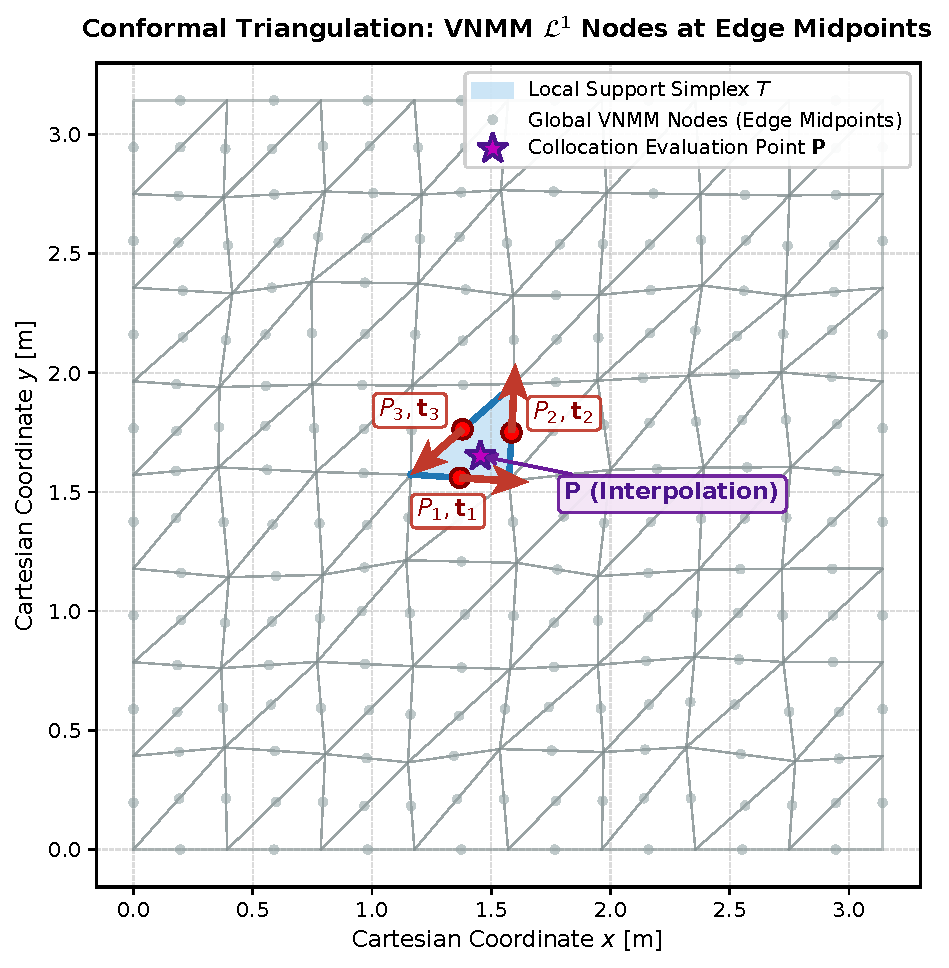
\includegraphics[width=\linewidth]{figura_malha_conforme_vnmm_L1.pdf}
    \caption{Conforming dual topology representation over the square domain $\Omega = [0, \pi] \times [0, \pi]$, displaying the underlying triangular finite element mesh alongside the dual VNMM $\mathcal{L}^1$ vector nodal cloud. Vector nodes are co-located at edge midpoints $M_k$ with unit directional vectors $\vec{t}_k$ aligned along the triangle edges. This exact midpoint co-location guarantees that support triads $\{P_1$, $P_2$, $P_3\}$ form local triangles matching the EFEM cells, establishing pointwise local dual equivalence.}
    \label{fig:malha_conforme_vnmm_L1}
\end{figure}

\subsubsection{Numerical Identity and Asymptotic Convergence Rates}
The asymptotic convergence behavior comparing the VNMM 2D $\mathcal{L}^1$ and Whitney EFEM formulations across the seven conforming mesh levels is presented in Fig.~\ref{fig:convergencia_efem_vs_vnmm_L1}.

As demonstrated in Fig.~\ref{fig:convergencia_efem_vs_vnmm_L1}a, the electric field RMS errors $\|\vec{E} - \vec{E}^h\|_{\mathrm{RMS}}$ for both formulations display an identical first-order asymptotic decay rate of $\mathcal{O}(h^{1.00})$. The point-by-point field difference between the two methods remains strictly bounded by double-precision floating-point machine precision, satisfying $\|\vec{E}^{\mathrm{VNMM}} - \vec{E}^{\mathrm{EFEM}}\|_{\mathrm{RMS}} \le 1.6 \times 10^{-16}$.

Similarly, Fig.~\ref{fig:convergencia_efem_vs_vnmm_L1}b illustrates the curl operator RMS error $\|(\nabla \times \vec{E})_z - (\nabla \times \vec{E}^h)_z\|_{\mathrm{RMS}}$, which exhibits an identical fitted convergence rate of $\mathcal{O}(h^{0.96})$ for both formulations. The mutual curl field difference is likewise bounded by machine precision, satisfying $\|(\nabla \times \vec{E})^{\mathrm{VNMM}} - (\nabla \times \vec{E})^{\mathrm{EFEM}}\|_{\mathrm{RMS}} \le 2.5 \times 10^{-15}$. These log-log convergence curves empirically confirm that the VNMM 2D $\mathcal{L}^1$ acts as the exact pointwise dual operator of Whitney 1-forms on conforming triangular cells.

\begin{figure}[!htbp]
    \centering
    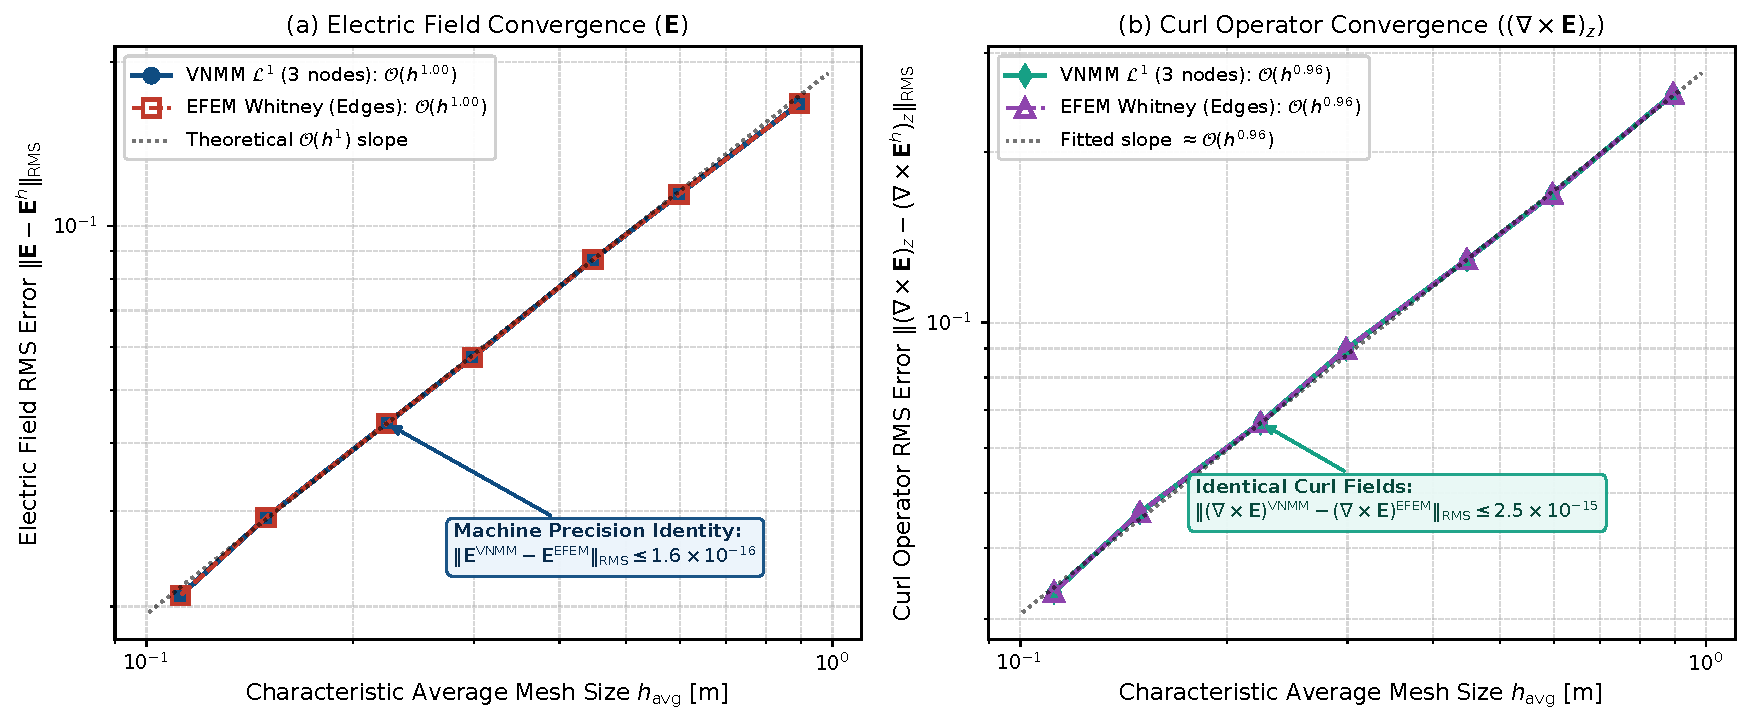
\includegraphics[width=\linewidth]{figura_convergencia_efem_vs_vnmm_L1.pdf}
    \caption{Asymptotic convergence rates comparing the Edge Finite Element Method (EFEM, Whitney 1-forms) and the Vector Nodal Meshless Method (VNMM $\mathcal{L}^1$, 3 support nodes) evaluated over the exact same conforming triangular mesh sequence: (a) electric field RMS error $\|\vec{E} - \vec{E}^h\|_{\mathrm{RMS}}$ exhibiting strictly identical $\mathcal{O}(h^{1.00})$ convergence with machine-precision difference $\|\vec{E}^{\mathrm{VNMM}} - \vec{E}^{\mathrm{EFEM}}\|_{\mathrm{RMS}} \le 1.6 \times 10^{-16}$; (b) curl operator RMS error $\|(\nabla \times \vec{E})_z - (\nabla \times \vec{E}^h)_z\|_{\mathrm{RMS}}$ displaying identical $\mathcal{O}(h^{0.96})$ convergence with mutual difference $\|(\nabla \times \vec{E})^{\mathrm{VNMM}} - (\nabla \times \vec{E})^{\mathrm{EFEM}}\|_{\mathrm{RMS}} \le 2.5 \times 10^{-15}$, confirming the exact constructive isomorphism between Whitney edge elements and VNMM $\mathcal{L}^1$.}
    \label{fig:convergencia_efem_vs_vnmm_L1}
\end{figure}

Crucially, this exact mathematical equivalence and global $H(\mathrm{curl})$ conformity hold \textbf{strictly under conforming mesh topologies} where support triads $\{P_1$, $P_2$, $P_3\}$ are constrained to edge midpoints of a well-defined cell. When transitioning to unconstrained, arbitrary meshless point clouds, support changes between evaluation points render the global approximation non-conforming (retaining local $H(\mathrm{curl})$ regularity within each local stencil), and this equivalence breaks down, as evaluated next.


\subsection{Vector Field Interpolation and Derivative Convergence in Arbitrary Meshless Clouds}
\label{subsec:arbitrary_meshless_interpolation}

While Section~\ref{subsec:conforming_dual_equivalence} established the exact pointwise equivalence between the incomplete 3-node basis $\mathcal{L}^1$ and Whitney 1-form edge elements on conforming triangular meshes, practical meshless modeling requires evaluating fields over unconstrained, non-conforming point clouds where vector nodes do not represent edge midpoints of an underlying triangulation \cite{goncalves2023vector, goncalves2025tese}. This subsection evaluates the asymptotic convergence behavior of the VNMM 2D under arbitrary spatial node distributions, validating the modal aliasing analysis presented in Section~\ref{subsec:L1_aliasing_analysis} and demonstrating its resolution via the 6-node linear polynomial vector space $\mathcal{P}^1$.
\subsubsection{Experimental Setup on Unconstrained Point Clouds}
The interpolation performance is assessed for the analytical $TE_{11}$ cavity mode specified in Eq.~\eqref{eq:analytical_te11_field} over unstructured, non-conforming nodal distributions covering $\Omega = [0, \pi] \times [0, \pi]$. Boundary nodes are placed uniformly along the domain perimeter with counterclockwise unit tangent vectors, whereas internal nodes are generated via a stratified Cartesian grid with $25\%$ stochastic spatial perturbation (\textit{jitter}) and random directional vector orientations $\mathbf{t}_k = [\cos\theta_k, \sin\theta_k]^T$.

To ensure strict statistical consistency, all field and derivative errors are evaluated across a fixed, invariant Cartesian grid of $1{,}600$ internal sampling points ($40 \times 40$) distributed uniformly in $[0.04\pi, 0.96\pi]^2$. The computational domain is discretized over six refinement levels, with node counts $N \in \{84$, $186$, $416$, $884$, $1{,}928$, $4{,}192\}$ and average nodal spacings ranging from $h_{\mathrm{avg}} = 0.5236$~m down to $0.0654$~m ($h_{\mathrm{avg}} \in \{0.52$, $0.35$, $0.22$, $0.15$, $0.10$, $0.07\}$~m).

\subsubsection{Empirical Validation of Curl Stagnation in \texorpdfstring{$\mathcal{L}^1$}{L1}}
When evaluated on unconstrained meshless clouds, the 3-node solenoidal basis $\mathcal{L}^1$ exhibits the fundamental breakdown in derivative convergence predicted theoretically in Section~\ref{subsec:L1_aliasing_analysis}. As illustrated by the log-log curves in Fig.~\ref{fig:convergencia_interpolacao_L1_vs_P1}a, the electric field RMS error $\|\vec{E} - \vec{E}^h\|_{\mathrm{RMS}}$ under $\mathcal{L}^1$ decreases monotonically at a first-order rate of $\mathcal{O}(h^{0.97})$, dropping from $1.91 \times 10^{-1}$ ($h = 0.5236$~m) down to $2.46 \times 10^{-2}$ ($h = 0.0654$~m).

However, as revealed in Fig.~\ref{fig:convergencia_interpolacao_L1_vs_P1}b, the RMS error of the curl operator $\|(\nabla \times \vec{E})_z - (\nabla \times \vec{E}^h)_z\|_{\mathrm{RMS}}$ \textbf{stagnates at an $\mathcal{O}(1)$ error plateau} ($\approx 0.85$, varying between $8.33 \times 10^{-1}$ and $8.88 \times 10^{-1}$, asymptotic rate $\mathcal{O}(h^{-0.01}) \approx \mathcal{O}(1)$), failing to converge under spatial refinement ($N = 4{,}192$). This persistent noise floor confirms the modal aliasing mechanism derived in Section~\ref{subsec:L1_aliasing_analysis}, wherein unrepresented normal field derivatives leak into the rotational coefficient via the inverted placement matrix $\mathbf{A}^{-1}$.
\begin{figure}[!htbp]
    \centering
    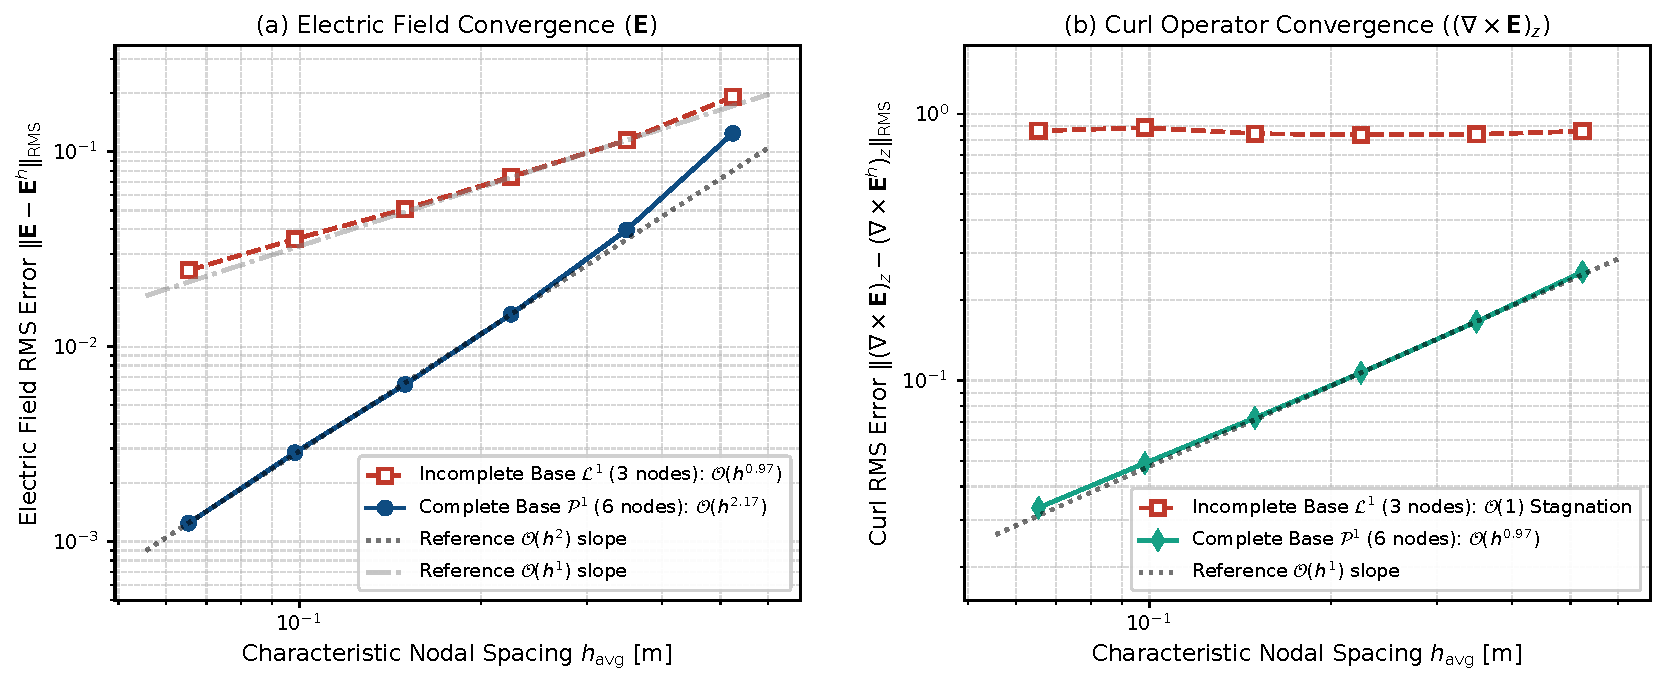
\includegraphics[width=\linewidth]{figura_convergencia_interpolacao_L1_vs_P1.pdf}
    \caption{Log-log convergence comparison between the incomplete Whitney-like base $\mathcal{L}^1$ (3 support nodes) and the complete linear base $\mathcal{P}^1$ (6 support nodes) over $\Omega = [0, \pi] \times [0, \pi]$ evaluated across a fixed Cartesian grid of $1{,}600$ internal points for the analytical $TE_{11}$ cavity mode: (a) electric field RMS error displaying standard $\mathcal{O}(h^{0.97})$ convergence for $\mathcal{L}^1$ versus an observed superconvergent rate of $\mathcal{O}(h^{2.17})$ for $\mathcal{P}^1$, delivering a $19.8\times$ error reduction on the finest grid ($h = 0.0654$~m); (b) curl operator RMS error demonstrating $\mathcal{O}(1)$ error stagnation for $\mathcal{L}^1$ (plateau at $\approx 0.85$ due to missing cross-derivatives), in contrast to asymptotic $\mathcal{O}(h^{0.97})$ convergence for $\mathcal{P}^1$, yielding a $25.9\times$ error reduction.}
    \label{fig:convergencia_interpolacao_L1_vs_P1}
\end{figure}

\subsubsection{Restoration of Asymptotic Convergence via Complete \texorpdfstring{$\mathcal{P}^1$}{P1} Basis}
Expanding the local approximation space to the complete linear polynomial vector space $\mathcal{P}^1$ introduced in Section~\ref{subsec:complete_P1_basis} provides six independent degrees of freedom, capturing all four components of the local Jacobian tensor $\nabla\vec{E}^h$. Local support domains (averaging $K_{\mathrm{avg}} \approx 11.0$ neighbors, ranging from $10.7$ to $11.2$) are selected via $k$-d tree spatial searches subject to the adaptive quartic determinant threshold developed in Section~\ref{sec:support_selection_algorithm}.

As demonstrated in Fig.~\ref{fig:convergencia_interpolacao_L1_vs_P1}, transitioning to $\mathcal{P}^1$ removes derivative modal aliasing and achieves two major performance gains:
\begin{enumerate}
    \item \textbf{Observed Superconvergence for Field $\vec{E}^h$ (Fig.~\ref{fig:convergencia_interpolacao_L1_vs_P1}a):} Completing the linear polynomial space elevates the observed electric field convergence rate from $\mathcal{O}(h^{0.97})$ to approximately quadratic $\mathcal{O}(h^{2.17})$. At the finest discretization ($h = 0.0654$~m), the field RMS error drops from $2.46 \times 10^{-2}$ ($\mathcal{L}^1$) down to $1.24 \times 10^{-3}$ ($\mathcal{P}^1$), representing a \textbf{$19.8\times$ precision gain}. We emphasize that while the restoration of first-order curl convergence is a direct mathematical consequence of resolving the complete local Jacobian and eliminating derivative modal aliasing, the observed superconvergent rate $\mathcal{O}(h^{2.17})$ for the electric field is an empirical finding on the tested analytical $TE_{11}$ cavity benchmark. The theoretical origin of this superconvergence and its formal extension to arbitrary geometries and field profiles remain an open question for future mathematical analysis.
    \item \textbf{Restoration of Asymptotic $\mathcal{O}(h^1)$ Curl Convergence (Fig.~\ref{fig:convergencia_interpolacao_L1_vs_P1}b):} By accommodating normal derivatives in the Taylor expansion, the complete $\mathcal{P}^1$ basis restores first-order convergence $\mathcal{O}(h^{0.97})$ for the curl operator. The curl RMS error decreases monotonically from $2.55 \times 10^{-1}$ down to $3.33 \times 10^{-2}$ at $h = 0.0654$~m, delivering a \textbf{$25.9\times$ error reduction} over the stagnated $\mathcal{L}^1$ formulation ($8.63 \times 10^{-1}$).
\end{enumerate}

Consequently, while $\mathcal{L}^1$ is suitable for conforming triangular meshes where circulation cancellation holds (Section~\ref{subsec:conforming_dual_equivalence}), adopting the complete $\mathcal{P}^1$ vector space is sufficient to eliminate the derivative-aliasing mechanism and restore first-order curl convergence across unconstrained, arbitrary meshless point clouds. The quantitative performance comparison between the two bases across all six refinement levels is detailed in Table~\ref{tab:interpolacao_L1_vs_P1}.

\begin{table}[!htbp]
\centering
\caption{Comparative vector interpolation error metrics and asymptotic convergence between the incomplete base $\mathcal{L}^1$ (3 support nodes) and complete base $\mathcal{P}^1$ (6 support nodes) over $\Omega = [0, \pi] \times [0, \pi]$ evaluated across a fixed grid of $1{,}600$ internal points for the analytical $TE_{11}$ cavity mode.}
\label{tab:interpolacao_L1_vs_P1}
\resizebox{\columnwidth}{!}{%
\begin{tabular}{@{} c c c c c c c c c @{}}
\toprule
$N_{\mathrm{total}}$ & $h_{\mathrm{avg}}$ [m] & \multicolumn{3}{c}{\textbf{Electric Field RMS Error}} & \multicolumn{3}{c}{\textbf{Curl Operator RMS Error}} & $K_{\mathrm{avg}}$ \\
\cmidrule(lr){3-5} \cmidrule(lr){6-8}
& & $\mathcal{L}^1$ & $\mathcal{P}^1$ & \textbf{Gain} & $\mathcal{L}^1$ & $\mathcal{P}^1$ & \textbf{Gain} & ($\mathcal{P}^1$) \\
\midrule
84   & 0.5236 & $1.91 \times 10^{-1}$ & $1.24 \times 10^{-1}$ & $\mathbf{1.5\times}$  & $8.61 \times 10^{-1}$ & $2.55 \times 10^{-1}$ & $\mathbf{3.4\times}$  & 11.1 \\
186  & 0.3491 & $1.15 \times 10^{-1}$ & $3.97 \times 10^{-2}$ & $\mathbf{2.9\times}$  & $8.38 \times 10^{-1}$ & $1.66 \times 10^{-1}$ & $\mathbf{5.0\times}$  & 11.2 \\
416  & 0.2244 & $7.44 \times 10^{-2}$ & $1.47 \times 10^{-2}$ & $\mathbf{5.1\times}$  & $8.34 \times 10^{-1}$ & $1.07 \times 10^{-1}$ & $\mathbf{7.8\times}$  & 11.2 \\
884  & 0.1496 & $5.08 \times 10^{-2}$ & $6.39 \times 10^{-3}$ & $\mathbf{7.9\times}$  & $8.43 \times 10^{-1}$ & $7.24 \times 10^{-2}$ & $\mathbf{11.6\times}$ & 10.9 \\
1{,}928 & 0.0982 & $3.56 \times 10^{-2}$ & $2.86 \times 10^{-3}$ & $\mathbf{12.5\times}$ & $8.88 \times 10^{-1}$ & $4.89 \times 10^{-2}$ & $\mathbf{18.1\times}$ & 10.9 \\
4{,}192 & 0.0654 & $2.46 \times 10^{-2}$ & $1.24 \times 10^{-3}$ & $\mathbf{19.8\times}$ & $8.63 \times 10^{-1}$ & $3.33 \times 10^{-2}$ & $\mathbf{25.9\times}$ & 10.7 \\
\midrule
\multicolumn{2}{c}{\textbf{Fitted Rate}} & $\mathcal{O}(h^{0.97})$ & $\mathbf{\mathcal{O}(h^{2.17})}$ & --- & $\mathcal{O}(h^{-0.01})$ & $\mathbf{\mathcal{O}(h^{0.97})}$ & --- & --- \\
\bottomrule
\end{tabular}%
}
\end{table}

% ---------------------------------------------------------
% SUBSECTION 6.3: NUMERICAL STABILITY UNDER STOCHASTIC PERTURBATIONS
% ---------------------------------------------------------
\subsection{Numerical Robustness in the Tested Stochastic Realization Under Spatial-Directional Perturbations}
\label{subsec:stochastic_perturbations}

While Section~\ref{subsec:arbitrary_meshless_interpolation} demonstrated that the complete $\mathcal{P}^1$ space successfully eliminates derivative modal aliasing and restores asymptotic curl convergence, practical meshless computing on arbitrary unstructured point clouds demands evaluating the algebraic stability of the support qualification algorithm itself \cite{slak2018refined}. In unconstrained clouds, arbitrary spatial arrangements and director orientations can induce pathological local configurations---such as near-parallel directors ($\ge 4$ parallel nodes) or near-collinear nodes ($\ge 5$ collinear nodes)---that degrade the conditioning of the local placement matrix $\mathbf{A} \in \mathbb{R}^{6 \times 6}$ (Section~\ref{subsec:singularities_P1}).

To evaluate the stabilization mechanism provided by the scale-dependent determinant thresholding law with an absolute floor (Eq.~\eqref{eq:scale_dependent_determinant_floor}, Section~\ref{sec:support_selection_algorithm}) within the complete $\mathcal{P}^1$ basis over $\Omega = [0, \pi] \times [0, \pi]$, we subject the point cloud sequence to a representative benchmark scenario combining simultaneous stochastic spatial-directional distortions ($25\%$ spatial jitter and random director orientations):
\begin{enumerate}
    \item \textbf{Stochastic Spatial Jitter:} Interior node coordinates are perturbed as $\mathbf{x}_k \leftarrow \mathbf{x}_k + \delta\mathbf{x}_k$, with independent random displacements $\delta x_k$, $\delta y_k \sim \mathcal{U}(-0.25\,\Delta x, 0.25\,\Delta x)$, introducing a $25\%$ random spatial jitter relative to the base lattice spacing.
    \item \textbf{Random Unit Director Orientations:} Unit vector directors assigned to interior nodes receive fully random angles $\theta_k \sim \mathcal{U}(0, 2\pi)$, defining $\vec{t}_k = [\cos\theta_k, \sin\theta_k]^T$, completely removing directional alignment symmetry.
\end{enumerate}

Although extensive Monte Carlo characterization across multi-seed ensembles remains future work, this benchmark sequence provides a representative stochastic stress test for the automated qualification pipeline, assessing whether the scale-dependent determinant threshold can dynamically detect and bypass localized pathological candidate sextets without manual intervention. Figure~\ref{fig:robustez_perturbacao_estocastica} illustrates the resulting convergence behavior and parametric sensitivity analysis comparing the unconstrained pure quartic scaling law against the stabilized formulation with an absolute determinant floor.

\begin{figure*}[!t]
\centering
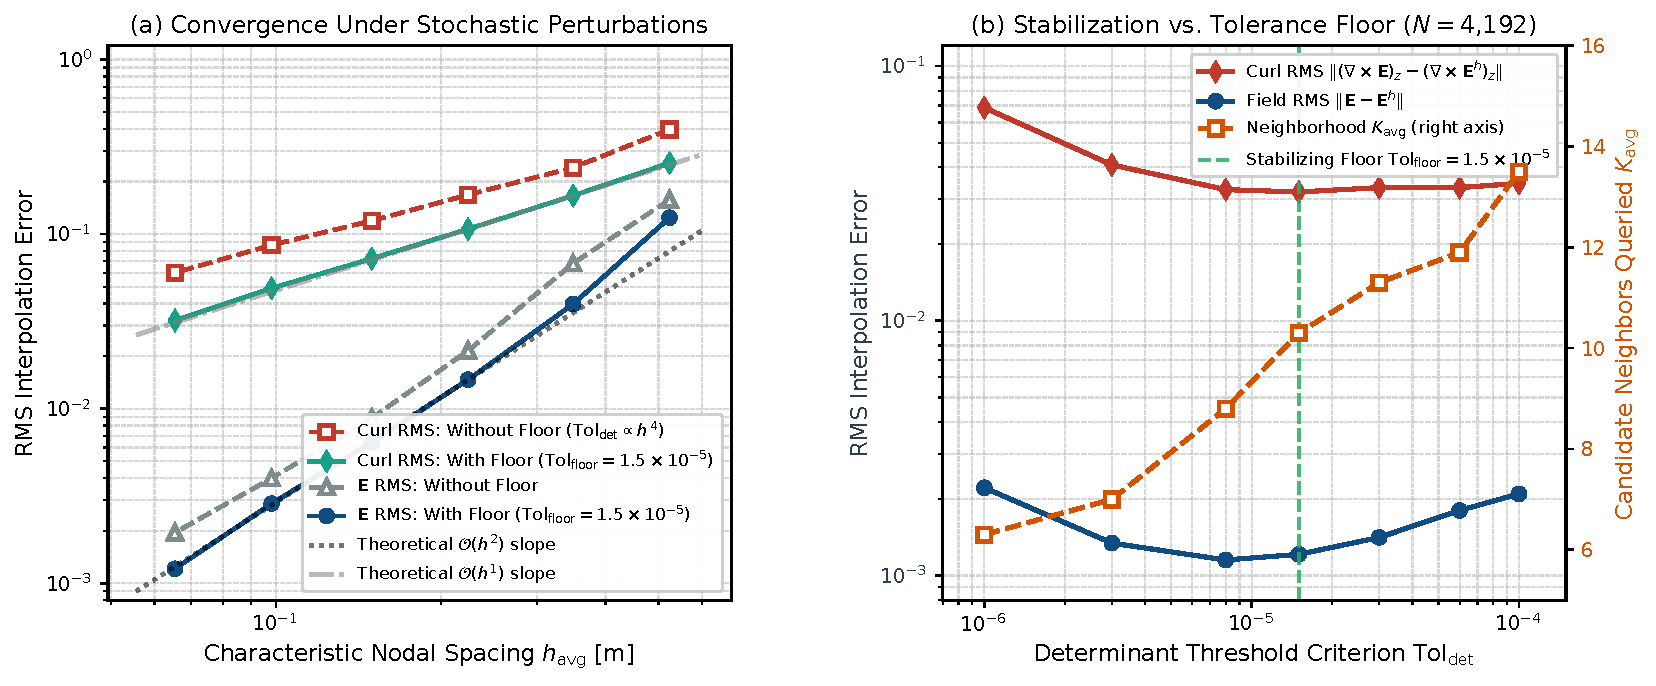
\includegraphics[width=0.98\textwidth]{figura_robustez_perturbacao_estocastica.pdf}
\caption{Numerical robustness and conditioning analysis in the tested stochastic realization for the 2D VNMM complete base $\mathcal{P}^1$ under spatial-directional perturbations (uniform nodal jitter of $25\%$ and random director angles $\theta_i \in [0, 2\pi)$) over $\Omega = [0, \pi]^2$: (a) Convergence under stochastic mesh refinement with and without the determinant tolerance floor, highlighting curl degradation when scaling $\mathrm{Tol}_{\mathrm{det}} \propto h^4$ without a floor due to ill-conditioned sextets ($\kappa(\mathbf{A}) > 180$) and restored strict monotonic convergence when applying $\mathrm{Tol}_{\mathrm{floor}} = 1.5 \times 10^{-5}$; (b) Interpolation error and candidate search neighborhood $K_{\mathrm{avg}}$ as a function of the threshold criterion $\mathrm{Tol}_{\mathrm{det}}$ for the fine grid ($N = 4{,}192$), identifying the stable operating regime for $\mathrm{Tol}_{\mathrm{det}} \ge 1.5 \times 10^{-5}$.}
\label{fig:robustez_perturbacao_estocastica}
\end{figure*}

\subsubsection{Failure of the Pure Quartic Scaling Law in Dense Perturbed Clouds}
\label{subsubsec:quartic_law_failure}

As established in Section~\ref{subsec:singularities_P1}, placement matrix columns 3--6 in the complete $\mathcal{P}^1$ basis scale linearly with local node spacing as $\mathcal{O}(h)$, causing the local placement determinant to scale quartically as $\det(\mathbf{A}_{6 \times 6}) \sim \mathcal{O}(h^4)$. When employing a pure unconstrained scaling law $\mathrm{Tol}_{\mathrm{det}}^{\mathrm{pure}}(h) \propto h^4$, the determinant acceptance threshold drops precipitously in dense grids, reaching $\mathrm{Tol}_{\mathrm{det}} \approx 1.2 \times 10^{-6}$ at $h = 0.0654$\,m ($N = 4{,}192$).

Under stochastic spatial-directional noise, this unconstrained drop causes numerical instability:
\begin{itemize}
    \item At $\mathrm{Tol}_{\mathrm{det}} \le 1.2 \times 10^{-6}$, the early-stopping qualification accepts the immediate 6 nearest spatial neighbors ($K_{\mathrm{avg}} \approx 6.3$).
    \item Because node coordinates and directors are stochastically perturbed, these immediate spatial neighbors frequently form ill-conditioned sextets approaching the singularity modes analyzed in Section~\ref{subsec:singularities_P1} (e.g., 4 near-parallel directors or 5 near-collinear nodes), elevating the matrix condition number to $\kappa(\mathbf{A}) > 180$.
    \item Because spatial derivatives scale dimensionally as $\mathcal{O}(h^{-1})$, the ill-conditioned inverted matrix $\mathbf{A}^{-1}$ amplifies local interpolation errors. As shown by the dashed crimson curve in Fig.~\ref{fig:robustez_perturbacao_estocastica}a, this causes the curl operator RMS error to flatten and stagnate as $h \to 0.0654$~m, remaining elevated at an RMS error of $\approx 6.01 \times 10^{-2}$ to $8.66 \times 10^{-2}$ for $(\nabla \times \vec{E}^h)_z$.
\end{itemize}

\subsubsection{Restoration of Monotonicity via Absolute Tolerance Floor}
\label{subsubsec:restoration_via_floor}

Enforcing the absolute lower bound $\mathrm{Tol}_{\mathrm{floor}} = 1.5 \times 10^{-5}$ in the scale-dependent law (Eq.~\eqref{eq:scale_dependent_determinant_floor}, Section~\ref{sec:support_selection_algorithm}) mitigates this derivative instability.

As demonstrated by the solid teal curves in Fig.~\ref{fig:robustez_perturbacao_estocastica}a, when $h \to 0.0654$\,m, the lower bound $\mathrm{Tol}_{\mathrm{floor}} = 1.5 \times 10^{-5}$ overrides the decaying quartic threshold. This forces the $k$-d tree candidate search to expand its local sampling radius moderately ($K_{\mathrm{avg}}$ expands from $6.3$ to $10.3$), automatically skipping near-collinear or near-parallel neighbor combinations that violate the determinant floor. By dynamically identifying an admissible support under the tested thresholding strategy via the 4-phase selection algorithm (Section~\ref{subsec:4phase_pipeline}), the method restores monotonic error reduction across the tested refinement range for both field $\vec{E}^h$ and curl $(\nabla \times \vec{E}^h)_z$, reducing curl error to $3.20 \times 10^{-2}$ on the finest mesh ($N = 4{,}192$).

\subsubsection{Parametric Neighborhood Trade-off and Stabilization Threshold}
\label{subsubsec:parametric_tradeoff}

To identify the best-performing compromise between conditioning, curl error, and neighborhood size on $\Omega = [0, \pi]^2$, a systematic parametric sweep was conducted on the stochastically perturbed fine grid ($N = 4{,}192, h = 0.0654$\,m) across determinant thresholds ranging from $\mathrm{Tol}_{\mathrm{det}} = 1.0 \times 10^{-6}$ up to $1.0 \times 10^{-4}$. The quantitative results are summarized in Table~\ref{tab:stochastic_sensitivity_ultradense}.

\begin{table}[!htbp]
\centering
\caption{Parametric error sensitivity, support neighborhood size $K_{\mathrm{avg}}$, and placement matrix conditioning as a function of determinant threshold $\mathrm{Tol}_{\mathrm{det}}$ for the stochastically perturbed fine grid ($N = 4{,}192, h = 0.0654$\,m) over $\Omega = [0, \pi]^2$.}
\label{tab:stochastic_sensitivity_ultradense}
\resizebox{\columnwidth}{!}{%
\begin{tabular}{@{} c c c c c c @{}}
\toprule
\textbf{Threshold} & \textbf{Success} & \textbf{Neighbors} & \multicolumn{2}{c}{\textbf{RMS Error}} & \textbf{Conditioning} \\
\cmidrule(lr){4-5}
$\mathrm{Tol}_{\mathrm{det}}$ & \textbf{Rate} & $K_{\mathrm{avg}}$ & $\vec{E}^h$ & $(\nabla\times\vec{E}^h)_z$ & $\kappa_2(\mathbf{A})$ \\
\midrule
\begin{tabular}[c]{@{}c@{}} $1.0 \times 10^{-6}$ \\ \scriptsize(Permissive) \end{tabular} & 100\% & 6.3 & $2.21 \times 10^{-3}$ & $6.86 \times 10^{-2}$ & \begin{tabular}[c]{@{}c@{}} $> 180$ \\ \scriptsize(Sub-cond.) \end{tabular} \\
$3.0 \times 10^{-6}$ & 100\% & 7.0 & $1.34 \times 10^{-3}$ & $4.09 \times 10^{-2}$ & $\approx 141$ \\
$8.0 \times 10^{-6}$ & 100\% & 8.8 & $1.15 \times 10^{-3}$ & $3.27 \times 10^{-2}$ & $\approx 99$ \\
\begin{tabular}[c]{@{}c@{}} $\mathbf{1.5 \times 10^{-5}}$ \\ \scriptsize\textbf{(Floor)} \end{tabular} & 100\% & \textbf{10.3} & $\mathbf{1.21 \times 10^{-3}}$ & $\mathbf{3.20 \times 10^{-2}}$ & \begin{tabular}[c]{@{}c@{}} $\mathbf{\approx 73}$ \\ \scriptsize\textbf{(Stable)} \end{tabular} \\
\begin{tabular}[c]{@{}c@{}} $\mathbf{3.0 \times 10^{-5}}$ \\ \scriptsize\textbf{(Compromise)} \end{tabular} & 100\% & \textbf{11.3} & $\mathbf{1.41 \times 10^{-3}}$ & $\mathbf{3.33 \times 10^{-2}}$ & \begin{tabular}[c]{@{}c@{}} $\mathbf{\approx 64}$ \\ \scriptsize\textbf{(Stable)} \end{tabular} \\
$6.0 \times 10^{-5}$ & 100\% & 11.9 & $1.80 \times 10^{-3}$ & $3.33 \times 10^{-2}$ & $\approx 61$ \\
$1.0 \times 10^{-4}$ & 100\% & 13.5 & $2.09 \times 10^{-3}$ & $3.46 \times 10^{-2}$ & $\approx 58$ \\
\bottomrule
\end{tabular}%
}
\end{table}

As illustrated in Fig.~\ref{fig:robustez_perturbacao_estocastica}b:
\begin{enumerate}
    \item \textbf{Stabilization Zone ($\mathrm{Tol}_{\mathrm{floor}} \ge 1.5 \times 10^{-5}$):} Increasing $\mathrm{Tol}_{\mathrm{det}}$ from $1.0 \times 10^{-6}$ to $1.5 \times 10^{-5}$ produces a sharp, monotonic reduction in curl interpolation error (a $2.1\times$ precision gain from $6.86 \times 10^{-2}$ down to $3.20 \times 10^{-2}$), while bounding matrix conditioning to $\kappa_2(\mathbf{A}) \le 73$ at the operational baseline floor $\mathrm{Tol}_{\mathrm{floor}} = 1.5 \times 10^{-5}$ and decreasing to $\approx 64$ at the compromise threshold $\mathrm{Tol}_{\mathrm{det}} = 3.0 \times 10^{-5}$.
    \item \textbf{Compact Support Locality and Trade-off ($K_{\mathrm{avg}} \le 11.3$):} This precision gain requires expanding the candidate search neighborhood from $K_{\mathrm{avg}} = 6.3$ to only $K_{\mathrm{avg}} = 10.3$ (at the floor) and $11.3$ (at the compromise threshold). While larger thresholds ($\mathrm{Tol}_{\mathrm{det}} \ge 6.0 \times 10^{-5}$) further reduce $\kappa_2(\mathbf{A})$ to $\approx 58\text{--}61$, they do so at the cost of larger neighborhood pools ($K_{\mathrm{avg}} \to 13.5$) and elevated field interpolation errors, establishing $\mathrm{Tol}_{\mathrm{det}} = 3.0 \times 10^{-5}$ (along with the operational floor $1.5 \times 10^{-5}$) as the best-performing compromise between conditioning, curl error, and neighborhood size. Crucially, this compact neighborhood size matches that of unperturbed clouds ($K_{\mathrm{avg}} \approx 11.0$, Table~\ref{tab:interpolacao_L1_vs_P1}), demonstrating that the absolute tolerance floor effectively suppresses directional collinearities without unphysical support dilation, thereby preserving spatial search efficiency and compact support locality without combinatorial overhead (Section~\ref{subsubsec:computational_complexity}).
\end{enumerate}

While this benchmark demonstrates the mechanical action of the determinant floor across an individual perturbed refinement sequence, a full Monte Carlo characterization involving ensembles of tens of stochastic realizations per refinement level constitutes an important avenue for future statistical validation of generalized unstructured cloud generators.


% ---------------------------------------------------------
% SUBSECTION 6.3: RESONANT CAVITY SPECTRAL ANALYSIS AND DIV-CURL REGULARIZATION
% ---------------------------------------------------------
\subsection{Spectral Validation: Resonant Cavity Analysis and Div-Curl Regularization}
\label{subsec:cavity_eigenvalues}
Having established the variational framework for the electromagnetic vector eigenvalue problem in Section~\ref{sec:variational_formulation}, this experiment evaluates the spectral accuracy of the Vector Nodal Meshless Method (VNMM 2D) and verifies the suppression of non-physical spurious modes across the operational frequency band. Numerical simulations are conducted for Transverse Electric ($TE_z$) modes over the square PEC cavity using the complete $\mathcal{P}^1$ basis, comparing discrete spectra against the analytical reference eigenvalues defined in Eq.~\eqref{eq:analytical_eigenvalues}.

Figure~\ref{fig:espectro_cavidade_regularizacao} presents the discrete eigenvalue spectra ($\lambda = k_c^2$), contrasting the unregularized formulation against the div-curl regularized formulation ($s_{\mathrm{div}} = 6.0$) developed in Eq.~\eqref{eq:regularized_weak_form}.

\begin{figure}[!htbp]
    \centering
    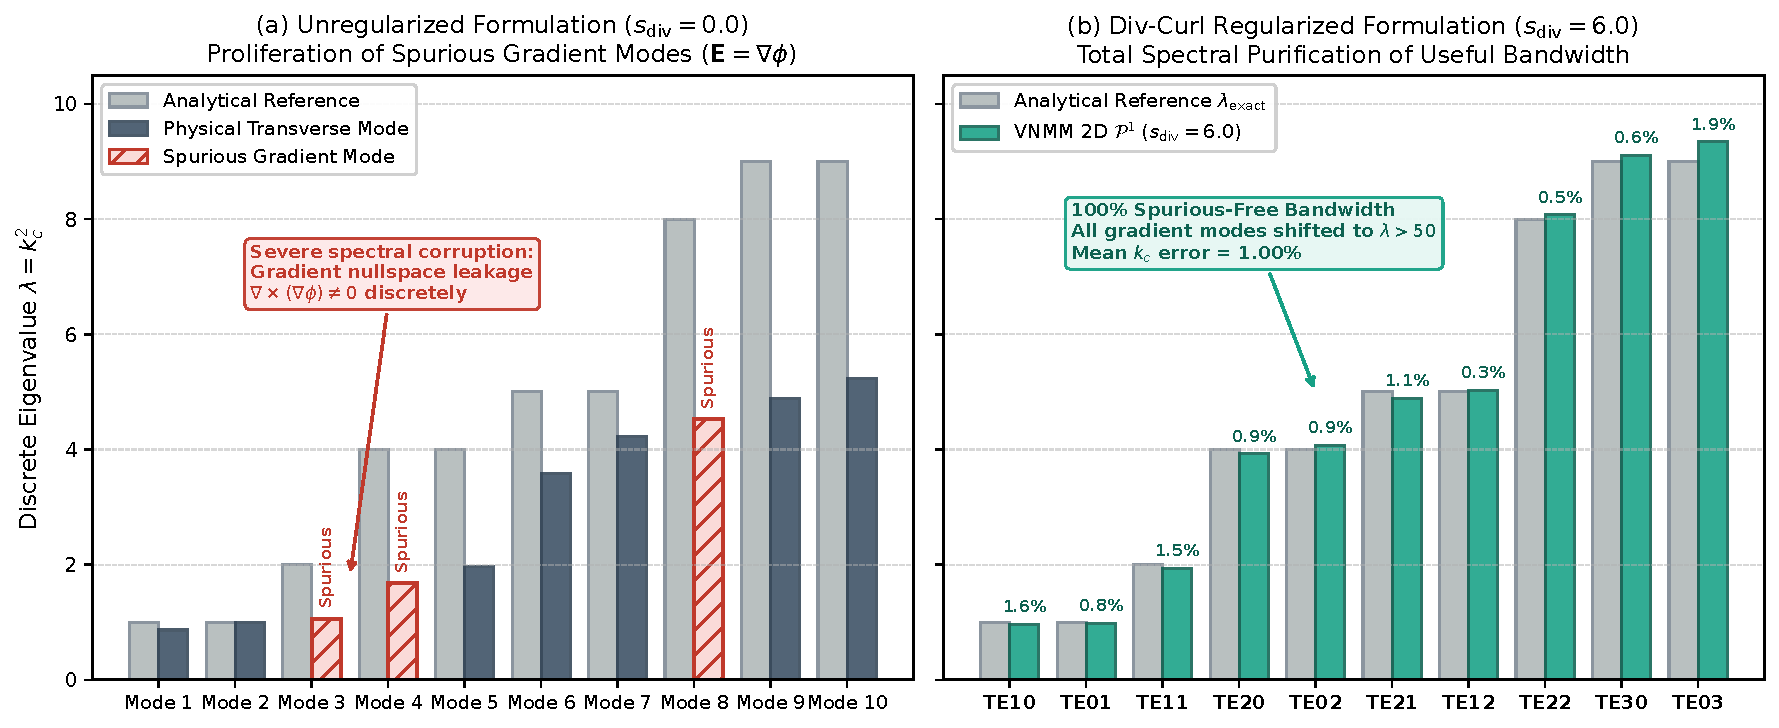
\includegraphics[width=\linewidth]{figura_espectro_cavidade_com_sem_regularizacao.pdf}
    \caption{Discrete eigenvalue spectrum $\lambda = k_c^2$ for the $TE_z$ square PEC cavity: (a) Unregularized curl-curl formulation ($s_{\mathrm{div}} = 0.0$), illustrating the severe spectral contamination caused by discrete gradient nullspace leakage ($\nabla \times (\nabla \phi) \neq \mathbf{0}$), where non-zero spurious modes infiltrate the physical sequence; (b) Div-curl regularized formulation ($s_{\mathrm{div}} = 6.0$), demonstrating effective spectral purification across the useful physical bandwidth with no spurious modes observed among the tested resonances, shifting gradient modes to $\lambda > 50$ for the tested cavity discretization and restricting the mean cutoff wavenumber error to $1.00\%$.}
    \label{fig:espectro_cavidade_regularizacao}
\end{figure}

Numerical evaluations are conducted on the base-case regular discretization with $N_x = 21, N_y = 21$ ($N_{\mathrm{total}} = 441$ nodes, yielding $M_{\mathrm{active}} = 361$ internal degrees of freedom after enforcing homogeneous tangential PEC boundary conditions $c_k = 0$ on $\partial\Omega$). The weak form integrals are computed over a background grid of $10 \times 10$ quadrilateral cells ($N_c = 100$) using $2 \times 2$ Gauss-Legendre quadrature (400 Gauss points), maintaining a suitable quadrature-to-DoF ratio ($N_g / N_{\mathrm{DoF}} \approx 1.11$) \cite{belytschko1994element, liu2005introduction, liu2009mesh}.

\subsubsection{Spectral Contamination in the Unregularized Curl-Curl Formulation (\texorpdfstring{$s_{\mathrm{div}} = 0.0$}{s_div = 0.0})}
\label{subsubsec:unregularized_formulation}

As analyzed theoretically in Section~\ref{subsec:weak_form_regularization}, point-collocated meshless vector shape functions fail to form an exact discrete de Rham complex at background quadrature points. Unlike Edge Finite Element Methods (EFEM) that achieve closed-contour circulation cancellation, discrete gradient fields in unregularized meshless formulations generate non-zero numerical curl residues ($\nabla \times (\nabla \phi) \neq \mathbf{0}$ at Gauss points).

The empirical impact of this nullspace leakage is clearly observed in Fig.~\ref{fig:espectro_cavidade_regularizacao}a. Setting $s_{\mathrm{div}} = 0.0$ transforms analytical zero-eigenvalues belonging to $\ker(\nabla \times)$ into small, positive non-zero states ($0.8 < \lambda < 5.0$). These non-physical spurious gradient modes infiltrate the physical $TE_z$ sequence, corrupting modal ordering and elevating the mean relative cutoff wavenumber error to unacceptable levels ($19.75\%$ to $90.0\%$).

\subsubsection{Spectral Purification via Div-Curl Penalty Regularization (\texorpdfstring{$s_{\mathrm{div}} = 6.0$}{s_div = 6.0})}
\label{subsubsec:regularized_formulation}

To eliminate the non-physical spurious gradient modes identified in Section~\ref{subsubsec:unregularized_formulation} without introducing auxiliary Lagrange multipliers or expanding the system matrix, the div-curl variational penalty parameter is activated with $s_{\mathrm{div}} = 6.0$ in Eq.~\eqref{eq:regularized_weak_form}.

As established in Section~\ref{subsec:weak_form_regularization}, the divergence penalty matrix $\mathbf{K}_{\mathrm{div}}$ operates selectively between physical and spurious subspaces. While physical $TE_z$ cavity modes are divergence-free at the continuous level, discrete approximation residues ($\nabla \cdot \vec{E}^h \sim \mathcal{O}(h)$) generate only a minor eigenvalue perturbation that decreases with refinement, with the divergence-to-curl energy ratio remaining bounded at $R_{\mathrm{div}} = \frac{\mathbf{c}^T \mathbf{K}_{\mathrm{div}} \mathbf{c}}{\mathbf{c}^T \mathbf{K}_{\mathrm{curl}} \mathbf{c}} \sim 10^{-3} \text{--} 10^{-2}$ for the first 10 physical modes (and decaying monotonically as $R_{\mathrm{div}} \propto h$ under refinement). In contrast, for non-physical gradient states ($\vec{E} = \nabla \phi$), this ratio reaches $R_{\mathrm{div}} \sim 10^3 \text{--} 10^4$ in the unregularized system; for the tested cavity discretization and choice of $s_{\mathrm{div}} = 6.0$, this imparts immense artificial numerical stiffness that shifts the discrete non-physical gradient states outside the operational frequency window of the tested setup ($\lambda > 50$).

The experimental confirmation of this selective purification is demonstrated in Fig.~\ref{fig:espectro_cavidade_regularizacao}b. Activating $s_{\mathrm{div}} = 6.0$ ensures that no spurious modes are detected among the first ten computed resonances within the tested operational spectral window ($\lambda \le 10$), removing non-physical gradient branches from the low-frequency discrete spectrum and restoring 1-to-1 modal correspondence with the analytical reference eigenvalues defined in Eq.~\eqref{eq:analytical_eigenvalues}.

\subsubsection{Modewise Validation and Cutoff Wavenumber Precision}
\label{subsubsec:modewise_validation}

The numerical performance of the regularized VNMM 2D ($\mathcal{P}^1$, $s_{\mathrm{div}} = 6.0$) for the first 10 physical $TE_{nm}$ cavity modes is detailed in Table~\ref{tab:cavity_eigenvalues_base_case}.

\begin{table}[!htbp]
\centering
\caption{Comparison of the first 10 physical $TE_{nm}$ resonant modes in the square PEC cavity $\Omega = [0, \pi]^2$ between analytical reference values and the proposed regularized VNMM 2D formulation ($\mathcal{P}^1$, $s_{\mathrm{div}} = 6.0$, $361$ active DoFs).}
\label{tab:cavity_eigenvalues_base_case}
\resizebox{\columnwidth}{!}{%
\begin{tabular}{@{} c c c c c c c @{}}
\toprule
\textbf{Mode ($TE_{nm}$)} & $\lambda_{\mathrm{analytical}}$ & $k_{c, \mathrm{analytical}}$ & $\lambda_{\mathrm{VNMM}}$ & $k_{c, \mathrm{VNMM}}$ & \textbf{Error $\lambda$ (\%)} & \textbf{Error $k_c$ (\%)} \\
\midrule
$TE_{10}$ & $1.00$ & $1.000$ & $0.9679$ & $0.984$ & $3.21\%$ & $\mathbf{1.62\%}$ \\
$TE_{01}$ & $1.00$ & $1.000$ & $0.9836$ & $0.992$ & $1.64\%$ & $\mathbf{0.82\%}$ \\
$TE_{11}$ & $2.00$ & $1.414$ & $1.9409$ & $1.393$ & $2.95\%$ & $\mathbf{1.49\%}$ \\
$TE_{20}$ & $4.00$ & $2.000$ & $3.9275$ & $1.982$ & $1.81\%$ & $\mathbf{0.91\%}$ \\
$TE_{02}$ & $4.00$ & $2.000$ & $4.0724$ & $2.018$ & $1.81\%$ & $\mathbf{0.90\%}$ \\
$TE_{21}$ & $5.00$ & $2.236$ & $4.8925$ & $2.212$ & $2.15\%$ & $\mathbf{1.08\%}$ \\
$TE_{12}$ & $5.00$ & $2.236$ & $5.0287$ & $2.242$ & $0.57\%$ & $\mathbf{0.29\%}$ \\
$TE_{22}$ & $8.00$ & $2.828$ & $8.0743$ & $2.842$ & $0.93\%$ & $\mathbf{0.46\%}$ \\
$TE_{30}$ & $9.00$ & $3.000$ & $9.1089$ & $3.018$ & $1.21\%$ & $\mathbf{0.60\%}$ \\
$TE_{03}$ & $9.00$ & $3.000$ & $9.3409$ & $3.056$ & $3.79\%$ & $\mathbf{1.88\%}$ \\
\midrule
\textbf{Global Mean} & --- & --- & --- & --- & $\mathbf{2.01\%}$ & $\mathbf{1.00\%}$ \\
\bottomrule
\end{tabular}%
}
\end{table}

The regularized VNMM 2D achieves a global mean cutoff wavenumber error of $1.00\%$ (with a maximum error of $1.88\%$ for the $TE_{03}$ mode), strictly matching analytical degeneracies ($TE_{10}/TE_{01}$, $TE_{20}/TE_{02}$, $TE_{21}/TE_{12}$, $TE_{30}/TE_{03}$) without spurious mode infiltration. Importantly, parametric sensitivity evaluations confirm that this spectral purification is highly robust across a wide penalty window $s_{\mathrm{div}} \in [4.0, 10.0]$, verifying that the formulation does not require delicate, problem-dependent parameter tuning.

\subsubsection{Sensitivity to Background Cell Density and Gauss Quadrature Order}
\label{subsubsec:quadrature_sensitivity}

To address the dependency on background integration scaffolding and assess the sensitivity of spectral predictions to quadrature resolution, we conduct a parametric sensitivity analysis over the base cavity discretization ($N = 21 \times 21$, $361$ active DoFs). Table~\ref{tab:quadrature_sensitivity} details the resulting mean and maximum cutoff wavenumber errors, relative Frobenius matrix differences against an ultra-refined reference integration ($\mathbf{K}_{\mathrm{ref}}, \mathbf{M}_{\mathrm{ref}}$ computed on $40 \times 40$ cells with $4 \times 4$ Gauss points, $N_g = 25{,}600$), and global assembly times.

\begin{table}[!htbp]
\centering
\caption{Sensitivity of resonant cavity spectral accuracy, discrete operator convergence, and assembly cost to background cell discretization and Gauss quadrature order ($N = 21 \times 21$, $361$ active DoFs, $s_{\mathrm{div}} = 6.0$, reference grid: $40 \times 40$ cells, $4 \times 4$ Gauss).}
\label{tab:quadrature_sensitivity}
\resizebox{\columnwidth}{!}{%
\begin{tabular}{@{} c c c c c c c c @{}}
\toprule
\textbf{Background Grid} & \textbf{Gauss Rule} & \textbf{Gauss Pts} & \multicolumn{2}{c}{\textbf{Wavenumber Error}} & \multicolumn{2}{c}{\textbf{Relative Matrix Difference}} & \textbf{Assembly} \\
\cmidrule(lr){4-5} \cmidrule(lr){6-7}
($N_{cx} \times N_{cy}$) & ($p \times p$) & ($N_g$) & \textbf{Mean $k_c$ (\%)} & \textbf{Max $k_c$ (\%)} & $\frac{\|\mathbf{K} - \mathbf{K}_{\mathrm{ref}}\|_F}{\|\mathbf{K}_{\mathrm{ref}}\|_F}$ & $\frac{\|\mathbf{M} - \mathbf{M}_{\mathrm{ref}}\|_F}{\|\mathbf{M}_{\mathrm{ref}}\|_F}$ & \textbf{Time (s)} \\
\midrule
$10 \times 10$ ($100$ cells) & $2 \times 2$ ($4$ pts)  & $400$  & $\mathbf{1.00\%}$ & $\mathbf{1.88\%}$ & $5.49 \times 10^{-1}$ & $7.68 \times 10^{-1}$ & $\mathbf{0.06\,\mathrm{s}}$ \\
$10 \times 10$ ($100$ cells) & $3 \times 3$ ($9$ pts)  & $900$  & $2.08\%$ & $6.30\%$ & $6.28 \times 10^{-1}$ & $3.10 \times 10^{-1}$ & $0.10\,\mathrm{s}$ \\
$10 \times 10$ ($100$ cells) & $4 \times 4$ ($16$ pts) & $1600$ & $2.55\%$ & $5.91\%$ & $5.16 \times 10^{-1}$ & $2.51 \times 10^{-1}$ & $0.14\,\mathrm{s}$ \\
\midrule
$20 \times 20$ ($400$ cells) & $2 \times 2$ ($4$ pts)  & $1600$ & $2.98\%$ & $7.18\%$ & $4.11 \times 10^{-1}$ & $1.63 \times 10^{-1}$ & $0.12\,\mathrm{s}$ \\
$20 \times 20$ ($400$ cells) & $4 \times 4$ ($16$ pts) & $6400$ & $3.33\%$ & $6.73\%$ & $1.09 \times 10^{-1}$ & $4.08 \times 10^{-2}$ & $0.44\,\mathrm{s}$ \\
\midrule
$30 \times 30$ ($900$ cells) & $4 \times 4$ ($16$ pts) & $14400$ & $3.21\%$ & $6.38\%$ & $7.83 \times 10^{-2}$ & $5.36 \times 10^{-2}$ & $0.90\,\mathrm{s}$ \\
$40 \times 40$ ($1600$ cells) & $2 \times 2$ ($4$ pts) & $6400$  & $3.34\%$ & $6.67\%$ & $7.91 \times 10^{-2}$ & $3.31 \times 10^{-2}$ & $0.42\,\mathrm{s}$ \\
$40 \times 40$ ($1600$ cells) & $4 \times 4$ ($16$ pts) & $25600$ & $3.32\%$ & $6.39\%$ & Reference & Reference & $1.61\,\mathrm{s}$ \\
\bottomrule
\end{tabular}%
}
\end{table}

The parametric results in Table~\ref{tab:quadrature_sensitivity} reveal an apparent paradox that warrants careful physical and numerical interpretation: while refining the background quadrature reduces the relative Frobenius errors in both the stiffness matrix $\mathbf{K}$ and mass matrix $\mathbf{M}$ toward zero (e.g., from $\approx 55\text{--}77\%$ at $10 \times 10, 2 \times 2$ down to $\approx 3\text{--}8\%$ at $40 \times 40, 2 \times 2$), the global cutoff wavenumber error increases from $1.00\%$ to an asymptotic plateau of $\approx 3.32\%$. 

This behavior is governed by three coupled mechanisms:
\begin{enumerate}
    \item \textbf{True Spatial Discretization Error Floor:} On a fixed nodal discretization ($N = 21 \times 21$, $h = \pi/20 = 0.157$\,m), the spatial polynomial interpolation and the div-curl penalty parameter ($s_{\mathrm{div}} = 6.0$) render the continuous variational formulation slightly over-stiff. In the fully converged quadrature limit ($N_c \ge 30, p \ge 4$), the computed numerical eigenvalues are systematically higher than the analytical reference eigenvalues across all modes (e.g., $\lambda_1 = 1.011 > 1.000$, $\lambda_3 = 2.056 > 2.000$, and $\lambda_{10} = 10.186 > 10.000$), yielding an intrinsic spatial discretization error floor of $3.32\%$ for cutoff wavenumbers $k_c = \sqrt{\lambda}$.
    
    \item \textbf{Fortuitous Error Cancellation Under Coarse Integration:} At the coarse background grid of $10 \times 10$ cells with $2 \times 2$ Gauss points ($N_g = 400$, $N_g / N_{\mathrm{DoF}} \approx 1.11$), the cell size $dx = 2h$ exceeds the nodal spacing. In accordance with classical under-integrated Galerkin theory \cite{belytschko1994element, dolbow1999numerical}, numerical under-integration across support boundaries exerts an artificial softening effect on the discrete operators, shifting the numerical eigenvalues downward (e.g., $\lambda_1 = 0.968 < 1.000$, $\lambda_3 = 1.941 < 2.000$, and $\lambda_{10} = 9.341 < 10.000$). Because the positive spatial discretization bias ($\lambda > \lambda_{\mathrm{exact}}$) and the negative quadrature under-integration bias ($\lambda < \lambda_{\mathrm{exact}}$) have opposing signs, they partially cancel each other at $10 \times 10, 2 \times 2$, producing an artificially low global error ($1.00\%$). As quadrature is refined, this softening vanishes, uncovering the genuine $3.32\%$ spatial discretization error.
    
    \item \textbf{Point-Based Support Stencil Variation:} Because the point-based EFG formulation queries the $k$-d tree at each individual Gauss evaluation point $P_g$, refining the quadrature points alters the spatial locations at which stencils are constructed. For $10 \times 10, 2 \times 2$, exactly $285$ unique support sextets are formed across the $400$ Gauss points, whereas $10 \times 10, 4 \times 4$ samples $812$ unique stencils across $1{,}600$ points. 
\end{enumerate}
Consequently, the baseline operational choice of $10 \times 10$ cells with $2 \times 2$ Gauss points ($N_g / N_{\mathrm{DoF}} \approx 1.11$) represents a computationally efficient engineering compromise ($t_{\mathrm{ass}} = 0.06$\,s) that preserves clean spectral pairing without spurious mode infiltration, while high-order integration reliably converges to the true continuum variational limit without numerical instability.

% ---------------------------------------------------------
% SUBSECTION 5.5: COMPARATIVE CONVERGENCE: PURE VNMM 2D VS. EDGE FEM
% ---------------------------------------------------------
\subsection{Comparative Convergence: Pure VNMM 2D vs. Edge FEM}
\label{subsec:convergence_comparison}

To validate the asymptotic convergence of the proposed Vector Nodal Meshless Method against the canonical standard in computational electromagnetics, this section evaluates the resonant frequencies of the Transverse Electric ($TE_z$) cavity across six successive discretization levels over $\Omega = [0, \pi]^2$:
\begin{enumerate}
    \item \textbf{Pure Edge FEM (Whitney 1-Forms):} Canonical conforming finite element solver on structured triangular meshes \cite{monk2003finite}, associating exactly one tangential circuital degree of freedom with each interior triangle edge ($N_{\mathrm{DoF}} = N_{\mathrm{edges, int}}$).
    \item \textbf{Pure VNMM 2D ($\mathcal{P}^1$ Complete Basis):} Full meshless point-collocation solver over $\Omega$ using the 6-node linear polynomial basis with div-curl regularization parameter $s_{\mathrm{div}} = 6.0$. Each active internal node supports exactly one scalar directional projection degree of freedom ($N_{\mathrm{DoF}} = (N_v - 2)^2$).
\end{enumerate}

\subsubsection{Resolution Metric and Degree-of-Freedom Equivalence}
In Sections~\ref{subsec:arbitrary_meshless_interpolation} and \ref{subsec:cavity_eigenvalues}, the notation $N_x \times N_y$ denoted the underlying geometric Cartesian grid of points. However, when comparing edge-based finite elements against node-based meshless formulations, a direct identification of geometric vertex count introduces an artificial discrepancy. 

In a two-dimensional structured triangular mesh generated by bisecting rectangular cells, the number of edges $E$ scales with the number of vertices $V$ according to Euler's planar graph formula \cite{deberg2008computational}:
\begin{equation}
    E \approx 3V.
    \label{eq:euler_edge_vertex}
\end{equation}
Consequently, an Edge FEM mesh of $N \times N$ vertices generates approximately $N_{\mathrm{DoF}} \approx 3(N-1)^2$ active degrees of freedom. Conversely, a node-based meshless method generates exactly one degree of freedom per internal node, $N_{\mathrm{DoF}} = (N - 2)^2 \approx V$. Comparing both methods using identical vertex grids would compare an Edge FEM problem with three times as many degrees of freedom as the meshless solver, skewing both the linear system size and the spatial resolution.

To establish a physically and computationally fair benchmark, we define an edge-equivalent nodal discretization parameter $N_v$ for the meshless domain such that the VNMM nodal density $\rho_{\mathrm{node}} = N_{\mathrm{nodes}} / |\Omega|$ matches the active Edge FEM DoF density $\rho_{\mathrm{edge}} = N_{\mathrm{edges}} / |\Omega|$:
\begin{equation}
    N_v = \operatorname{round}\bigl(\sqrt{3}\,(N - 1)\bigr) + 1.
    \label{eq:edge_equivalent_nv}
\end{equation}
Furthermore, to eliminate geometric grid-topology bias across both methods, convergence is tracked as a function of the characteristic degree-of-freedom spacing:
\begin{equation}
    h_{\mathrm{DoF}} = \sqrt{\frac{|\Omega|}{N_{\mathrm{DoF}}}}.
    \label{eq:h_dof_definition}
\end{equation}

\begin{figure*}[!t]
\centering
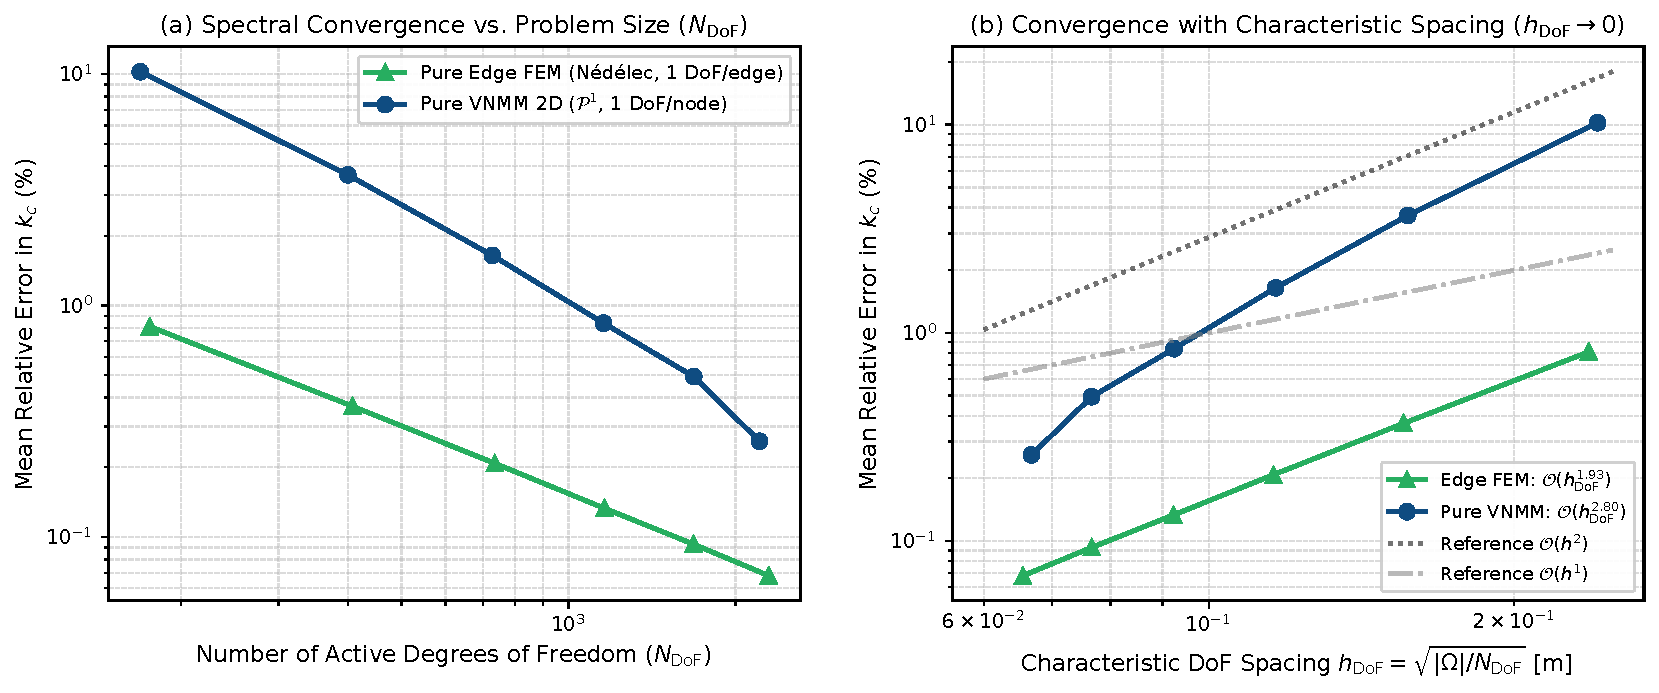
\includegraphics[width=0.98\textwidth]{figura_convergencia_vnmm_vs_fem.pdf}
\caption{Comparative convergence study across 6 refinement levels ($N \in \{9$, $13$, $17$, $21$, $25$, $29\}$): (a) Mean relative spectral error in cutoff wavenumber $k_c$ (\%) as a function of total active degrees of freedom $N_{\mathrm{DoF}}$; (b) Convergence rate as a function of characteristic DoF spacing $h_{\mathrm{DoF}} = \sqrt{|\Omega|/N_{\mathrm{DoF}}}$. Pure Edge FEM exhibits an observed slope of $\mathcal{O}(h_{\mathrm{DoF}}^{1.93})$, while Pure VNMM exhibits an observed fitted slope of $\mathcal{O}(h_{\mathrm{DoF}}^{2.80})$ over the tested refinement interval, demonstrating rapid error reduction without mesh connectivity.}
\label{fig:convergence_vnmm_fem}
\end{figure*}

\subsubsection{Convergence and Efficiency Analysis}
Table~\ref{tab:convergence_6_meshes} and Fig.~\ref{fig:convergence_vnmm_fem} report the convergence history across 6 successive mesh levels ($N \in \{9$, $13$, $17$, $21$, $25$, $29\}$).

\begin{table}[!htbp]
\centering
\caption{Comparative convergence of resonant wavenumber $k_c$ for $TE_z$ modes in a 2D PEC cavity over 6 mesh refinement levels between Edge FEM (Whitney 1st-kind) and Pure VNMM 2D ($\mathcal{P}^1$ complete basis).}
\label{tab:convergence_6_meshes}
\resizebox{\columnwidth}{!}{%
\begin{tabular}{@{} c *{3}{c} *{3}{c} @{}}
\toprule
\textbf{Mesh} & \multicolumn{3}{c}{\textbf{Edge FEM (N\'ed\'elec 1st-kind)}} & \multicolumn{3}{c}{\textbf{Pure VNMM 2D ($\mathcal{P}^1$ Complete Basis)}} \\
\cmidrule(lr){2-4} \cmidrule(lr){5-7}
$N$ & $N_{\mathrm{DoF}}$ & $h_{\mathrm{DoF}}$ [m] & Error (\%) & $N_{\mathrm{DoF}}$ & $h_{\mathrm{DoF}}$ [m] & Error (\%) \\
\midrule
9  & 176  & 0.2368 & 0.810 & 169  & 0.2417 & 10.233 \\
13 & 408  & 0.1555 & 0.367 & 400  & 0.1571 & 3.667 \\
17 & 736  & 0.1158 & 0.208 & 729  & 0.1164 & 1.645 \\
21 & 1160 & 0.0922 & 0.133 & 1156 & 0.0924 & 0.839 \\
25 & 1680 & 0.0766 & 0.093 & 1681 & 0.0766 & 0.493 \\
29 & 2296 & 0.0656 & 0.068 & 2209 & 0.0668 & 0.259 \\
\bottomrule
\end{tabular}%
}
\end{table}

Inspection of the benchmark results reveals several noteworthy numerical properties:
\begin{itemize}
    \item \textbf{Strict Monotonicity:} With the elimination of the artificial determinant tolerance floor ($\mathrm{Tol}_{\mathrm{floor}}$, Eq.~\eqref{eq:scale_dependent_determinant_floor}) on regular grids, the local collocation determinant scales naturally as $\det(\mathbf{A}) \sim \mathcal{O}(h^4)$, allowing nearest-neighbor stencils to be preserved without unphysical support dilation. Consequently, both formulations converge strictly monotonically.
    \item \textbf{Theoretical Error Hierarchy and Absolute Precision:} Throughout all six refinement levels, Edge FEM delivers lower absolute errors (ranging from $0.810\%$ down to $0.068\%$, compared to $10.233\%$ down to $0.259\%$ for VNMM). This baseline accuracy advantage stems from exact closed-contour circulation cancellation via Stokes' theorem along conforming element boundaries in edge elements \cite{nedelec1980mixed, monk2003finite}.
    \item \textbf{Observed Convergence Rates and Pre-Asymptotic Behavior:} While Edge FEM consistently exhibits the canonical second-order rate across all levels ($\mathcal{O}(h_{\mathrm{DoF}}^{1.93})$, with local consecutive slopes tightly bounded between $1.88$ and $2.02$), the Pure VNMM solver displays an observed fitted slope of $\mathcal{O}(h_{\mathrm{DoF}}^{2.80})$ over the six tested refinement levels, with an empirical slope of $\mathcal{O}(h_{\mathrm{DoF}}^{3.24})$ when restricted to the four finest meshes (consecutive two-level slopes progressing from $2.38$ on $N=9 \to 13$, to $2.67$, $2.92$, and $2.84$). 

    Crucially, these steep slopes must be interpreted with caution and should \emph{not} be construed as the theoretical asymptotic convergence order of the method. For a first-order affine polynomial representation $\mathcal{P}^1 \times \mathcal{P}^1$, standard Galerkin variational theory bounds the asymptotic eigenvalue error by $\mathcal{O}(h^2)$ \cite{monk2003finite, boffi1999computational}. The steeper empirical rate observed here reflects coupled pre-asymptotic and variational effects: (i) on coarse meshes, the div-curl penalty introduces an $\mathcal{O}(h)$ divergence error that acts as an artificial numerical stiffness, elevating coarse-grid errors ($10.23\%$ at $N=9$); as $h \to 0$, pointwise divergence error vanishes ($\nabla \cdot \vec{E}^h \to 0$) and this penalty stiffening rapidly dissipates, producing an apparent steepening of the convergence curve; (ii) the six tested resolutions ($N = 9\text{--}29$, $h_{\mathrm{DoF}} \in [0.24, 0.07]$\,m) capture a pre-asymptotic regime where overlapping support stencils dynamically settle; and (iii) the operational metric $h_{\mathrm{DoF}} = \sqrt{|\Omega|/N_{\mathrm{DoF}}}$ serves as a degree-of-freedom scaling proxy rather than a formal element diameter. Therefore, the values $\mathcal{O}(h_{\mathrm{DoF}}^{2.80})$ and $\mathcal{O}(h_{\mathrm{DoF}}^{3.24})$ represent empirical fitted slopes over the tested refinement interval rather than asymptotic convergence orders, illustrating how the meshless formulation overcomes coarse-grid penalty stiffening and closes the accuracy gap with Edge FEM as $h \to 0$.
    \item \textbf{Mesh-Free Discretization Advantage:} While Edge FEM maintains superior absolute accuracy for an identical DoF count on the evaluated regular geometry, the VNMM operates entirely without triangular mesh generation. This eliminates mesh quality degradation, element inversion, and remeshing bottlenecks in geometrically complex or topologically evolving electromagnetic domains.
\end{itemize}

It is important to emphasize the methodological synergy between the support selection strategies: while the absolute tolerance floor ($\mathrm{Tol}_{\mathrm{floor}} = 1.5 \times 10^{-5}$) is indispensable to protect stencils against pathological degeneracies in stochastically perturbed or unconstrained point clouds (Section~\ref{subsec:stochastic_perturbations}), smooth asymptotic refinement on regular grids benefits from allowing the determinant to scale naturally as $\mathcal{O}(h^4)$ to maintain compact nearest-neighbor supports. Combined with the div-curl penalty regularization ($s_{\mathrm{div}} = 6.0$) established in Section~\ref{subsec:cavity_eigenvalues}, the global stiffness matrix $\mathbf{K}$ remains strictly well-conditioned and free of spurious spectral modes within the operational bandwidth across both structured and unstructured discretization regimes.

% ---------------------------------------------------------
% SUBSECTION 6.6: LIMITATIONS AND SCOPE OF APPLICABILITY
% ---------------------------------------------------------
\subsection{Limitations and Scope of Applicability}
\label{subsec:limitations_scope}

While the numerical experiments in Sections~\ref{subsec:conforming_dual_equivalence}--\ref{subsec:convergence_comparison} demonstrate the convergence, conditioning stability, and spectral purity of the proposed VNMM 2D formulation, a mature computational framework requires an explicit delineation of its operational scope, potential failure modes, and methodological limitations \cite{slak2018refined}. We identify seven primary boundaries of applicability:

\begin{enumerate}
    \item \textbf{Background Quadrature Integration Dependency:} 
    Although the local vector shape function construction is completely free of topological mesh connectivity, evaluating the global Ritz-Galerkin weak form (Section~\ref{sec:variational_formulation}) relies on background quadrilateral integration cells with Gauss-Legendre quadrature (EFG-style \cite{belytschko1994element, dolbow1999numerical}). Because the meshless basis functions change supports dynamically across cell boundaries, standard Gauss-Legendre quadrature requires an adequate integration density to capture the non-polynomial weak form terms accurately \cite{dolbow1999numerical}. While the baseline benchmark operates economically with $2 \times 2$ Gauss points per cell ($N_g / N_{\mathrm{DoF}} \approx 1.11$, Section~\ref{subsubsec:quadrature_sensitivity}), our parametric operator analysis demonstrates that full operator convergence ($\|\mathbf{K} - \mathbf{K}_{\mathrm{ref}}\|_F / \|\mathbf{K}_{\mathrm{ref}}\|_F < 8\%$) requires cell refinement and higher-order rules ($4 \times 4$), which unmasks the true spatial discretization floor ($3.32\%$) previously masked by coarse under-integration softening. For domains with highly complex, moving, or multi-scale boundaries, generating conforming background quadrature cells reintroduces a geometric pre-processing burden. Developing truly cell-free integration schemes---such as stabilized conforming nodal integration (SCNI) or meshless local Petrov-Galerkin (MLPG) subdomains \cite{atluri2002meshless}---remains an essential objective for fully unconstrained meshless vector solvers.

    \item \textbf{Local $H(\mathrm{curl})$ Regularity versus Global Non-Conformity:} 
    While each local vector shape function $\vec{N}_i(\mathbf{x})$ is smooth and belongs to $H(\mathrm{curl})$ within its local support domain, the assembled global discrete space is non-conforming on arbitrary point clouds ($V_h \not\subset H(\mathrm{curl}; \Omega)$). Unlike conforming Whitney edge elements, where shared edge circulations enforce exact tangential trace continuity across element facets ($\hat{n} \times [\vec{E}^h] = \mathbf{0}$), the meshless VNMM on unstructured clouds satisfies tangential continuity across dynamically changing support boundaries only in an approximate, weak sense. Consequently, the discrete de Rham complex property $\operatorname{Im}(\nabla) \subset \ker(\nabla \times)$ does not hold exactly at the discrete level, leading to gradient nullspace leakage that requires variational div-curl regularization to prevent low-frequency spectral contamination.

    \item \textbf{Pathological Stencils, Severe Anisotropy, and Support Starvation:} 
    The automated support qualification algorithm (Section~\ref{sec:support_selection_algorithm}) assumes that the candidate search neighborhood contains adequate angular and spatial diversity. Local collocation matrix degeneracies in $\mathbf{A}_{6 \times 6}$ manifest primarily through three geometric failure modes: (i) near-parallel directors ($\ge 4$ directors with mutual angles $< 5^\circ$), which eliminate linear independence among directional projection rows; (ii) near-collinear node distributions ($\ge 5$ nodes aligned along a line, or extreme boundary-layer aspect ratios $\Delta x / \Delta y \gg 10$), which collapse the 2D polynomial Vandermonde submatrix; and (iii) boundary and convex corner starvation, where domain truncation restricts the accessible angular half-space. Although the adaptive $k$-d tree candidate search pool ($K \in [8, 16]$) successfully recovers regular stencils in unconstrained clouds, severe directional clustering necessitates wider neighborhood sampling, resulting in localized support dilation and elevated condition numbers $\kappa_2(\mathbf{A})$.

    \item \textbf{Scale Dependence and Empirical Calibration of Determinant Floor ($\mathrm{Tol}_{\mathrm{floor}}$):} 
    As proven in Section~\ref{subsec:scale_dependent_floor}, the collocation placement determinant scales with the fourth power of spatial dimension, $[\det(\mathbf{A}_{6 \times 6})] = [L]^4$ (Eq.~\eqref{eq:det_quartic_scaling}). Consequently, the absolute tolerance floor $\mathrm{Tol}_{\mathrm{floor}} = 1.5 \times 10^{-5}$ established in this work is calibrated specifically for computational domains with characteristic dimensions on the order of unity ($L_{\mathrm{domain}} \sim \pi$). While the dimensional relation suggests scaling as $\mathrm{Tol}_{\mathrm{floor}} \propto L_{\mathrm{domain}}^4$ or adopting the dimensionless ratio $\tau_{\mathrm{rel}} = |\det(\mathbf{A})| / h_{\mathrm{local}}^4$, it has not yet been demonstrated that this simple scaling rule produces a parameter directly transferable across arbitrary geometries, non-uniform nodal density gradients, or severe directional anisotropies. Hence, the threshold should be viewed as an effective empirical parameter calibrated for the tested benchmark configurations rather than a universal invariant.

    \item \textbf{Div-Curl Penalty Sensitivity and Numerical Over-Stiffening:} 
    The Ritz-Galerkin div-curl regularization shifts non-physical gradient nullspace modes to the high-frequency spectrum for penalty values $s_{\mathrm{div}} \in [4.0, 10.0]$ with minimal perturbation to physical resonant frequencies ($R_{\mathrm{div}} \le 1\%$). However, because discrete divergence at Gauss quadrature points is only weakly enforced ($\nabla \cdot \vec{E}^h \sim \mathcal{O}(h)$), setting an excessively large penalty parameter ($s_{\mathrm{div}} \gg 50$) exerts an artificial volumetric over-stiffening (locking) effect on solenoidal fields, deteriorating field convergence rates and inflating global matrix condition numbers. Conversely, taking $s_{\mathrm{div}} \to 0$ allows spurious gradient modes to re-enter the physical operational bandwidth.

    \item \textbf{High-Frequency Electromagnetics and Numerical Dispersion:} 
    The eigenvalue benchmarks presented in Section~\ref{subsec:cavity_eigenvalues} validate the spectral behavior across the lower cavity resonant modes ($\lambda \le 20$). In high-frequency, short-wavelength regimes ($kh \gg 1$), all discrete wave solvers suffer from numerical dispersion and phase lag (the pollution effect) \cite{jin2014finite, monk2003finite}. For the VNMM, maintaining phase accuracy requires satisfying the standard spatial sampling criterion ($h \le \lambda_{\mathrm{EM}} / 10$). Furthermore, for electrically large domains, the penalty parameter $s_{\mathrm{div}}$ may require frequency-dependent scaling to ensure consistent spectral separation between physical and non-physical modes.

    \item \textbf{Dimensional Scope (2D Formulation) and Non-Linear Media:} 
    The mathematical formulation and numerical experiments in this work are developed for two-dimensional electromagnetic vector fields ($xy$-plane, $TE_z$ polarization). Extending the complete vector basis to three dimensions requires a 12-dimensional polynomial space $\mathcal{P}_1 \times \mathcal{P}_1 \times \mathcal{P}_1$ ($M_{\mathrm{supp}} = 12$ support nodes per stencil) \cite{goncalves2023vector}, which substantially expands the combinatorial candidate pool $\binom{K}{12}$ and introduces 3D surface-integral boundary representations. Additionally, extending the regularized VNMM framework to non-linear eddy-current problems with ferromagnetic saturation ($B\text{--}H$ curves) necessitates iterative Newton-Raphson linearizations and time-stepping schemes \cite{tsukerman1992overlapping, coppoli2012induction}.
\end{enumerate}

% =========================================================
% SECTION 6: CONCLUSION AND FUTURE WORKS
% =========================================================
\section{Conclusion and Future Works}
\label{sec:conclusion}

This paper has presented an investigation into the mathematical, algebraic, and variational aspects of the Vector Nodal Meshless Method (VNMM 2D) applied to electromagnetic vector field interpolation and resonant cavity eigenvalue analysis. By identifying the origin of curl stagnation in early solenoidal vector meshless formulations and addressing stencil ill-conditioning, this work establishes a stabilized framework for vector approximation on unstructured point clouds without mesh connectivity.

\subsection{Summary of Core Contributions and Key Findings}
\label{subsec:summary_contributions}

A central objective of this work was to overcome the topological mesh dependence present in early VNMM studies \cite{ortiz2023tese, goncalves2025tese}. In foundational formulations, candidate support selection relied on background geometric scaffolding, such as planar subdivisions or Delaunay triangulations, to prevent algebraic placement degeneracies. The present work addresses this dependency, demonstrating that the VNMM can be formulated directly on \textbf{unstructured node distributions and arbitrary vector director orientations} within the tested configurations without requiring auxiliary planar subdivisions or background mesh connectivity for local shape function construction.

The primary methodological contributions and validation findings of this research are summarized as follows:

\textbf{Primary Methodological Contributions:}
\begin{enumerate}
    \item \textbf{Exact Local Dual Equivalence to Whitney Edge Elements:} 
    We proved and verified numerically down to machine precision ($\approx 10^{-16}$) that on conforming simplicial elements, the 3-node VNMM $\mathcal{L}^1$ is constructively isomorphic to canonical Whitney 1-form edge elements. This establishes that the $\mathcal{O}(1)$ curl stagnation observed in earlier meshless implementations is not an intrinsic defect of the solenoidal space $\mathcal{L}^1$ itself, but rather arises from deploying an incomplete polynomial basis within a pointwise collocation framework devoid of closed-contour line integrals.

    \item \textbf{Resolution of Modal Aliasing via Complete $\mathcal{P}^1$ Vector Basis:} 
    Transitioning from the incomplete solenoidal space $\mathcal{L}^1$ to the complete affine polynomial vector space $\mathcal{P}^1 = \mathcal{P}_1 \times \mathcal{P}_1$ ($M_{\mathrm{supp}} = 6$ nodes) restores the full 4-component local Jacobian representation $\{\partial E_x/\partial x$, $\partial E_x/\partial y$, $\partial E_y/\partial x$, $\partial E_y/\partial y\}$. In the tested point-cloud collocation setting, this eliminates the derivative aliasing mechanism of $\mathcal{L}^1$, overcoming the observed $\mathcal{O}(1)$ curl stagnation plateau and achieving first-order curl convergence ($\mathcal{O}(h^{0.97})$) alongside an observed empirical superconvergence of $\mathcal{O}(h^{2.17})$ for electric field interpolation on the evaluated analytical $TE_{11}$ cavity benchmark.

    \item \textbf{Automated Support Selection and Algebraic Stabilization on Irregular Clouds:} 
    By replacing pre-defined geometric subdivisions with an automated selection algorithm coupling $k$-d tree spatial queries with scale-dependent determinant thresholding ($[\det(\mathbf{A}_{6\times6})] = [L]^4$), the approach identifies admissible, well-conditioned support sextets across irregular node distributions. Incorporating an absolute tolerance floor ($\operatorname{Tol}_{\mathrm{floor}} = 1.5 \times 10^{-5}$) filters out near-singular stencils in the tested configurations, bounding condition numbers ($\kappa_2(\mathbf{A}) \le 73$ at the baseline floor, decreasing to $\approx 64$ at the compromise threshold $3.0 \times 10^{-5}$) and preserving monotonic convergence under $25\%$ stochastic spatial jitter and random director orientations in the evaluated realization.
\end{enumerate}

\textbf{Spectral Validation and Benchmark Findings:}
\begin{enumerate}
    \item \textbf{Spectral Behavior in Resonant Cavity Benchmarks:} 
    In the tested transverse electric ($TE_z$) resonant cavity setup, discrete gradient nullspace leakage ($\nabla \times (\nabla \phi) \neq \mathbf{0}$ at quadrature points) is controlled through a Ritz-Galerkin weak formulation with div-curl penalty regularization. Selecting $s_{\mathrm{div}} = 6.0$ as a representative value within the stable penalty range shifts non-physical gradient states beyond the tested operational frequency window ($\lambda > 50$), producing clean modal pairing and restricting the mean cutoff wavenumber error to approximately $1.00\%$ on the baseline benchmark grid.

    \item \textbf{Convergence Trend Relative to Canonical Edge FEM:} 
    A comparative benchmark across six refinement levels confirmed that the stabilized VNMM displays an observed empirical fitted slope of $\mathcal{O}(h_{\mathrm{DoF}}^{2.80})$ over the tested refinement interval (compared to $\mathcal{O}(h_{\mathrm{DoF}}^{1.93})$ for Whitney 1-form edge elements). While Edge FEM retains superior absolute precision per degree of freedom on regular geometries, the meshless formulation progressively reduces the coarse-grid gap as $h \to 0$ while operating without conforming mesh connectivity.
\end{enumerate}

\subsection{Promising Directions for Future Research}
\label{subsec:future_works}

Building upon the 2D vector meshless formulation developed and validated in this work, several important open questions and extensions remain for future research:

\begin{enumerate}
    \item \textbf{Extension to 3D Vector Nodal Meshless Formulations (3D VNMM):} 
    Extending the complete polynomial space concept to three-dimensional vector domains ($\mathcal{P}^1$ in 3D, requiring $M_{\mathrm{supp}} = 12$ support nodes) to solve complex 3D high-frequency waveguiding and radiation problems \cite{goncalves2023vector}.

    \item \textbf{Conforming Hybrid FEM-VNMM Domain Decomposition:} 
    Establishing direct master-slave hybrid coupling between boundary-conforming Whitney edge finite elements and interior VNMM unconstrained point clouds through exact dimensional scale mapping, combining boundary geometric fidelity with mesh-free volume discretization.

    \item \textbf{Non-Linear Electromagnetic Applications and Motion Modeling:} Extending the regularized VNMM 2D solvers to transient non-linear eddy-current problems, incorporating $B\text{--}H$ iron core saturation, field-circuit coupling, and electrical machine rotor movement modeling without remeshing \cite{tsukerman1992overlapping, coppoli2012induction}.

    \item \textbf{Adaptive Meshless Refinement ($h$- and $p$-Adaptivity):} 
    Developing a posteriori local residual error estimators based on the placement determinant $|\det(\mathbf{A})|$ and local curl jump indicators to drive automatic node insertion ($h$-adaptivity) and local polynomial order elevation ($p$-adaptivity) around re-entrant corners and material interfaces.

    \item \textbf{High-Performance Parallel Computing and GPU Acceleration:} 
    Accelerating the point-based Element-Free Galerkin (EFG) Gauss integration loop and local placement matrix inversions through massively parallel CUDA/GPU implementations, exploiting the decoupled nature of local $k$-d tree candidate queries.
\end{enumerate}


\section*{Declaration of Generative AI and AI-Assisted Technologies in the Writing Process}
During the preparation of this work, the authors used Google Antigravity / Gemini in order to assist with English language editing, LaTeX code formatting, script automation for numerical data consistency, and cross-referencing verification. After using this tool, the authors carefully reviewed, verified, and edited all resulting content and take full responsibility for the integrity and accuracy of the publication.


% --- AGRADECIMENTOS ---
\section*{Acknowledgements}
The authors would like to thank the Brazilian research funding agencies CAPES, CNPq, and FAPEMIG for their financial support during the development of this research project.

% --- REFERÊNCIAS BIBLIOGRÁFICAS ---
\bibliographystyle{elsarticle-num}
\bibliography{references}

\end{document}

\endinput
%%
%% End of file `elsarticle-template-num.tex'.